% ============================================================
% The Building Blocks of LLMs: A Mathematical History
% From Archimedes to Attention: 2,000+ Years of Mathematics Inside Your AI
% Target Audience: High School Seniors (Mathematics)
% Duration: ~93 minutes (3 sessions recommended)
% Companion lecture to "The Story of Mathematics: 5,000 Years of Human Genius"
% ============================================================
\documentclass[aspectratio=169,12pt]{beamer}

% ---- Theme & Colors ----
\usetheme{Madrid}
\usecolortheme{whale}

% Custom color palette (shared with main lecture)
\definecolor{babylonBrown}{RGB}{139,90,43}
\definecolor{greekBlue}{RGB}{0,71,171}
\definecolor{indianSaffron}{RGB}{204,119,34}
\definecolor{chineseRed}{RGB}{170,56,30}
\definecolor{islamicGreen}{RGB}{0,128,55}
\definecolor{medievalPurple}{RGB}{102,51,153}
\definecolor{renaissanceGold}{RGB}{184,134,11}
\definecolor{enlightenmentTeal}{RGB}{0,128,128}
\definecolor{modernSteel}{RGB}{70,130,180}
\definecolor{digitalBlue}{RGB}{30,80,162}
\definecolor{aiViolet}{RGB}{106,13,173}
\definecolor{accentOrange}{RGB}{230,126,34}
\definecolor{darkBg}{RGB}{30,30,30}

% LLM-specific section colors
\definecolor{linalgTeal}{RGB}{0,150,136}
\definecolor{calculusRed}{RGB}{211,47,47}
\definecolor{probBlue}{RGB}{25,118,210}
\definecolor{infoAmber}{RGB}{255,160,0}
\definecolor{logicGray}{RGB}{97,97,97}
\definecolor{approxGreen}{RGB}{56,142,60}
\definecolor{neuronPink}{RGB}{194,24,91}
\definecolor{seqIndigo}{RGB}{63,81,181}

% Set main beamer colors - aiViolet as primary for this lecture
\setbeamercolor{palette primary}{bg=aiViolet,fg=white}
\setbeamercolor{palette secondary}{bg=aiViolet!80,fg=white}
\setbeamercolor{palette tertiary}{bg=aiViolet!60,fg=white}
\setbeamercolor{frametitle}{bg=aiViolet,fg=white}
\setbeamercolor{title}{bg=aiViolet,fg=white}
\setbeamercolor{section in toc}{fg=aiViolet}
\setbeamercolor{block title}{bg=aiViolet,fg=white}
\setbeamercolor{block body}{bg=aiViolet!5}
\setbeamercolor{item}{fg=aiViolet}

% ---- Fonts ----
\usefonttheme{professionalfonts}
\setbeamerfont{title}{size=\Large,series=\bfseries}
\setbeamerfont{frametitle}{size=\large,series=\bfseries}
\setbeamerfont{framesubtitle}{size=\normalsize,series=\mdseries}

% ---- Packages ----
\usepackage[utf8]{inputenc}
\usepackage[T1]{fontenc}
\usepackage{amsmath,amssymb,amsfonts}
\usepackage{graphicx}
\usepackage{tikz}
\usetikzlibrary{shapes,arrows.meta,positioning,calc,decorations.pathmorphing,backgrounds,fit}
\usepackage{booktabs}
\usepackage{multicol}
\usepackage{hyperref}
\usepackage{fontawesome5}
\usepackage{xcolor}
\usepackage{pgfplots}
\pgfplotsset{compat=1.18}
\usepackage{tcolorbox}
\tcbuselibrary{skins,breakable}

% ---- Custom Commands ----

% Person info box
\newtcolorbox{personbox}[2][]{%
  colback=#2!5,
  colframe=#2,
  fonttitle=\bfseries,
  title=#1,
  rounded corners,
  boxrule=1pt,
  left=4pt,right=4pt,top=4pt,bottom=4pt
}

% Key insight callout
\newtcolorbox{insightbox}{%
  colback=accentOrange!10,
  colframe=accentOrange,
  fonttitle=\bfseries,
  title={\faLightbulb\ Key Insight},
  rounded corners,
  boxrule=1pt,
  left=4pt,right=4pt,top=4pt,bottom=4pt
}

% Connection to LLM callout
\newtcolorbox{llmconnection}{%
  colback=aiViolet!8,
  colframe=aiViolet,
  fonttitle=\bfseries,
  title={\faRobot\ Inside the LLM},
  rounded corners,
  boxrule=1pt,
  left=4pt,right=4pt,top=4pt,bottom=4pt
}

% Visual placeholder
\newcommand{\visualplaceholder}[2][6cm]{%
  \begin{center}
  \fbox{\parbox[c][3cm]{\dimexpr#1-1cm\relax}{\centering\small\itshape\color{gray}\faImage\ #2}}
  \end{center}
}

% Verify tag (for speaker notes)
\newcommand{\verifytag}[1]{\textcolor{red!70}{\textbf{[VERIFY:} \textit{#1}\textbf{]}}}

% Session break slide
\newcommand{\sessionbreak}[2]{%
  \begin{frame}[plain]
    \begin{tikzpicture}[remember picture,overlay]
      \fill[aiViolet] (current page.south west) rectangle (current page.north east);
      \node[text=white,font=\Huge\bfseries] at (current page.center) {#1};
      \node[text=white!80,font=\large,below=1cm of current page.center] {#2};
    \end{tikzpicture}
  \end{frame}
}

% Slide counter in footline
\setbeamertemplate{footline}{%
  \leavevmode%
  \hbox{%
    \begin{beamercolorbox}[wd=.333333\paperwidth,ht=2.25ex,dp=1ex,center]{author in head/foot}%
      \usebeamerfont{author in head/foot}\insertshortauthor
    \end{beamercolorbox}%
    \begin{beamercolorbox}[wd=.333333\paperwidth,ht=2.25ex,dp=1ex,center]{title in head/foot}%
      \usebeamerfont{title in head/foot}\insertshorttitle
    \end{beamercolorbox}%
    \begin{beamercolorbox}[wd=.333333\paperwidth,ht=2.25ex,dp=1ex,right]{date in head/foot}%
      \usebeamerfont{date in head/foot}\insertframenumber{} / \inserttotalframenumber\hspace*{2ex}
    \end{beamercolorbox}}%
  \vskip0pt%
}

% Remove navigation symbols
\setbeamertemplate{navigation symbols}{}

% ---- Document Info ----
\title[Building Blocks of LLMs]{The Building Blocks of LLMs\\[0.3em]{\large From Archimedes to Attention}}
\subtitle{2,000+ Years of Mathematics Inside Your AI}
\author{Prof.\ J.\ Osterrieder}
\date{2026}
\institute{}

% ============================================================
\begin{document}

% ---- Part 1: Opening + Linear Algebra + Calculus & Optimization ----
% ============================================================
% Building Blocks of LLMs -- Part 1
% Section 0: Opening (Slides 1-4)
% Section 1: Linear Algebra (Slides 5-16)
% Section 2: Calculus & Optimization (Slides 17-25)
% ============================================================

% ============================================================
% SECTION 0: OPENING (Slides 1-4)
% ============================================================
\section{Opening}

% ----------------------------------------------------------
% Slide 1: Title Slide
% ----------------------------------------------------------
\begin{frame}[plain]
  \begin{tikzpicture}[remember picture, overlay]
    \fill[aiViolet] (current page.south west) rectangle (current page.north east);
  \end{tikzpicture}

  \vspace{1cm}
  \begin{center}
    {\Huge\bfseries\textcolor{white}{The Building Blocks of LLMs}}\\[0.6em]
    {\Large\textcolor{white!90}{A Mathematical History}}\\[1.5em]
    {\large\textcolor{white!80}{From Archimedes to Attention:}}\\[0.3em]
    {\large\textcolor{white!80}{2,000+ Years of Mathematics Inside Your AI}}\\[2em]
    {\normalsize\textcolor{white!70}{Prof.\ J.\ Osterrieder \hspace{2em} 2026}}
  \end{center}

  \note{
    Welcome slide. Frame the lecture: this is not about hype or ``intelligence.''
    This is about tracing every mathematical component of the LLMs students use daily
    back to the person who invented it.
    Core throughline: ``Every component of an LLM was invented by someone,
    for a specific purpose, often centuries before AI existed.''
    Audience takeaway: ``I already know some of this math ---
    I just didn't know it was inside my AI.''
  }
\end{frame}

% ----------------------------------------------------------
% Slide 2: What's Inside Your AI?
% ----------------------------------------------------------
\begin{frame}{What's Inside Your AI?}

  \begin{columns}[T]
    \begin{column}{0.45\textwidth}
      \vspace{0.5em}
      When you type a question to ChatGPT or Claude\ldots

      \vspace{0.5em}
      The machine that answers is built \alert{entirely from mathematics}.

      \vspace{0.5em}
      \begin{itemize}
        \item Not magic
        \item Not ``intelligence''
        \item \textbf{Specific math}, invented by \textbf{specific people},\\
              at \textbf{specific times}
      \end{itemize}

      \vspace{0.8em}
      \begin{insightbox}
        You already know some of this math.
        You just don't know it's inside your AI yet.
      \end{insightbox}
    \end{column}

    \begin{column}{0.52\textwidth}
      % -- Slide 2: Smartphone with math-topic arrows --
      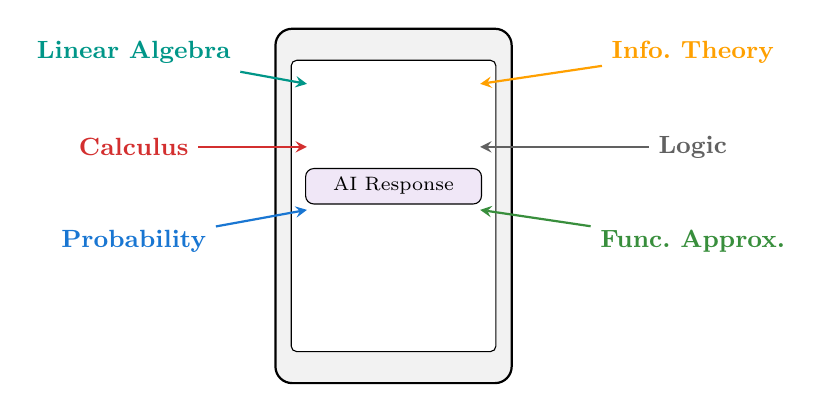
\begin{tikzpicture}[
        every node/.style={font=\small\bfseries},
        arr/.style={->,>=stealth,thick}
      ]
        % Smartphone outline
        \draw[rounded corners=6pt, thick, fill=gray!10]
          (0,0) rectangle (3,4.5);
        \draw[rounded corners=2pt, fill=white]
          (0.2,0.4) rectangle (2.8,4.1);
        % Chat bubble inside
        \node[draw, rounded corners=3pt, fill=aiViolet!10,
              text width=2cm, align=center, font=\scriptsize]
          (chat) at (1.5,2.5) {AI Response};
        % Six labeled arrows from outside pointing in
        \node[text=linalgTeal] (la) at (-1.8,4.2) {Linear Algebra};
        \draw[arr, linalgTeal] (la) -- (0.4,3.8);
        \node[text=calculusRed] (ca) at (-1.8,3.0) {Calculus};
        \draw[arr, calculusRed] (ca) -- (0.4,3.0);
        \node[text=probBlue] (pr) at (-1.8,1.8) {Probability};
        \draw[arr, probBlue] (pr) -- (0.4,2.2);
        \node[text=infoAmber] (it) at (5.3,4.2) {Info.\ Theory};
        \draw[arr, infoAmber] (it) -- (2.6,3.8);
        \node[text=logicGray] (lo) at (5.3,3.0) {Logic};
        \draw[arr, logicGray] (lo) -- (2.6,3.0);
        \node[text=approxGreen] (fa) at (5.3,1.8) {Func.\ Approx.};
        \draw[arr, approxGreen] (fa) -- (2.6,2.2);
      \end{tikzpicture}
    \end{column}
  \end{columns}

  \note{
    Key message: the AI they use every day is made of math they can learn to understand.
    ``You already know some of this math. You just don't know it's inside your AI yet.
    Today we're going to fix that.''
    Do NOT use hype language. Let the math speak for itself.
  }
\end{frame}

% ----------------------------------------------------------
% Slide 3: The Exploded Diagram -- What We Will Build Today
% ----------------------------------------------------------
\begin{frame}{The Exploded Transformer --- What We Will Build Today}

  \begin{center}
    \visualplaceholder[12cm]{EXPLODED TRANSFORMER DIAGRAM (full-slide, to be generated as figures/exploded-transformer-base.pdf).
      Components to show, color-coded by section:
      (1) Embedding layer -- lookup table, word $\to$ vector [linalgTeal]
      (2) Positional encoding -- sinusoidal waves added to embeddings [seqIndigo]
      (3) Multi-head attention block -- Q/K/V projections, scaled dot-product, concat + linear [linalgTeal + probBlue]
      (4) Add \& Norm (residual connection + layer normalization) [neuronPink]
      (5) Feed-forward network -- two linear layers with activation [approxGreen + neuronPink]
      (6) Second Add \& Norm [neuronPink]
      (7) Repeat $\times N$ layers indicator [logicGray]
      (8) Output linear projection + softmax [probBlue + infoAmber]
      (9) Loss computation -- cross-entropy [infoAmber + calculusRed]
      (10) Backpropagation arrows flowing backward through all layers [calculusRed]
      Layout: vertical stack (input at bottom, output at top), each component a labeled rounded box.
      Intentionally overwhelming on first view.}
  \end{center}

  \vspace{-0.3em}
  {\small\centering\textcolor{gray}{This looks complicated now. By the end, you will know every piece --- and WHO invented it.}\par}

  \note{
    ``This looks complicated right now. Good. By the end of today, you'll know what
    every one of these pieces does and WHO invented it.''
    This slide is meant to overwhelm --- we will return to it in Slide 73
    with full understanding.
    Each color maps to a section of the lecture.
    Do not explain the components yet; just let students absorb the visual.
  }
\end{frame}

% ----------------------------------------------------------
% Slide 4: The Convergence Diagram -- Our Roadmap
% ----------------------------------------------------------
\begin{frame}{Our Roadmap --- The Convergence Diagram}

  \begin{center}
    \visualplaceholder[12cm]{CONVERGENCE DIAGRAM -- INITIAL STATE (to be generated as figures/convergence-0.pdf).
      Layout: central large circle with ``?'' in gray.
      10 satellite nodes in a semicircle (180\textdegree{} arc, evenly spaced), all in gray:
      (1) Linear Algebra [1809--1900s]
      (2) Calculus \& Optimization [c.\,250\,BCE--1986]
      (3) Probability \& Statistics [1654--1933]
      (4) Information Theory [1865--1948]
      (5) Logic \& Computation [1854--1970s]
      (6) Function Approximation [1807--1991]
      (7) The Neuron \& Depth [1943--2016]
      (8) Sequence Modeling [1906--2014]
      (9) The Transformer [2017]
      (10) Scaling to LLMs [2018--2026]
      Gray dashed arrows from each satellite toward center.
      All nodes dim/unlit. Target colors when lit: linalgTeal, calculusRed, probBlue, infoAmber, logicGray, approxGreen, neuronPink, seqIndigo, aiViolet, accentOrange.}
  \end{center}

  \note{
    ``We're going to light up these nodes one by one. Each one is a piece of math
    that somebody invented, often for a completely different purpose, that ended up
    inside the machines you use every day.''
    This diagram will recur at the end of every section, progressively lighting up.
    Emphasize: ten branches of mathematics, developed over 2,000+ years,
    all converge in one architecture.
  }
\end{frame}


% ============================================================
% SECTION 1: LINEAR ALGEBRA -- "The Skeleton of Neural Networks"
% Slides 5-16
% ============================================================
\section{Linear Algebra}

% ----------------------------------------------------------
% Slide 5: Section Divider
% ----------------------------------------------------------
{
\setbeamercolor{background canvas}{bg=digitalBlue}
\begin{frame}[plain]
  \centering
  \vspace{1.5cm}
  \textcolor{white}{\Huge\bfseries Linear Algebra}\\[0.6em]
  \textcolor{white!80}{\large The Skeleton of Neural Networks}\\[1em]
  \textcolor{white!60}{\normalsize 1809--1900s}\\[1.5em]
  \textcolor{white!70}{\itshape``Neural networks are, at their core, matrix multiplication machines.''}

  \note{
    Section transition. Linear algebra provides the fundamental data structures
    (vectors, matrices) and operations (multiplication, dot product) of neural networks.
    Timeline: formal theory begins around 1809 (Grassmann born), but roots in Gauss and earlier.
    Convergence diagram: Section 1 node pulsing.
  }
\end{frame}
}

% ----------------------------------------------------------
% Slide 6: What Is a Vector?
% ----------------------------------------------------------
\begin{frame}{What Is a Vector? --- Forces, Velocities, and Words}

  \begin{columns}[T]
    \begin{column}{0.52\textwidth}
      \begin{personbox}[Hermann Grassmann (1809--1877)]{digitalBlue}
        \small
        \textbf{Origin:} Stettin, Prussia (now Szczecin, Poland)\\
        \textbf{Key work:} \emph{Die lineale Ausdehnungslehre} (1844) ---
        the first general theory of vector spaces in any number of dimensions.\\
        A schoolteacher whose work was so ahead of its time that almost nobody read it.
      \end{personbox}

      \vspace{0.3em}
      \begin{personbox}[Sir William Rowan Hamilton (1805--1865)]{digitalBlue}
        \small
        \textbf{Origin:} Dublin, Ireland\\
        \textbf{Key work:} Invented quaternions (1843) while walking along the Royal Canal
        in Dublin --- famously carved the formula into Brougham Bridge.
      \end{personbox}
    \end{column}

    \begin{column}{0.45\textwidth}
      A \textbf{vector} is a list of numbers that represents something.

      \vspace{0.5em}
      % -- Slide 6: 2D, 3D, and 768-dim vectors --
      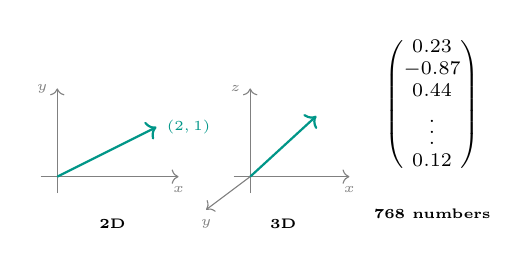
\begin{tikzpicture}[scale=0.7]
        % 2D vector
        \draw[->,gray,thin] (-0.3,0)--(2.2,0) node[below,font=\tiny]{$x$};
        \draw[->,gray,thin] (0,-0.3)--(0,1.6) node[left,font=\tiny]{$y$};
        \draw[->,thick,linalgTeal] (0,0)--(1.8,0.9)
          node[right,font=\tiny]{$(2,1)$};
        \node[below,font=\tiny\bfseries] at (1,-.6) {2D};
        % 3D vector (pseudo-isometric)
        \begin{scope}[xshift=3.5cm]
          \draw[->,gray,thin] (-0.3,0)--(1.8,0) node[below,font=\tiny]{$x$};
          \draw[->,gray,thin] (0,-0.3)--(0,1.6) node[left,font=\tiny]{$z$};
          \draw[->,gray,thin] (0,0)--(-0.8,-0.6) node[below,font=\tiny]{$y$};
          \draw[->,thick,linalgTeal] (0,0)--(1.2,1.1);
          \node[below,font=\tiny\bfseries] at (0.6,-.6) {3D};
        \end{scope}
        % 768-dim column vector
        \begin{scope}[xshift=6.8cm, yshift=0.3cm]
          \node[font=\scriptsize,align=center] at (0,1.0) {$\begin{pmatrix}0.23\\-0.87\\0.44\\\vdots\\0.12\end{pmatrix}$};
          \node[below,font=\tiny\bfseries] at (0,-0.7) {768 numbers};
        \end{scope}
      \end{tikzpicture}

      \vspace{0.1em}
      {\scriptsize In an LLM, each word becomes a vector --- a list of 768+ numbers.}

      \vspace{0.3em}
      % -- Slide 6: Brougham Bridge plaque recreation --
      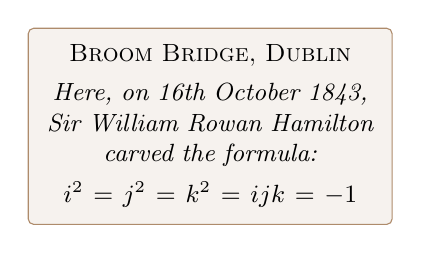
\begin{tikzpicture}
        \node[draw=babylonBrown!70, fill=babylonBrown!8, rounded corners=2pt,
              inner sep=6pt, text width=4.2cm, align=center,
              font=\small] {
          \textsc{Broom Bridge, Dublin}\\[3pt]
          {\itshape Here, on 16th October 1843,}\\
          {\itshape Sir William Rowan Hamilton}\\
          {\itshape carved the formula:}\\[4pt]
          $i^{2} = j^{2} = k^{2} = ijk = -1$
        };
      \end{tikzpicture}
    \end{column}
  \end{columns}

  \note{
    ``Hamilton was so excited that he carved his formula into a bridge. Grassmann's
    far more general idea was ignored for decades. Both were building the language
    that neural networks would eventually speak.''
    LLM connection: every word is converted into a vector (an ``embedding'')
    with 768 or more numbers. Grassmann's abstract vector spaces ARE the embedding
    spaces of modern AI.
    \verifytag{Grassmann's 1844 publication date and characterization of reception.}
  }
\end{frame}

% ----------------------------------------------------------
% Slide 7: Modern Vector Notation -- Gibbs and Heaviside
% ----------------------------------------------------------
\begin{frame}{Modern Vector Notation --- Gibbs and Heaviside}

  \begin{columns}[T]
    \begin{column}{0.50\textwidth}
      \begin{personbox}[Josiah Willard Gibbs (1839--1903)]{digitalBlue}
        \small
        \textbf{Origin:} New Haven, Connecticut, USA\\
        \textbf{Key work:} Extracted the useful vector parts from Hamilton's
        quaternions; created modern vector analysis
        (lecture notes \emph{Elements of Vector Analysis}, c.\,1881--1884).
      \end{personbox}

      \vspace{0.3em}
      \begin{personbox}[Oliver Heaviside (1850--1925)]{digitalBlue}
        \small
        \textbf{Origin:} London, England\\
        \textbf{Key work:} Self-taught electrical engineer who independently developed
        vector calculus; reformulated Maxwell's equations into their compact modern form.
      \end{personbox}
    \end{column}

    \begin{column}{0.47\textwidth}
      % -- Slide 7: Quaternion vs vector notation --
      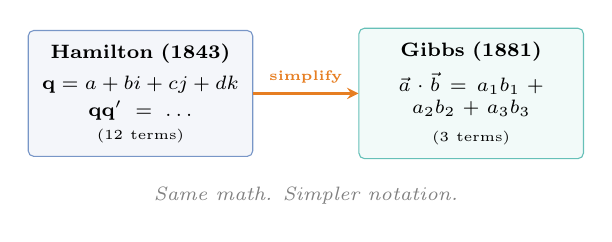
\begin{tikzpicture}
        % Hamilton box
        \node[draw=digitalBlue!60, fill=digitalBlue!5, rounded corners=2pt,
              text width=2.5cm, align=center, inner sep=5pt,
              font=\scriptsize] (ham) at (0,0) {
          \textbf{Hamilton (1843)}\\[3pt]
          $\mathbf{q}= a + bi + cj + dk$\\[2pt]
          $\mathbf{q}\mathbf{q'} = \ldots$\\
          {\tiny (12 terms)}
        };
        % Gibbs box
        \node[draw=linalgTeal!60, fill=linalgTeal!5, rounded corners=2pt,
              text width=2.5cm, align=center, inner sep=5pt,
              font=\scriptsize] (gib) at (4.2,0) {
          \textbf{Gibbs (1881)}\\[3pt]
          $\vec{a} \cdot \vec{b} = a_1 b_1 + a_2 b_2 + a_3 b_3$\\[2pt]
          {\tiny (3 terms)}
        };
        % Arrow between
        \draw[->,>=stealth,thick,accentOrange] (ham) -- (gib)
          node[midway,above,font=\tiny\bfseries] {simplify};
        % Caption
        \node[font=\scriptsize\itshape, text=gray] at (2.1,-1.3)
          {Same math. Simpler notation.};
      \end{tikzpicture}
    \end{column}
  \end{columns}

  \note{
    ``Gibbs and Heaviside were not trying to build AI. They were trying to make
    physics easier to write down. But their notation is exactly what we use to
    describe neural networks today.''
    \verifytag{Gibbs's lecture notes dated 1881--1884. Confirm exact years of the
    two printings.}
  }
\end{frame}

% ----------------------------------------------------------
% Slide 8: Matrices -- Cayley and Sylvester
% ----------------------------------------------------------
\begin{frame}{Matrices --- Cayley and Sylvester}

  \begin{columns}[T]
    \begin{column}{0.50\textwidth}
      \begin{personbox}[Arthur Cayley (1821--1895)]{digitalBlue}
        \small
        \textbf{Origin:} Richmond, Surrey, England\\
        \textbf{Key work:} ``A Memoir on the Theory of Matrices'' (1858) ---
        established matrices as algebraic objects in their own right.\\
        Also a practicing lawyer for 14 years before returning to academia.
      \end{personbox}

      \vspace{0.3em}
      \begin{personbox}[James Joseph Sylvester (1814--1897)]{digitalBlue}
        \small
        \textbf{Origin:} London, England\\
        \textbf{Key work:} Coined the word ``matrix'' (1850), from Latin for
        ``womb'' --- he saw it as something from which determinants are born.
        Also coined ``discriminant,'' ``invariant,'' and many other terms.
      \end{personbox}
    \end{column}

    \begin{column}{0.47\textwidth}
      % -- Slide 8: Small matrix vs huge LLM matrix --
      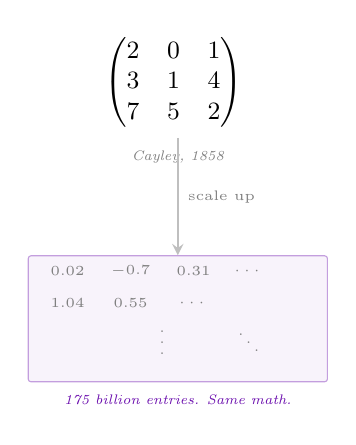
\begin{tikzpicture}
        % Small 3x3 matrix
        \node[font=\small, align=center] (small) at (0,1.5) {
          $\begin{pmatrix}
            2 & 0 & 1\\
            3 & 1 & 4\\
            7 & 5 & 2
          \end{pmatrix}$
        };
        \node[font=\tiny\itshape, text=gray, below=1pt of small] {Cayley, 1858};
        % Large LLM weight matrix suggestion
        \node[draw=aiViolet!40, fill=aiViolet!5, minimum width=3.8cm,
              minimum height=1.6cm, rounded corners=1pt] (big) at (0,-1.5) {};
        \node[font=\tiny, text=gray] at (-1.4,-0.9) {0.02};
        \node[font=\tiny, text=gray] at (-0.6,-0.9) {$-$0.7};
        \node[font=\tiny, text=gray] at (0.2,-0.9) {0.31};
        \node[font=\tiny, text=gray] at (0.9,-0.9) {$\cdots$};
        \node[font=\tiny, text=gray] at (-1.4,-1.3) {1.04};
        \node[font=\tiny, text=gray] at (-0.6,-1.3) {0.55};
        \node[font=\tiny, text=gray] at (0.2,-1.3) {$\cdots$};
        \node[font=\tiny, text=gray] at (-0.2,-1.7) {$\vdots$};
        \node[font=\tiny, text=gray] at (0.9,-1.7) {$\ddots$};
        \node[font=\tiny\itshape, text=aiViolet, below=1pt of big]
          {175 billion entries. Same math.};
        % Arrow
        \draw[->,>=stealth,thick,gray!50] (small) -- (big)
          node[midway,right,font=\tiny,text=gray] {scale up};
      \end{tikzpicture}
    \end{column}
  \end{columns}

  \note{
    ``Sylvester literally named it. `Matrix' --- from Latin for `womb.'
    He thought of it as something that gives birth to numbers.
    He had no idea it would give birth to AI.''
    LLM connection: every layer in a neural network is defined by a matrix of
    ``weights.'' When your prompt passes through GPT, it is multiplied by dozens
    of these matrices. Each one was learned during training.
    \verifytag{Cayley's 1858 paper title. Sylvester's coinage of ``matrix''
    in 1850 --- some sources say 1848. Verify exact year and publication.}
  }
\end{frame}

% ----------------------------------------------------------
% Slide 9: Matrix Multiplication -- The Core Operation
% ----------------------------------------------------------
\begin{frame}{Matrix Multiplication --- The Core Operation}

  \begin{columns}[T]
    \begin{column}{0.47\textwidth}
      \begin{personbox}[Carl Friedrich Gauss (1777--1855)]{digitalBlue}
        \small
        \textbf{Origin:} Brunswick, Germany\\
        \textbf{Key work:} Gaussian elimination (c.\,1809--1810) for solving
        linear systems --- laid groundwork for computational linear algebra.
        Originally used for astronomical orbit calculations.
      \end{personbox}

      \vspace{0.5em}
      \begin{insightbox}
        Every neural network layer is a matrix multiplication
        followed by a nonlinear function. That's it.
      \end{insightbox}
    \end{column}

    \begin{column}{0.50\textwidth}
      % -- Slide 9: Matrix multiply + neural net layer --
      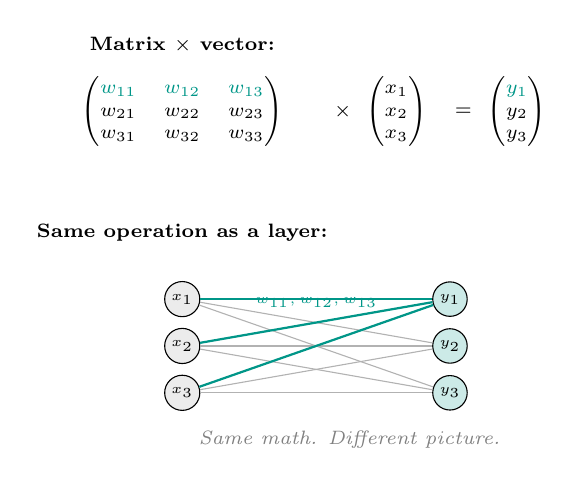
\begin{tikzpicture}[scale=0.85]
        % --- TOP: Matrix times vector ---
        \node[font=\scriptsize] at (0,3.8) {\textbf{Matrix $\times$ vector:}};
        \node[font=\scriptsize] (mat) at (0,2.8) {
          $\begin{pmatrix}
            \textcolor{linalgTeal}{w_{11}} & \textcolor{linalgTeal}{w_{12}} & \textcolor{linalgTeal}{w_{13}}\\
            w_{21} & w_{22} & w_{23}\\
            w_{31} & w_{32} & w_{33}
          \end{pmatrix}$};
        \node[font=\scriptsize] at (2.4,2.8) {$\times$};
        \node[font=\scriptsize] at (3.2,2.8) {
          $\begin{pmatrix}x_1\\x_2\\x_3\end{pmatrix}$};
        \node[font=\scriptsize] at (4.2,2.8) {$=$};
        \node[font=\scriptsize] at (5.0,2.8) {
          $\begin{pmatrix}\textcolor{linalgTeal}{y_1}\\y_2\\y_3\end{pmatrix}$};
        % --- BOTTOM: Same as neural net ---
        \node[font=\scriptsize] at (0,1.0) {\textbf{Same operation as a layer:}};
        % Input nodes
        \node[circle, draw, fill=gray!15, inner sep=1.5pt, font=\tiny]
          (i1) at (0,0) {$x_1$};
        \node[circle, draw, fill=gray!15, inner sep=1.5pt, font=\tiny]
          (i2) at (0,-0.7) {$x_2$};
        \node[circle, draw, fill=gray!15, inner sep=1.5pt, font=\tiny]
          (i3) at (0,-1.4) {$x_3$};
        % Output nodes
        \node[circle, draw, fill=linalgTeal!20, inner sep=1.5pt, font=\tiny]
          (o1) at (4,0) {$y_1$};
        \node[circle, draw, fill=linalgTeal!20, inner sep=1.5pt, font=\tiny]
          (o2) at (4,-0.7) {$y_2$};
        \node[circle, draw, fill=linalgTeal!20, inner sep=1.5pt, font=\tiny]
          (o3) at (4,-1.4) {$y_3$};
        % Connections (weights)
        \draw[thin,gray!60] (i1)--(o1); \draw[thin,gray!60] (i1)--(o2); \draw[thin,gray!60] (i1)--(o3);
        \draw[thin,gray!60] (i2)--(o1); \draw[thin,gray!60] (i2)--(o2); \draw[thin,gray!60] (i2)--(o3);
        \draw[thin,gray!60] (i3)--(o1); \draw[thin,gray!60] (i3)--(o2); \draw[thin,gray!60] (i3)--(o3);
        % Highlight one row
        \draw[thick,linalgTeal] (i1)--(o1);
        \draw[thick,linalgTeal] (i2)--(o1);
        \draw[thick,linalgTeal] (i3)--(o1);
        \node[font=\tiny\itshape,text=linalgTeal] at (2,-0.05) {$w_{11},w_{12},w_{13}$};
        % Caption
        \node[font=\scriptsize\itshape,text=gray] at (2.5,-2.1) {Same math. Different picture.};
      \end{tikzpicture}
    \end{column}
  \end{columns}

  \note{
    ``Every time you send a message to an AI, your words pass through about 96 layers.
    Each layer multiplies your data by a matrix. That's roughly 96 matrix multiplications
    just to generate one word of the response.''
    Emphasize: this is NOT an analogy. Neural network layers ARE matrix multiplications.
    The connection is literal and exact.
    \verifytag{Gauss's elimination method typically dated to c.\,1809--1810.
    Method has earlier precedents in Chinese mathematics (Jiuzhang suanshu).}
  }
\end{frame}

% ----------------------------------------------------------
% Slide 10: The Dot Product -- Measuring Similarity
% ----------------------------------------------------------
\begin{frame}{The Dot Product --- Measuring Similarity}

  \begin{columns}[T]
    \begin{column}{0.47\textwidth}
      \textbf{Recipe} (the dot product in plain language):
      \begin{enumerate}
        \item Take two lists of numbers, same length
        \item Multiply matching entries:\\
              first $\times$ first, second $\times$ second, \ldots
        \item Add up all the products
        \item Result is \textbf{one number}:
      \end{enumerate}

      \vspace{0.3em}
      \begin{center}
        \small
        \begin{tabular}{rl}
          Big positive & $=$ very similar \\
          Near zero & $=$ unrelated \\
          Big negative & $=$ opposites
        \end{tabular}
      \end{center}

      \vspace{0.3em}
      {\footnotesize\colorbox{digitalBlue!8}{\parbox{0.9\linewidth}{%
        \textbf{Formal:}\quad $\mathbf{a} \cdot \mathbf{b}
        = a_1 b_1 + a_2 b_2 + \cdots + a_n b_n$}}}
    \end{column}

    \begin{column}{0.50\textwidth}
      % -- Slide 10: Dot product -- three configurations --
      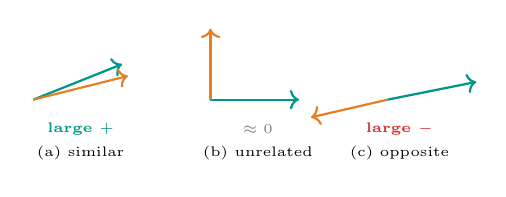
\begin{tikzpicture}[scale=0.75]
        % (a) Same direction
        \begin{scope}[xshift=0cm]
          \draw[->,thick,linalgTeal] (0,0) -- (1.5,0.6);
          \draw[->,thick,accentOrange] (0,0) -- (1.6,0.4);
          \node[font=\tiny\bfseries,text=linalgTeal] at (0.8,-0.5) {large $+$};
          \node[font=\tiny] at (0.8,-0.9) {(a) similar};
        \end{scope}
        % (b) Perpendicular
        \begin{scope}[xshift=3cm]
          \draw[->,thick,linalgTeal] (0,0) -- (1.5,0);
          \draw[->,thick,accentOrange] (0,0) -- (0,1.2);
          \node[font=\tiny\bfseries,text=gray] at (0.8,-0.5) {$\approx 0$};
          \node[font=\tiny] at (0.8,-0.9) {(b) unrelated};
        \end{scope}
        % (c) Opposite
        \begin{scope}[xshift=6cm]
          \draw[->,thick,linalgTeal] (0,0) -- (1.5,0.3);
          \draw[->,thick,accentOrange] (0,0) -- (-1.3,-0.3);
          \node[font=\tiny\bfseries,text=calculusRed] at (0.2,-0.5) {large $-$};
          \node[font=\tiny] at (0.2,-0.9) {(c) opposite};
        \end{scope}
      \end{tikzpicture}

      \vspace{0.2em}
      {\scriptsize\itshape The dot product measures how much two vectors agree.}

      \vspace{0.3em}
      % -- Slide 10: Attention dot-product "it" -> "cat" --
      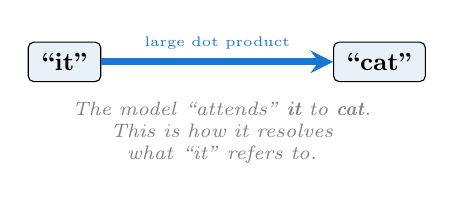
\begin{tikzpicture}
        \node[draw, rounded corners=2pt, fill=probBlue!10, inner sep=4pt,
              font=\small\bfseries] (it) at (0,0) {``it''};
        \node[draw, rounded corners=2pt, fill=probBlue!10, inner sep=4pt,
              font=\small\bfseries] (cat) at (4,0) {``cat''};
        \draw[->,>=stealth, line width=2.5pt, probBlue] (it) -- (cat)
          node[midway, above, font=\tiny] {large dot product};
        \node[font=\scriptsize\itshape, text=gray, text width=4.5cm, align=center]
          at (2,-0.9) {The model ``attends'' \textbf{it} to \textbf{cat}.\\
          This is how it resolves what ``it'' refers to.};
      \end{tikzpicture}
    \end{column}
  \end{columns}

  \note{
    ``The dot product is the simplest possible measure of similarity between two vectors.
    Multiply matching entries and add up. That's it. This tiny operation, repeated
    billions of times, is what lets an LLM understand which words relate to which.''
    Historical: formalized by Gibbs (1880s), implicit in earlier work by Grassmann.
    LLM connection: in the attention mechanism, the dot product of a Query vector and
    a Key vector determines how much ``attention'' one word pays to another.
    Every attention score in every LLM is a dot product.
  }
\end{frame}

% ----------------------------------------------------------
% Slide 11: Cosine Similarity
% ----------------------------------------------------------
\begin{frame}{Cosine Similarity --- Dot Product, Normalized}

  \begin{columns}[T]
    \begin{column}{0.45\textwidth}
      \textbf{Recipe:}
      \begin{enumerate}
        \item Compute the dot product
        \item Divide by the length of each vector
        \item Result is always between $-1$ and $+1$
      \end{enumerate}

      \vspace{0.3em}
      Think of it as: \emph{how much do these two vectors point the same way?}
      (Ignoring how long they are.)

      \vspace{0.5em}
      {\footnotesize\colorbox{digitalBlue!8}{\parbox{0.9\linewidth}{%
        \textbf{Formal:}\quad $\cos(\theta) = \dfrac{\mathbf{a} \cdot \mathbf{b}}%
        {\lvert\mathbf{a}\rvert \;\lvert\mathbf{b}\rvert}$}}}

      \vspace{0.5em}
      \begin{insightbox}
        When you ask an LLM to find ``similar words,'' it computes cosine similarity.
        The math is from the 1880s. The application is from last Tuesday.
      \end{insightbox}
    \end{column}

    \begin{column}{0.52\textwidth}
      % -- Slide 11: Cosine similarity in embedding space --
      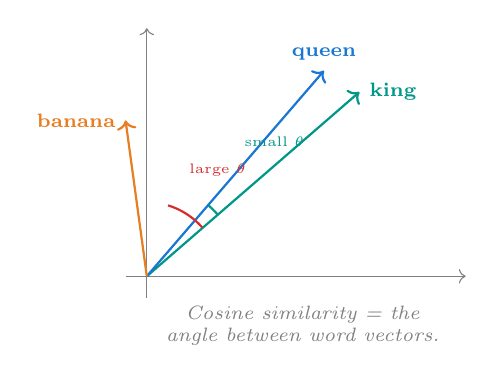
\begin{tikzpicture}[scale=0.9]
        % Axes
        \draw[->,gray,thin] (-0.3,0)--(4.5,0);
        \draw[->,gray,thin] (0,-0.3)--(0,3.5);
        % King vector
        \draw[->,thick,linalgTeal] (0,0) -- (3,2.6)
          node[right,font=\scriptsize\bfseries] {king};
        % Queen vector (close to king)
        \draw[->,thick,probBlue] (0,0) -- (2.5,2.9)
          node[above,font=\scriptsize\bfseries] {queen};
        % Banana vector (far away)
        \draw[->,thick,accentOrange] (0,0) -- (-0.3,2.2)
          node[left,font=\scriptsize\bfseries] {banana};
        % Small angle arc between king and queen
        \draw[linalgTeal, thick] (1.0,0.87) arc[start angle=41, end angle=49, radius=1.33];
        \node[font=\tiny,text=linalgTeal] at (1.8,1.9) {small $\theta$};
        % Large angle arc between king and banana
        \draw[calculusRed, thick] (0.3,1.0) arc[start angle=73, end angle=41, radius=1.05];
        \node[font=\tiny,text=calculusRed] at (1.0,1.5) {large $\theta$};
        % Caption
        \node[font=\scriptsize\itshape, text=gray, text width=4cm, align=center]
          at (2.2,-0.7) {Cosine similarity = the angle between word vectors.};
      \end{tikzpicture}
    \end{column}
  \end{columns}

  \note{
    ``When you ask an LLM to find `similar words,' it computes cosine similarity
    in embedding space. The math is from the 1880s. The application is from
    last Tuesday.''
    This is how search engines, recommendation systems, and LLMs measure
    semantic similarity between pieces of text.
  }
\end{frame}

% ----------------------------------------------------------
% Slide 12: Eigenvalues and Eigenvectors [EXTENDED]
% ----------------------------------------------------------
\begin{frame}{Eigenvalues --- The Natural Modes \hfill {\small\textcolor{gray}{[EXTENDED]}}}

  \begin{columns}[T]
    \begin{column}{0.50\textwidth}
      \begin{personbox}[Leonhard Euler (1707--1783)]{digitalBlue}
        \small
        \textbf{Origin:} Basel, Switzerland / St.\ Petersburg / Berlin\\
        \textbf{Key work:} First encountered eigenvalue-like concepts studying
        vibrating strings and rotating bodies (1740s--1750s).
      \end{personbox}

      \vspace{0.2em}
      \begin{personbox}[Augustin-Louis Cauchy (1789--1857)]{digitalBlue}
        \small
        \textbf{Origin:} Paris, France\\
        \textbf{Key work:} Proved symmetric matrices have real eigenvalues (1829).
      \end{personbox}

      \vspace{0.2em}
      \begin{personbox}[David Hilbert (1862--1943)]{digitalBlue}
        \small
        \textbf{Origin:} K\"onigsberg / G\"ottingen, Germany\\
        \textbf{Key work:} Extended eigenvalue theory to infinite-dimensional
        spaces (spectral theory, early 1900s).
      \end{personbox}
    \end{column}

    \begin{column}{0.47\textwidth}
      % -- Slide 12: Eigenvector visualization --
      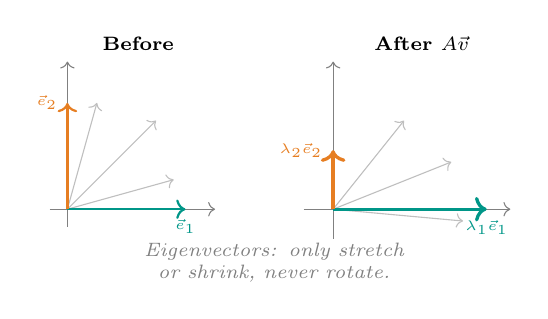
\begin{tikzpicture}[scale=0.75]
        % Before transformation (left)
        \node[font=\scriptsize\bfseries] at (1.2,2.8) {Before};
        \draw[->,gray,thin] (-0.3,0)--(2.5,0);
        \draw[->,gray,thin] (0,-0.3)--(0,2.5);
        \draw[->,thin,gray!50] (0,0)--(1.5,1.5);
        \draw[->,thin,gray!50] (0,0)--(0.5,1.8);
        \draw[->,thin,gray!50] (0,0)--(1.8,0.5);
        \draw[->,thick,linalgTeal] (0,0)--(2.0,0)
          node[below,font=\tiny] {$\vec{e}_1$};
        \draw[->,thick,accentOrange] (0,0)--(0,1.8)
          node[left,font=\tiny] {$\vec{e}_2$};
        % After transformation (right)
        \begin{scope}[xshift=4.5cm]
          \node[font=\scriptsize\bfseries] at (1.5,2.8) {After $A\vec{v}$};
          \draw[->,gray,thin] (-0.5,0)--(3.0,0);
          \draw[->,gray,thin] (0,-0.5)--(0,2.5);
          % Rotated arrows (non-eigenvectors)
          \draw[->,thin,gray!50] (0,0)--(2.0,0.8);
          \draw[->,thin,gray!50] (0,0)--(1.2,1.5);
          \draw[->,thin,gray!50] (0,0)--(2.2,-0.2);
          % Eigenvectors: only stretched, not rotated
          \draw[->,very thick,linalgTeal] (0,0)--(2.6,0)
            node[below,font=\tiny] {$\lambda_1 \vec{e}_1$};
          \draw[->,very thick,accentOrange] (0,0)--(0,1.0)
            node[left,font=\tiny] {$\lambda_2 \vec{e}_2$};
        \end{scope}
        % Caption
        \node[font=\scriptsize\itshape, text=gray, text width=6cm, align=center]
          at (3.5,-0.9) {Eigenvectors: only stretch or shrink, never rotate.};
      \end{tikzpicture}

      \vspace{0.3em}
      {\small\textbf{LLM connection:} Principal Component Analysis (PCA)
        uses eigenvalues to visualize and understand what LLMs learn.
        ``What does this neuron represent?'' --- eigenvalue analysis helps answer.}
    \end{column}
  \end{columns}

  \note{
    This is an [EXTENDED] slide --- can be cut if short on time.
    Eigenvalues reveal the ``natural modes'' of a transformation.
    They appear in dimensionality reduction (PCA), used for understanding
    and compressing neural network representations.
    \verifytag{Euler's eigenvalue work --- verify precise context
    (vibrating membranes vs.\ rotating bodies) and dates.
    Cauchy's 1829 result on symmetric matrices.}
  }
\end{frame}

% ----------------------------------------------------------
% Slide 13: High-Dimensional Spaces -- Where Words Live
% ----------------------------------------------------------
\begin{frame}{High-Dimensional Spaces --- Where Words Live}

  \begin{columns}[T]
    \begin{column}{0.48\textwidth}
      LLMs represent words as vectors in spaces with
      \textbf{hundreds or thousands of dimensions}.

      \vspace{0.3em}
      The math works the same as in 2D or 3D --- we just can't draw it.

      \vspace{0.5em}
      \begin{personbox}[Richard Bellman (1920--1984)]{digitalBlue}
        \small
        \textbf{Origin:} New York City, USA\\
        \textbf{Key work:} Coined ``the curse of dimensionality'' (c.\,1957--1961):
        in high dimensions, data becomes sparse and distances behave
        counterintuitively.
      \end{personbox}
    \end{column}

    \begin{column}{0.49\textwidth}
      % -- Slide 13: Word vector parallelogram --
      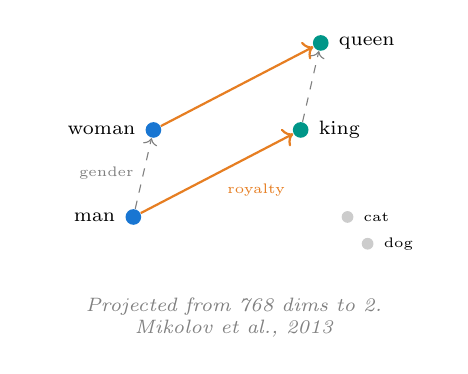
\begin{tikzpicture}[scale=0.85]
        % Word points
        \node[circle, fill=linalgTeal, inner sep=2pt, label={[font=\scriptsize]right:king}]
          (king) at (3.5,2.5) {};
        \node[circle, fill=linalgTeal, inner sep=2pt, label={[font=\scriptsize]right:queen}]
          (queen) at (3.8,3.8) {};
        \node[circle, fill=probBlue, inner sep=2pt, label={[font=\scriptsize]left:man}]
          (man) at (1.0,1.2) {};
        \node[circle, fill=probBlue, inner sep=2pt, label={[font=\scriptsize]left:woman}]
          (woman) at (1.3,2.5) {};
        % Extra words
        \node[circle, fill=gray!40, inner sep=1.5pt, label={[font=\tiny]right:dog}]
          at (4.5,0.8) {};
        \node[circle, fill=gray!40, inner sep=1.5pt, label={[font=\tiny]right:cat}]
          at (4.2,1.2) {};
        % Parallelogram arrows
        \draw[->,thick,accentOrange] (man) -- (king)
          node[midway,below right,font=\tiny] {royalty};
        \draw[->,thick,accentOrange] (woman) -- (queen);
        \draw[->,dashed,gray] (man) -- (woman)
          node[midway,left,font=\tiny] {gender};
        \draw[->,dashed,gray] (king) -- (queen);
        % Caption
        \node[font=\scriptsize\itshape, text=gray, text width=5cm, align=center]
          at (2.5,-0.3) {Projected from 768 dims to 2.\\Mikolov et al., 2013};
      \end{tikzpicture}

      \vspace{0.3em}
      {\small\textbf{Tomas Mikolov} et al.\ demonstrated this with
        \textbf{Word2Vec} (2013) --- word vectors trained on large text corpora
        capture semantic relationships as \emph{linear directions}.}
    \end{column}
  \end{columns}

  \note{
    ``In 768 dimensions, words that mean similar things end up near each other.
    `Dog' is near `puppy.' `Paris' is near `France.' The AI doesn't know what
    these words mean --- it only knows their coordinates. But the coordinates
    capture meaning. Mikolov showed this in 2013 and it stunned the field.''
    \verifytag{Confirm both Mikolov et al.\ 2013 papers: ``Efficient Estimation
    of Word Representations in Vector Space'' (arXiv) and ``Distributed
    Representations of Words and Phrases'' (NeurIPS).}
    \verifytag{Bellman coined ``curse of dimensionality'' --- may be from
    his 1961 book \emph{Adaptive Control Processes}, not 1957. Verify.}
  }
\end{frame}

% ----------------------------------------------------------
% INTERACTIVE MOMENT 1 (after Slide 13)
% ----------------------------------------------------------
\begin{frame}{Quick Experiment --- Word Vector Arithmetic}

  \begin{center}
    {\Large\bfseries\textcolor{aiViolet}{What does this equal?}}

    \vspace{1.5em}
    {\Huge $\underset{\text{king}}{\mathbf{v}} \;-\;
           \underset{\text{man}}{\mathbf{v}} \;+\;
           \underset{\text{woman}}{\mathbf{v}} \;=\; ?$}

    \vspace{1.5em}
    % -- Slide 13i: Reveal -- parallelogram + QUEEN --
    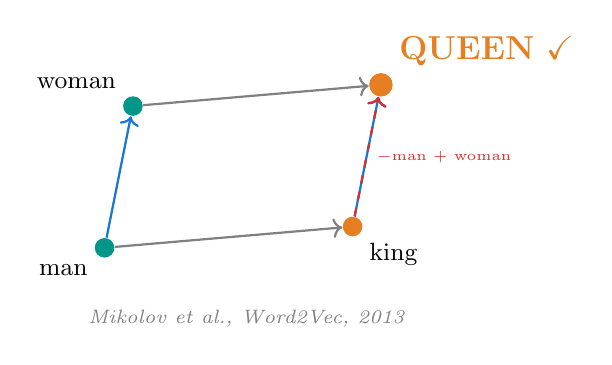
\begin{tikzpicture}[scale=0.9]
      % Parallelogram
      \node[circle, fill=linalgTeal, inner sep=2.5pt,
            label={[font=\small]below left:man}]
        (man) at (0,0) {};
      \node[circle, fill=linalgTeal, inner sep=2.5pt,
            label={[font=\small]above left:woman}]
        (woman) at (0.4,2.0) {};
      \node[circle, fill=accentOrange, inner sep=2.5pt,
            label={[font=\small]below right:king}]
        (king) at (3.5,0.3) {};
      \node[circle, fill=accentOrange, inner sep=3pt,
            label={[font=\large\bfseries,text=accentOrange]above right:QUEEN \checkmark}]
        (queen) at (3.9,2.3) {};
      % Arrows
      \draw[->,thick,gray] (man) -- (king);
      \draw[->,thick,gray] (woman) -- (queen);
      \draw[->,thick,probBlue] (man) -- (woman);
      \draw[->,thick,probBlue] (king) -- (queen);
      % Dashed analogy arrow
      \draw[->,dashed,thick,calculusRed] (king) -- (queen)
        node[midway,right,font=\tiny]{$-$man $+$ woman};
      % Attribution
      \node[font=\scriptsize\itshape, text=gray] at (2,-1.0)
        {Mikolov et al., Word2Vec, 2013};
    \end{tikzpicture}
  \end{center}

  \note{
    INTERACTIVE MOMENT 1 (approx.\ 2 minutes).
    Ask students: ``If we take the vector for `king,' subtract the vector for `man,'
    and add the vector for `woman' --- what word's vector do we land nearest to?''
    Let them guess. Collect answers.
    Reveal: ``queen.'' This works because of the geometry of high-dimensional vector
    spaces, as Mikolov's Word2Vec demonstrated in 2013.
    This is not a trick --- it is a mathematical property of the embedding space.
    Grassmann's abstract vector spaces from 1844 make this possible.
  }
\end{frame}

% ----------------------------------------------------------
% Slide 14: From Words to Numbers -- The Embedding
% ----------------------------------------------------------
\begin{frame}{From Words to Numbers --- The Embedding}

  \begin{center}
    % -- Slide 14: Embedding pipeline --
    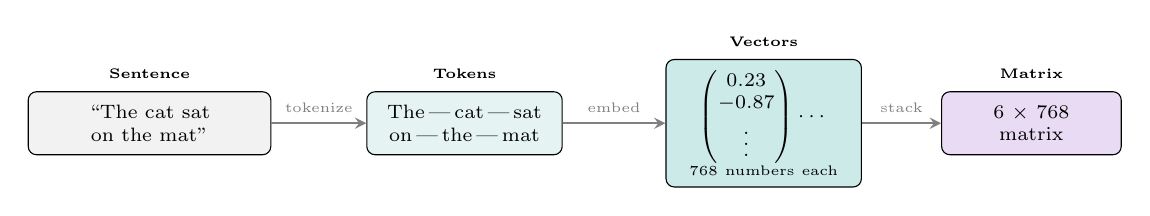
\begin{tikzpicture}[
      bx/.style={draw, rounded corners=3pt, inner sep=4pt,
                 font=\scriptsize, align=center, minimum height=0.8cm},
      arr/.style={->,>=stealth,thick,gray}
    ]
      % Step 1: Sentence
      \node[bx, fill=gray!10, text width=2.8cm] (sent) at (0,0)
        {``The cat sat\\on the mat''};
      \node[font=\tiny\bfseries, above=1pt of sent] {Sentence};
      % Step 2: Tokens
      \node[bx, fill=linalgTeal!10, text width=2.2cm] (tok) at (4,0)
        {The\,|\,cat\,|\,sat\\on\,|\,the\,|\,mat};
      \node[font=\tiny\bfseries, above=1pt of tok] {Tokens};
      % Step 3: Vectors
      \node[bx, fill=linalgTeal!20, text width=2.2cm] (vec) at (7.8,0)
        {$\begin{pmatrix}0.23\\-0.87\\\vdots\end{pmatrix} \cdots$\\{\tiny 768 numbers each}};
      \node[font=\tiny\bfseries, above=1pt of vec] {Vectors};
      % Step 4: Matrix
      \node[bx, fill=aiViolet!15, text width=2.0cm] (mat) at (11.2,0)
        {$6 \times 768$\\matrix};
      \node[font=\tiny\bfseries, above=1pt of mat] {Matrix};
      % Arrows
      \draw[arr] (sent) -- (tok) node[midway,above,font=\tiny] {tokenize};
      \draw[arr] (tok) -- (vec) node[midway,above,font=\tiny] {embed};
      \draw[arr] (vec) -- (mat) node[midway,above,font=\tiny] {stack};
    \end{tikzpicture}

    \vspace{0.3em}
    {\small\bfseries\textcolor{aiViolet}{Your sentence is now a matrix.}
    Everything that follows is linear algebra.}
  \end{center}

  \vspace{0.3em}
  {\small\textbf{Historical lineage:}
    Grassmann (1844, abstract vector spaces)
    $\to$ Mikolov (2013, Word2Vec learned embeddings)
    $\to$ Modern LLM embedding layers (2017--present, learned jointly with the transformer)}

  \note{
    ``Grassmann imagined abstract spaces with any number of dimensions. Cayley gave
    us matrices. Mikolov showed words could live in those spaces. Now, 170 years after
    Grassmann, your words live in his spaces.''
    Key point: after embedding, the sentence IS a matrix. Every operation that follows
    is a matrix operation. This is the bridge from language to linear algebra.
  }
\end{frame}

% ----------------------------------------------------------
% Slide 15: Attention as Matrix Multiplication (Preview)
% ----------------------------------------------------------
\begin{frame}{Attention as Matrix Multiplication --- A Preview}

  \begin{columns}[T]
    \begin{column}{0.55\textwidth}
      \textbf{The attention recipe} (conceptual pipeline):

      \vspace{0.3em}
      \begin{enumerate}
        \item Start with input matrix $X$ (sentence as matrix)
        \item Multiply by $W_Q$ $\to$ get Queries\\
              {\scriptsize (matrix multiplication --- Cayley)}
        \item Multiply by $W_K$ $\to$ get Keys\\
              {\scriptsize (matrix multiplication --- Cayley)}
        \item Multiply by $W_V$ $\to$ get Values\\
              {\scriptsize (matrix multiplication --- Cayley)}
        \item Scores $=$ dot product of each Query with each Key\\
              {\scriptsize (dot product --- Gibbs, Slide 10)}
        \item Normalize scores with softmax\\
              {\scriptsize (probability --- Section 3)}
        \item Output $=$ scores $\times$ Values
      \end{enumerate}

      \vspace{0.3em}
      {\footnotesize\colorbox{digitalBlue!8}{\parbox{0.92\linewidth}{%
        \textbf{Formal (preview):}\quad
        $\text{Attn} = \text{softmax}\!\left(\frac{QK^T}{\sqrt{d}}\right) V$\\[2pt]
        $K^T$ $=$ ``flip the matrix on its side'' (transpose).
        $\sqrt{d}$ $=$ scaling factor.\\
        We will unpack this fully in Section~9.}}}
    \end{column}

    \begin{column}{0.42\textwidth}
      % -- Slide 15: Attention Q,K,V pipeline --
      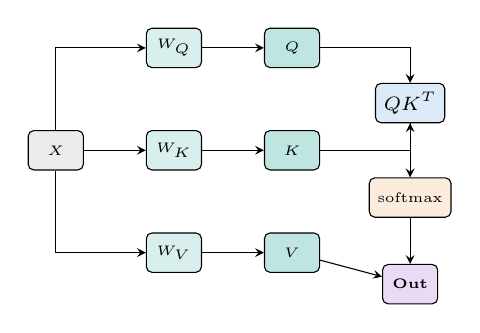
\begin{tikzpicture}[
        bx/.style={draw, rounded corners=2pt, inner sep=3pt,
                   font=\tiny, minimum width=0.7cm, minimum height=0.5cm},
        arr/.style={->,>=stealth,thin}
      ]
        % Input X
        \node[bx, fill=gray!15, font=\tiny\bfseries] (X) at (0,1.5) {$X$};
        % Three parallel paths
        \node[bx, fill=linalgTeal!15] (wq) at (1.5,2.8) {$W_Q$};
        \node[bx, fill=linalgTeal!15] (wk) at (1.5,1.5) {$W_K$};
        \node[bx, fill=linalgTeal!15] (wv) at (1.5,0.2) {$W_V$};
        \node[bx, fill=linalgTeal!25] (Q) at (3.0,2.8) {$Q$};
        \node[bx, fill=linalgTeal!25] (K) at (3.0,1.5) {$K$};
        \node[bx, fill=linalgTeal!25] (V) at (3.0,0.2) {$V$};
        % Arrows: X to W matrices
        \draw[arr] (X) |- (wq);
        \draw[arr] (X) -- (wk);
        \draw[arr] (X) |- (wv);
        % Arrows: W to Q,K,V
        \draw[arr] (wq) -- (Q);
        \draw[arr] (wk) -- (K);
        \draw[arr] (wv) -- (V);
        % Dot product
        \node[bx, fill=probBlue!15] (scores) at (4.5,2.1) {\scriptsize $QK^T$};
        \draw[arr] (Q) -| (scores);
        \draw[arr] (K) -| (scores);
        % Softmax
        \node[bx, fill=accentOrange!15] (sm) at (4.5,0.9) {\tiny softmax};
        \draw[arr] (scores) -- (sm);
        % Times V
        \node[bx, fill=aiViolet!15, font=\tiny\bfseries] (out) at (4.5,-0.2) {Out};
        \draw[arr] (sm) -- (out);
        \draw[arr] (V) -- (out);
      \end{tikzpicture}
    \end{column}
  \end{columns}

  \note{
    ``The `attention' mechanism --- the thing that lets an AI understand context ---
    is three matrix multiplications, a dot product, and a softmax. That's it.
    The math was all invented by the 1880s. The architecture was invented in 2017.''
    This is a PREVIEW. We return to attention in detail in Section 9.
    The point: show students early that ``attention'' is not magic --- it is the
    linear algebra they just learned.
    Do NOT let students get stuck on the formal equation. The conceptual pipeline
    is what matters here.
  }
\end{frame}

% ----------------------------------------------------------
% Slide 16: Convergence Diagram Update -- Linear Algebra
% ----------------------------------------------------------
\begin{frame}{Building the Diagram --- Linear Algebra Complete}

  \begin{columns}[T]
    \begin{column}{0.55\textwidth}
      \begin{center}
        \visualplaceholder[6.5cm]{CONVERGENCE DIAGRAM -- VARIANT 1 (figures/convergence-1.pdf).
          Node (1) ``Linear Algebra'' lit in linalgTeal with solid arrow to center.
          Label: ``Matrix multiplication = neural network layers.''
          Nodes (2)--(10) remain gray with dashed arrows.
          Central node still ``?'' in gray.}
      \end{center}
    \end{column}

    \begin{column}{0.42\textwidth}
      \textbf{Summary --- who built the skeleton:}

      \vspace{0.3em}
      {\small
      \begin{tabular}{@{}rl@{}}
        1843 & Hamilton --- quaternions \\
        1844 & Grassmann --- vector spaces \\
        1850 & Sylvester --- named ``matrix'' \\
        1858 & Cayley --- matrix theory \\
        1880s & Gibbs/Heaviside --- notation \\
        1809+ & Gauss --- elimination \\
        2013 & Mikolov --- Word2Vec \\
      \end{tabular}}

      \vspace{0.5em}
      \begin{insightbox}
        Every layer of an LLM is a matrix multiplication.
        Every attention score is a dot product.
        The math of 1850 is the engine of 2026.
      \end{insightbox}
    \end{column}
  \end{columns}

  \note{
    Transition: ``Now we have the skeleton. But a skeleton doesn't move. For that,
    we need calculus.''
    Recap all six mathematicians and Mikolov. Emphasize the time span:
    from Grassmann's ignored 1844 paper to the core of every modern LLM.
    Connection arrow: ``Every layer of an LLM is a matrix multiplication.
    Every attention score is a dot product. The math of 1850 is the engine of 2026.''
  }
\end{frame}


% ============================================================
% SECTION 2: CALCULUS & OPTIMIZATION -- "How Neural Networks Learn"
% Slides 17-25
% ============================================================
\section{Calculus \& Optimization}

% ----------------------------------------------------------
% Slide 17: Section Divider
% ----------------------------------------------------------
{
\setbeamercolor{background canvas}{bg=enlightenmentTeal}
\begin{frame}[plain]
  \centering
  \vspace{1.5cm}
  \textcolor{white}{\Huge\bfseries Calculus \& Optimization}\\[0.6em]
  \textcolor{white!80}{\large How Neural Networks Learn}\\[1em]
  \textcolor{white!60}{\normalsize c.\,250 BCE -- 1986}\\[1.5em]
  \textcolor{white!70}{\itshape``A neural network learns by rolling downhill
    on a landscape made of calculus.''}

  \note{
    Section transition. Without calculus, you can BUILD a neural network but you
    cannot TRAIN it. Calculus provides the learning algorithm.
    Timeline: from Archimedes' proto-calculus (c.\,250 BCE) to Rumelhart, Hinton,
    and Williams' backpropagation paper (1986).
    Convergence diagram: Section 2 node pulsing.
  }
\end{frame}
}

% ----------------------------------------------------------
% Slide 18: Roots in Antiquity -- Archimedes
% ----------------------------------------------------------
\begin{frame}{Roots in Antiquity --- Archimedes and Infinitesimals}

  \begin{columns}[T]
    \begin{column}{0.50\textwidth}
      \begin{personbox}[Archimedes of Syracuse]{enlightenmentTeal}
        \small
        \textbf{Origin:} Syracuse, Sicily\\
        \textbf{Key work:} The ``method of exhaustion'' --- calculated areas and
        volumes by approximating with ever-finer polygons.\\[3pt]
        His lost \emph{Method} manuscript, rediscovered in 1906 in the
        Archimedes Palimpsest, shows he used infinitesimal reasoning
        more explicitly than previously known.
      \end{personbox}

      \vspace{0.5em}
      \begin{insightbox}
        The core idea of calculus: approximate with simple pieces, take the limit.
        Archimedes had this 1,900 years before Newton.
      \end{insightbox}
    \end{column}

    \begin{column}{0.47\textwidth}
      % -- Slide 18: Method of exhaustion --
      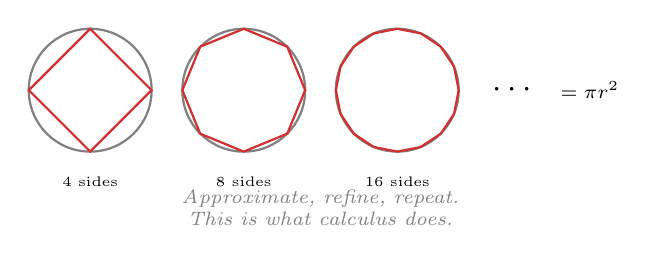
\begin{tikzpicture}[scale=0.65]
        % Circle 1: inscribed square
        \begin{scope}[xshift=0cm]
          \draw[thick,gray] (0,0) circle(1.2);
          \draw[thick,calculusRed] (1.2,0)--(0,1.2)--(-1.2,0)--(0,-1.2)--cycle;
          \node[font=\tiny,below] at (0,-1.5) {4 sides};
        \end{scope}
        % Circle 2: inscribed octagon
        \begin{scope}[xshift=3cm]
          \draw[thick,gray] (0,0) circle(1.2);
          \draw[thick,calculusRed]
            (1.2,0)--(0.85,0.85)--(0,1.2)--(-0.85,0.85)
            --(-1.2,0)--(-0.85,-0.85)--(0,-1.2)--(0.85,-0.85)--cycle;
          \node[font=\tiny,below] at (0,-1.5) {8 sides};
        \end{scope}
        % Circle 3: inscribed 16-gon (approximate with smoother polygon)
        \begin{scope}[xshift=6cm]
          \draw[thick,gray] (0,0) circle(1.2);
          \draw[thick,calculusRed]
            (1.2,0)--(1.11,0.46)--(0.85,0.85)--(0.46,1.11)
            --(0,1.2)--(-0.46,1.11)--(-0.85,0.85)--(-1.11,0.46)
            --(-1.2,0)--(-1.11,-0.46)--(-0.85,-0.85)--(-0.46,-1.11)
            --(0,-1.2)--(0.46,-1.11)--(0.85,-0.85)--(1.11,-0.46)--cycle;
          \node[font=\tiny,below] at (0,-1.5) {16 sides};
        \end{scope}
        % Ellipsis
        \node[font=\large] at (8.3,0) {$\cdots$};
        % Arrow
        \node[font=\scriptsize,right] at (9,0) {$= \pi r^2$};
        % Caption
        \node[font=\scriptsize\itshape, text=gray, text width=5cm, align=center]
          at (4.5,-2.3) {Approximate, refine, repeat.\\This is what calculus does.};
      \end{tikzpicture}
    \end{column}
  \end{columns}

  \note{
    ``Archimedes was doing proto-calculus in the 3rd century BCE,
    1,900 years before Newton.''
    The Archimedes Palimpsest was rediscovered in 1906 --- a medieval prayer book
    written over his mathematical manuscripts. Modern imaging technology revealed
    the hidden text, showing more sophisticated infinitesimal reasoning than
    historians had expected.
  }
\end{frame}

% ----------------------------------------------------------
% Slide 19: The Derivative -- Measuring Change
% ----------------------------------------------------------
\begin{frame}{The Derivative --- Measuring Change}

  \begin{columns}[T]
    \begin{column}{0.48\textwidth}
      \begin{personbox}[Pierre de Fermat (1601--1665)]{enlightenmentTeal}
        \small
        \textbf{Origin:} Beaumont-de-Lomagne, France\\
        \textbf{Key work:} Method for tangent lines (c.\,1636--1638);
        found maxima and minima by setting a difference quotient to zero.
      \end{personbox}

      \vspace{0.2em}
      \begin{personbox}[Isaac Newton (1642--1726/27)]{enlightenmentTeal}
        \small
        \textbf{Origin:} Woolsthorpe, England\\
        \textbf{Key work:} ``Method of fluxions'' (c.\,1665--1666) ---
        rates of change for physics.
      \end{personbox}

      \vspace{0.2em}
      \begin{personbox}[Gottfried Wilhelm Leibniz (1646--1716)]{enlightenmentTeal}
        \small
        \textbf{Origin:} Leipzig, Germany\\
        \textbf{Key work:} Independently developed calculus (published 1684--1686)
        with the $dy/dx$ notation we still use today.
      \end{personbox}
    \end{column}

    \begin{column}{0.49\textwidth}
      % -- Slide 19: Three derivative notations --
      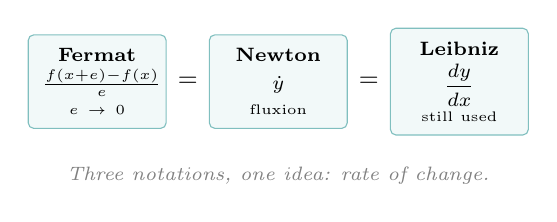
\begin{tikzpicture}
        \node[draw=enlightenmentTeal!50, fill=enlightenmentTeal!5,
              rounded corners=2pt, inner sep=5pt, text width=1.4cm,
              align=center, font=\scriptsize]
          (fer) at (0,0) {\textbf{Fermat}\\[2pt]$\frac{f(x+e)-f(x)}{e}$\\[1pt]{\tiny $e\to 0$}};
        \node[draw=enlightenmentTeal!50, fill=enlightenmentTeal!5,
              rounded corners=2pt, inner sep=5pt, text width=1.4cm,
              align=center, font=\scriptsize]
          (new) at (2.3,0) {\textbf{Newton}\\[2pt]$\dot{y}$\\[1pt]{\tiny fluxion}};
        \node[draw=enlightenmentTeal!50, fill=enlightenmentTeal!5,
              rounded corners=2pt, inner sep=5pt, text width=1.4cm,
              align=center, font=\scriptsize]
          (lei) at (4.6,0) {\textbf{Leibniz}\\[2pt]$\dfrac{dy}{dx}$\\[1pt]{\tiny still used}};
        % Equals signs
        \node[font=\small] at (1.15,0) {$=$};
        \node[font=\small] at (3.45,0) {$=$};
        % Caption
        \node[font=\scriptsize\itshape, text=gray] at (2.3,-1.2)
          {Three notations, one idea: rate of change.};
      \end{tikzpicture}

      \vspace{0.3em}
      % -- Slide 19: Curve with tangent line --
      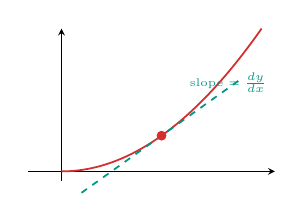
\begin{tikzpicture}[scale=0.8]
        \begin{axis}[
          width=5.5cm, height=4cm,
          axis lines=middle,
          ticks=none,
          xmin=-0.5, xmax=3.2, ymin=-0.3, ymax=4.5,
          clip=false
        ]
          % Curve f(x) = x^2/2
          \addplot[domain=0:3, smooth, thick, calculusRed, samples=40] {x*x/2};
          % Tangent line at x=1.5: f(1.5)=1.125, f'(1.5)=1.5
          \addplot[domain=0.3:2.7, thick, linalgTeal, dashed] {1.5*(x-1.5)+1.125};
          % Point of tangency
          \addplot[only marks, mark=*, mark size=2pt, calculusRed] coordinates {(1.5,1.125)};
          % Label
          \node[font=\tiny, text=linalgTeal] at (axis cs:2.5,2.8) {slope $= \frac{dy}{dx}$};
        \end{axis}
      \end{tikzpicture}

      \vspace{0.1em}
      {\scriptsize\itshape The derivative = the slope of this line.}

      \vspace{0.3em}
      {\small\textbf{LLM connection:} Training means computing
        derivatives of the error w.r.t.\ \emph{every} weight ---
        billions of weights, billions of derivatives, millions of times.}
    \end{column}
  \end{columns}

  \note{
    ``Newton and Leibniz famously fought over who invented calculus. Fermat was
    doing something similar decades earlier. None of them imagined that 300 years
    later, derivatives would be computed trillions of times to train a chatbot.''
    Note: Fermat also appears in Section 3 (Probability) with Pascal.
    When he comes up again, point out: ``Fermat again! He contributed to both
    calculus and probability --- two separate pillars of the LLM.''
  }
\end{frame}

% ----------------------------------------------------------
% Slide 20: The Chain Rule -- The Key to Backpropagation
% ----------------------------------------------------------
\begin{frame}{The Chain Rule --- The Key to Backpropagation}

  \begin{columns}[T]
    \begin{column}{0.47\textwidth}
      \textbf{Recipe} (the chain rule in plain language):

      \vspace{0.3em}
      If $y$ depends on $u$ and $u$ depends on $x$\ldots

      \vspace{0.2em}
      To find how much $x$ affected $y$ through the chain,
      \alert{multiply the effects at each step}.

      \vspace{0.5em}
      {\footnotesize\colorbox{enlightenmentTeal!8}{\parbox{0.92\linewidth}{%
        \textbf{Formal:}\quad
        $\dfrac{dy}{dx} = \dfrac{dy}{du} \cdot \dfrac{du}{dx}$\\[4pt]
        Leibniz's notation makes this look almost obvious ---
        the $du$'s ``cancel.'' (They don't really, but the intuition helps.)}}}

      \vspace{0.5em}
      \begin{insightbox}
        Backpropagation uses the chain rule to figure out which weights
        to blame for the error.
      \end{insightbox}
    \end{column}

    \begin{column}{0.50\textwidth}
      % -- Slide 20: Chain rule -- math + neural net --
      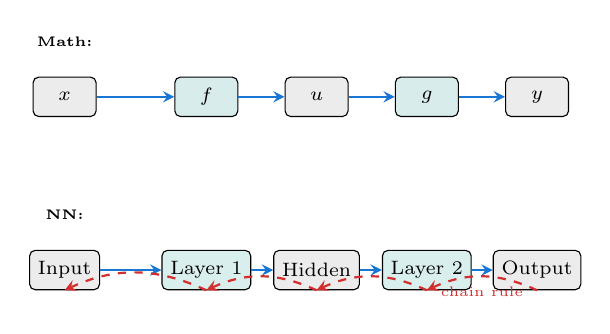
\begin{tikzpicture}[
        bx/.style={draw, rounded corners=2pt, inner sep=3pt,
                   font=\scriptsize, minimum width=0.8cm, minimum height=0.5cm},
        arr/.style={->,>=stealth,thick}
      ]
        % TOP ROW: Math version
        \node[font=\tiny\bfseries] at (0,3.2) {Math:};
        \node[bx, fill=gray!15] (x1) at (0,2.5) {$x$};
        \node[bx, fill=enlightenmentTeal!15] (f) at (1.8,2.5) {$f$};
        \node[bx, fill=gray!15] (u) at (3.2,2.5) {$u$};
        \node[bx, fill=enlightenmentTeal!15] (g) at (4.6,2.5) {$g$};
        \node[bx, fill=gray!15] (y1) at (6.0,2.5) {$y$};
        \draw[arr,probBlue] (x1)--(f);
        \draw[arr,probBlue] (f)--(u);
        \draw[arr,probBlue] (u)--(g);
        \draw[arr,probBlue] (g)--(y1);
        % BOTTOM ROW: Neural net version
        \node[font=\tiny\bfseries] at (0,1.0) {NN:};
        \node[bx, fill=gray!15] (xi) at (0,0.3) {Input};
        \node[bx, fill=linalgTeal!15] (l1) at (1.8,0.3) {Layer 1};
        \node[bx, fill=gray!15] (h) at (3.2,0.3) {Hidden};
        \node[bx, fill=linalgTeal!15] (l2) at (4.6,0.3) {Layer 2};
        \node[bx, fill=gray!15] (o) at (6.0,0.3) {Output};
        % Forward arrows (blue)
        \draw[arr,probBlue] (xi)--(l1);
        \draw[arr,probBlue] (l1)--(h);
        \draw[arr,probBlue] (h)--(l2);
        \draw[arr,probBlue] (l2)--(o);
        % Backward arrows (red)
        \draw[arr,calculusRed,dashed] (o.south) to[bend right=25] node[below,font=\tiny,text=calculusRed]{chain rule} (l2.south);
        \draw[arr,calculusRed,dashed] (l2.south) to[bend right=25] (h.south);
        \draw[arr,calculusRed,dashed] (h.south) to[bend right=25] (l1.south);
        \draw[arr,calculusRed,dashed] (l1.south) to[bend right=25] (xi.south);
      \end{tikzpicture}
    \end{column}
  \end{columns}

  \note{
    ``Backpropagation --- the algorithm that trains every neural network --- is
    `just' the chain rule applied over and over, layer by layer, backwards through
    the network. It's calculus class, running at scale.''
    Historical: the chain rule was implicit in Leibniz; made explicit by various
    18th--19th century mathematicians. No single ``inventor.''
    \verifytag{The precise attribution of the chain rule is diffuse --- Leibniz,
    Euler, and others all used it.}
  }
\end{frame}

% ----------------------------------------------------------
% Slide 21: Gradient Descent [EXTENDED]
% ----------------------------------------------------------
\begin{frame}{Gradient Descent --- Rolling Downhill \hfill {\small\textcolor{gray}{[EXTENDED]}}}

  \begin{columns}[T]
    \begin{column}{0.45\textwidth}
      \begin{personbox}[Augustin-Louis Cauchy (1789--1857)]{enlightenmentTeal}
        \small
        \textbf{Origin:} Paris, France\\
        \textbf{Key work:} Published the first description of the method of
        steepest descent (1847), \emph{M\'ethode g\'en\'erale pour la
        r\'esolution des syst\`emes d'\'equations simultan\'ees}.
      \end{personbox}

      \vspace{0.5em}
      \textbf{Recipe:}
      \begin{enumerate}
        \item Compute the gradient (``which way is uphill?'')
        \item Take a small step in the \alert{opposite} direction
        \item Repeat
      \end{enumerate}

      \vspace{0.3em}
      {\small Cauchy was solving equations, not training neural networks.\\
       But the algorithm is the same.}
    \end{column}

    \begin{column}{0.52\textwidth}
      % -- Slide 21: Gradient descent as 2D contour map --
      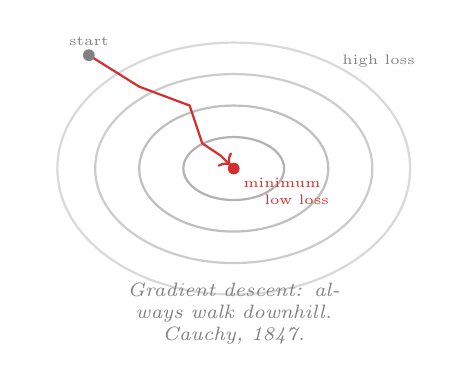
\begin{tikzpicture}[scale=0.8]
        % Contour ellipses (loss landscape top-down view)
        \draw[gray!30, thick] (2.5,1.5) ellipse(2.8 and 2.0);
        \draw[gray!40, thick] (2.5,1.5) ellipse(2.2 and 1.5);
        \draw[gray!50, thick] (2.5,1.5) ellipse(1.5 and 1.0);
        \draw[gray!60, thick] (2.5,1.5) ellipse(0.8 and 0.5);
        % Minimum label
        \node[circle, fill=calculusRed, inner sep=1.5pt] (min) at (2.5,1.5) {};
        \node[font=\tiny, below right, text=calculusRed] at (2.5,1.5) {minimum};
        % Gradient descent path (zigzag)
        \draw[->,thick,calculusRed]
          (0.2,3.3) -- (1.0,2.8) -- (1.8,2.5) -- (2.0,1.9) -- (2.3,1.7) -- (2.45,1.55);
        \node[circle, fill=gray, inner sep=1.5pt] at (0.2,3.3) {};
        \node[font=\tiny, above, text=gray] at (0.2,3.3) {start};
        % Labels
        \node[font=\tiny, text=gray] at (4.8,3.2) {high loss};
        \node[font=\tiny, text=calculusRed] at (3.5,1.0) {low loss};
        % Caption
        \node[font=\scriptsize\itshape, text=gray, text width=5cm, align=center]
          at (2.5,-0.8) {Gradient descent: always walk downhill.\\Cauchy, 1847.};
      \end{tikzpicture}
    \end{column}
  \end{columns}

  \note{
    This is an [EXTENDED] slide --- can be cut, covered verbally in the backprop slide.
    ``Cauchy described this in 1847 to solve equations. 170 years later, it's how
    every LLM on Earth is trained. The error is the height. The gradient tells you
    which way is downhill. You take a step. Repeat a billion times.''
    \verifytag{Cauchy 1847 paper on steepest descent --- confirm exact title and year.}
  }
\end{frame}

% ----------------------------------------------------------
% Slide 22: Backpropagation
% ----------------------------------------------------------
\begin{frame}{Backpropagation --- The Algorithm That Changed Everything}

  \begin{columns}[T]
    \begin{column}{0.50\textwidth}
      \begin{personbox}[{Seppo Linnainmaa (b.\,1945)}]{enlightenmentTeal}
        \small
        \textbf{Origin:} Finland\\
        \textbf{Key work:} Published automatic differentiation in his
        Master's thesis (1970, University of Helsinki) --- the mathematical
        core of backpropagation.
      \end{personbox}

      \vspace{0.2em}
      \begin{personbox}[Rumelhart/Hinton/Williams (1986)]{enlightenmentTeal}
        \small
        \textbf{David Rumelhart} (1942--2011, USA)\\
        \textbf{Geoffrey Hinton} (b.\,1947, London, UK/Canada)\\
        \textbf{Ronald Williams} (USA)\\[3pt]
        Published ``Learning representations by back-propagating errors''
        (1986, \emph{Nature}). Demonstrated backprop could train
        multi-layer networks. Reignited the field.\\[3pt]
        \textbf{Hinton shared the 2024 Nobel Prize in Physics}
        with John Hopfield for foundational work enabling machine learning.
      \end{personbox}
    \end{column}

    \begin{column}{0.47\textwidth}
      % -- Slide 22: Backpropagation network --
      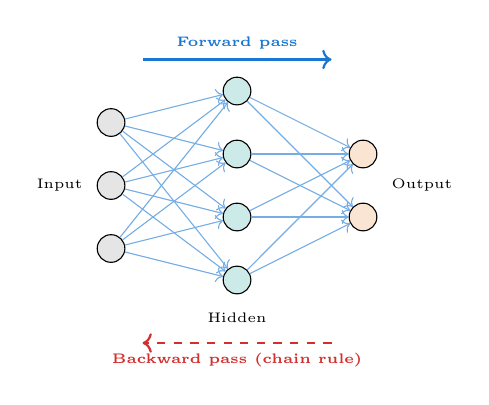
\begin{tikzpicture}[
        neuron/.style={circle, draw, minimum size=10pt, inner sep=0pt, font=\tiny},
        scale=0.8
      ]
        % Input layer (3 nodes)
        \node[neuron, fill=gray!20] (i1) at (0,2.0) {};
        \node[neuron, fill=gray!20] (i2) at (0,1.0) {};
        \node[neuron, fill=gray!20] (i3) at (0,0.0) {};
        \node[font=\tiny,left] at (-0.3,1.0) {Input};
        % Hidden layer (4 nodes)
        \node[neuron, fill=linalgTeal!20] (h1) at (2,2.5) {};
        \node[neuron, fill=linalgTeal!20] (h2) at (2,1.5) {};
        \node[neuron, fill=linalgTeal!20] (h3) at (2,0.5) {};
        \node[neuron, fill=linalgTeal!20] (h4) at (2,-0.5) {};
        \node[font=\tiny] at (2,-1.1) {Hidden};
        % Output layer (2 nodes)
        \node[neuron, fill=accentOrange!20] (o1) at (4,1.5) {};
        \node[neuron, fill=accentOrange!20] (o2) at (4,0.5) {};
        \node[font=\tiny,right] at (4.3,1.0) {Output};
        % Forward connections (blue, thin)
        \draw[->,thin,probBlue!60] (i1)--(h1); \draw[->,thin,probBlue!60] (i1)--(h2);
        \draw[->,thin,probBlue!60] (i1)--(h3); \draw[->,thin,probBlue!60] (i1)--(h4);
        \draw[->,thin,probBlue!60] (i2)--(h1); \draw[->,thin,probBlue!60] (i2)--(h2);
        \draw[->,thin,probBlue!60] (i2)--(h3); \draw[->,thin,probBlue!60] (i2)--(h4);
        \draw[->,thin,probBlue!60] (i3)--(h1); \draw[->,thin,probBlue!60] (i3)--(h2);
        \draw[->,thin,probBlue!60] (i3)--(h3); \draw[->,thin,probBlue!60] (i3)--(h4);
        \draw[->,thin,probBlue!60] (h1)--(o1); \draw[->,thin,probBlue!60] (h1)--(o2);
        \draw[->,thin,probBlue!60] (h2)--(o1); \draw[->,thin,probBlue!60] (h2)--(o2);
        \draw[->,thin,probBlue!60] (h3)--(o1); \draw[->,thin,probBlue!60] (h3)--(o2);
        \draw[->,thin,probBlue!60] (h4)--(o1); \draw[->,thin,probBlue!60] (h4)--(o2);
        % Forward label
        \draw[->,thick,probBlue] (0.5,3.0) -- (3.5,3.0)
          node[midway,above,font=\tiny\bfseries] {Forward pass};
        % Backward label
        \draw[->,thick,calculusRed,dashed] (3.5,-1.5) -- (0.5,-1.5)
          node[midway,below,font=\tiny\bfseries] {Backward pass (chain rule)};
      \end{tikzpicture}

      \vspace{0.3em}
      {\small\textbf{Timeline:}}

      \vspace{0.2em}
      {\footnotesize
      \begin{tabular}{@{}rl@{}}
        1847 & Cauchy --- steepest descent \\
        1970 & Linnainmaa --- auto.\ differentiation \\
        1986 & Rumelhart/Hinton/Williams --- backprop \\
        2024 & Hinton --- Nobel Prize in Physics \\
      \end{tabular}}
    \end{column}
  \end{columns}

  \note{
    ``Linnainmaa figured out the algorithm in 1970. Rumelhart, Hinton, and Williams
    showed it could train neural networks in 1986. Hinton shared the Nobel Prize
    in Physics in 2024 with John Hopfield for foundational work enabling machine
    learning with artificial neural networks.''
    \verifytag{Linnainmaa's 1970 thesis --- some sources describe it as reverse-mode
    automatic differentiation. Others credit earlier related ideas (Bryson, Dreyfus,
    Kelley in the 1960s, control theory). Present Linnainmaa as key formalization
    but note broader lineage.}
    \verifytag{Nobel Prize 2024 --- Hinton and Hopfield shared the Nobel Prize
    in Physics 2024. Confirm exact citation wording.}
  }
\end{frame}

% ----------------------------------------------------------
% Slide 23: Stochastic Gradient Descent
% ----------------------------------------------------------
\begin{frame}{Stochastic Gradient Descent --- Learning from Samples}

  \begin{columns}[T]
    \begin{column}{0.45\textwidth}
      \begin{personbox}[Robbins \& Monro (1951)]{enlightenmentTeal}
        \small
        \textbf{Herbert Robbins} (1915--2001, New Castle, PA, USA)\\
        \textbf{Sutton Monro} (1920--1995, USA)\\[3pt]
        Published the Robbins--Monro algorithm (1951) --- the first
        stochastic approximation method.
        The theoretical foundation for SGD.
      \end{personbox}

      \vspace{0.5em}
      \begin{insightbox}
        Every LLM you have ever used was trained with some variant of SGD.
        The Robbins--Monro paper from 1951 is running inside every AI lab today.
      \end{insightbox}
    \end{column}

    \begin{column}{0.52\textwidth}
      % -- Slide 23: Full GD vs SGD comparison --
      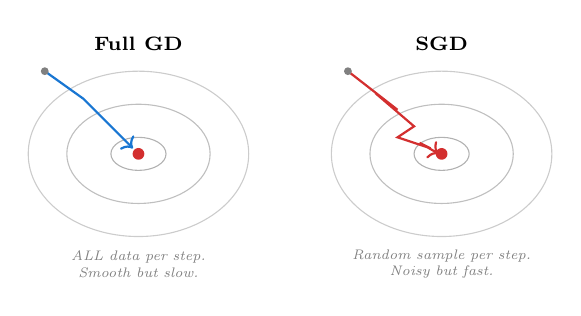
\begin{tikzpicture}[scale=0.7]
        % LEFT: Full GD
        \begin{scope}[xshift=0cm]
          \node[font=\scriptsize\bfseries] at (2,3.5) {Full GD};
          % Contours
          \draw[gray!40] (2,1.5) ellipse(2.0 and 1.5);
          \draw[gray!50] (2,1.5) ellipse(1.3 and 0.9);
          \draw[gray!60] (2,1.5) ellipse(0.5 and 0.3);
          % Smooth path
          \draw[->,thick,probBlue] (0.3,3.0) -- (1.0,2.5) -- (1.5,2.0) -- (1.9,1.6);
          \node[circle,fill=gray,inner sep=1pt] at (0.3,3.0) {};
          \node[circle,fill=calculusRed,inner sep=1.5pt] at (2,1.5) {};
          \node[font=\tiny\itshape, text=gray, text width=2.5cm, align=center]
            at (2,-0.5) {ALL data per step.\\Smooth but slow.};
        \end{scope}
        % RIGHT: SGD
        \begin{scope}[xshift=5.5cm]
          \node[font=\scriptsize\bfseries] at (2,3.5) {SGD};
          % Contours
          \draw[gray!40] (2,1.5) ellipse(2.0 and 1.5);
          \draw[gray!50] (2,1.5) ellipse(1.3 and 0.9);
          \draw[gray!60] (2,1.5) ellipse(0.5 and 0.3);
          % Noisy zigzag path
          \draw[->,thick,calculusRed]
            (0.3,3.0) -- (1.2,2.3) -- (0.8,2.6) -- (1.5,2.0)
            -- (1.2,1.8) -- (1.8,1.6) -- (1.6,1.7) -- (1.95,1.5);
          \node[circle,fill=gray,inner sep=1pt] at (0.3,3.0) {};
          \node[circle,fill=calculusRed,inner sep=1.5pt] at (2,1.5) {};
          \node[font=\tiny\itshape, text=gray, text width=2.5cm, align=center]
            at (2,-0.5) {Random sample per step.\\Noisy but fast.};
        \end{scope}
      \end{tikzpicture}
    \end{column}
  \end{columns}

  \note{
    ``Training GPT-4 used trillions of tokens. You can't compute the gradient
    on all of them at once. SGD says: just grab a random batch, compute the
    gradient on that, take a step, repeat. It's noisy, but it works. And it's fast.''
    LLM connection: every LLM ever deployed was trained with some variant of SGD.
    \verifytag{Monro's dates (1920--1995) and birthplace --- verify.}
  }
\end{frame}

% ----------------------------------------------------------
% Slide 24: The Loss Landscape -- A Visual Tour
% ----------------------------------------------------------
\begin{frame}{The Loss Landscape --- A Visual Tour}

  \begin{center}
    \visualplaceholder[12cm]{3D LOSS LANDSCAPE (to be generated as figures/loss-landscape.pdf via Python/matplotlib or pgfplots standalone).
      Style: Li et al., 2018 ``Visualizing the Loss Landscape of Neural Nets.''
      Surface: 3D plot of $f(x,y) = 0.5(x^2+y^2) + 3\exp(-2((x-1)^2+(y+1)^2)) - \exp(-3((x+1.5)^2+(y-0.5)^2))$
      or similar multi-modal surface.
      Labeled annotations:
      (A) ``Global minimum'' -- deepest valley, green marker
      (B) ``Local minimum'' -- secondary valley, yellow marker
      (C) ``Saddle point'' -- flat ridge, gray marker
      (D) ``SGD path'' -- noisy red trajectory from random start to global min
      Colormap: viridis or coolwarm. View angle: 30\textdegree{} elevation.}
  \end{center}

  \vspace{-0.3em}
  {\small\centering\textcolor{gray}{This is what training an LLM looks like
    mathematically. The landscape has \emph{billions} of dimensions ---
    we can only visualize a 2D slice.}\par}

  \note{
    ``This is what training an LLM looks like mathematically. You start at a random
    point on this landscape and try to find the lowest valley. The landscape has
    billions of dimensions --- we can only visualize a 2D slice.''
    The ``loss'' measures how wrong the network's predictions are.
    Training = finding the lowest point on this landscape.
    SGD's noisy path actually helps --- it can escape shallow local minima
    that full gradient descent might get stuck in.
  }
\end{frame}

% ----------------------------------------------------------
% Slide 25: Convergence Diagram Update -- Calculus & Optimization
% ----------------------------------------------------------
\begin{frame}{Building the Diagram --- Calculus Complete}

  \begin{columns}[T]
    \begin{column}{0.55\textwidth}
      \begin{center}
        \visualplaceholder[6.5cm]{CONVERGENCE DIAGRAM -- VARIANT 2 (figures/convergence-2.pdf).
          Node (1) ``Linear Algebra'' lit in linalgTeal (from Section 1).
          Node (2) ``Calculus \& Optimization'' now lit in calculusRed.
          Label: ``Gradient descent = how it learns.''
          Nodes (3)--(10) remain gray with dashed arrows.
          Central node still ``?'' in gray.}
      \end{center}
    \end{column}

    \begin{column}{0.42\textwidth}
      \textbf{Summary --- who taught it to learn:}

      \vspace{0.3em}
      {\small
      \begin{tabular}{@{}rl@{}}
        c.\,250 BCE & Archimedes --- proto-calculus \\
        c.\,1636 & Fermat --- tangents, extrema \\
        1665--66 & Newton --- fluxions \\
        1684--86 & Leibniz --- $dy/dx$ notation \\
        1847 & Cauchy --- steepest descent \\
        1951 & Robbins--Monro --- SGD \\
        1970 & Linnainmaa --- auto.\ diff. \\
        1986 & Rumelhart/Hinton/Williams \\
               & \quad --- backpropagation \\
      \end{tabular}}

      \vspace{0.5em}
      \begin{insightbox}
        Gradient descent + backpropagation = the learning algorithm of every LLM.
      \end{insightbox}
    \end{column}
  \end{columns}

  \note{
    Transition: ``The network can now learn. But learn WHAT? It learns to predict
    probability distributions over words. For that, we need probability theory.''
    Connection arrow: ``Gradient descent + backpropagation = the learning algorithm
    of every LLM.''
    This is the end of Session 1 (Slides 1--25). Natural break point.
    ``We now know the skeleton of a neural network and how it learns.
    Next: how does it deal with uncertainty?''
  }
\end{frame}

% --- SESSION 1 BREAK (after Slide 25) ---
\sessionbreak{Session 1 Complete}{``We know the skeleton and how it learns. Next: how does it handle uncertainty?''}

% ---- Part 2: Probability + Information Theory + Logic & Computation ----
% ============================================================
% Part 2: Probability & Statistics, Information Theory,
%         Logic & Computation (Slides 26-48)
% Companion lecture: "The Building Blocks of LLMs"
% This file is \input'ed from the main document.
% ============================================================


% ************************************************************
% SECTION 3: PROBABILITY & STATISTICS (Slides 26-34)
% "The Language of Uncertainty"
% Section color: aiViolet
% ************************************************************
\section{Probability \& Statistics}

% ----------------------------------------------------------
% Slide 26: Section Divider
% ----------------------------------------------------------
{
\setbeamercolor{background canvas}{bg=aiViolet}
\begin{frame}[plain]
  \centering
  \vspace{2cm}
  \textcolor{white}{\Huge\bfseries Probability \& Statistics}\\[0.5em]
  \textcolor{white}{\Huge\bfseries The Language of Uncertainty}\\[1em]
  \textcolor{white!80}{\large 1654--1933}\\[1.5em]
  \textcolor{white!60}{\normalsize Pascal \(\cdot\) Fermat \(\cdot\) Bernoulli \(\cdot\) Bayes \(\cdot\) Kolmogorov \(\cdot\) Fisher \(\cdot\) Shannon \(\cdot\) Boltzmann}

  \note{
    Transition from Section~2: ``The network can now learn. But learn WHAT?
    It learns to predict probability distributions over words.
    For that, we need probability theory.''

    Tagline: An LLM doesn't KNOW the next word. It assigns PROBABILITIES
    to every possible word.

    This section covers \(\sim\)10 minutes.
  }
\end{frame}
}

% ----------------------------------------------------------
% Slide 27: The Birth of Probability -- A Gambling Problem
% ----------------------------------------------------------
\begin{frame}{The Birth of Probability --- A Gambling Problem (1654)}

  \begin{columns}[T]
    \begin{column}{0.48\textwidth}
      \begin{personbox}[Blaise Pascal (1623--1662)]{aiViolet}
        \textbf{Origin:} Clermont-Ferrand, France\\[3pt]
        Mathematician, physicist, philosopher. Co-founded probability
        theory in correspondence with Fermat (1654) about the
        \alert{problem of points}: how to divide stakes in an
        interrupted game of chance.
      \end{personbox}

      \vspace{0.4em}
      \begin{personbox}[Pierre de Fermat (1601--1665)]{aiViolet}
        \textbf{Origin:} Beaumont-de-Lomagne, France\\[3pt]
        His reply to Pascal laid out the counting arguments that
        became \textbf{combinatorial probability}.
      \end{personbox}
    \end{column}

    \begin{column}{0.49\textwidth}
      % Visual: Letter exchange and game tree
      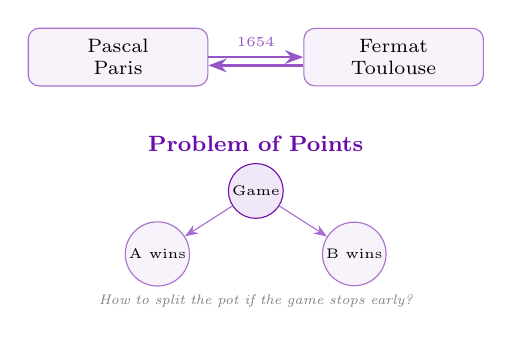
\begin{tikzpicture}[
        letter/.style={draw=aiViolet!60, rounded corners, fill=aiViolet!5,
          text width=2cm, align=center, font=\scriptsize, inner sep=4pt},
        >=Stealth
      ]
        \node[letter] (pascal) at (0,2.5) {Pascal\\Paris};
        \node[letter] (fermat) at (3.5,2.5) {Fermat\\Toulouse};
        \draw[->,thick,aiViolet!70] (pascal.east) -- node[above,font=\tiny] {1654} (fermat.west);
        \draw[<-,thick,aiViolet!70] ([yshift=-3pt]pascal.east) -- ([yshift=-3pt]fermat.west);

        % Simplified game tree
        \node[font=\footnotesize\bfseries,aiViolet] at (1.75,1.4) {Problem of Points};
        \node[circle,draw=aiViolet,fill=aiViolet!10,inner sep=1pt,font=\tiny] (r) at (1.75,0.8) {Game};
        \node[circle,draw=aiViolet!60,fill=aiViolet!5,inner sep=1pt,font=\tiny] (a) at (0.5,0) {A wins};
        \node[circle,draw=aiViolet!60,fill=aiViolet!5,inner sep=1pt,font=\tiny] (b) at (3,0) {B wins};
        \draw[->,aiViolet!60] (r) -- (a);
        \draw[->,aiViolet!60] (r) -- (b);
        \node[font=\tiny\itshape,text=gray,text width=4cm,align=center] at (1.75,-0.6)
          {How to split the pot if the game stops early?};
      \end{tikzpicture}
    \end{column}
  \end{columns}

  \note{
    ``Probability theory was born because a gambler asked Pascal a question
    about how to split the pot in an unfinished dice game. Pascal wrote to
    Fermat. Their letters invented a new branch of mathematics.''

    Fermat again! We saw him in calculus (tangent lines, Slide~19). He
    contributed foundational ideas to TWO separate pillars of the LLM.
  }
\end{frame}

% ----------------------------------------------------------
% Slide 28: From Gambling to Laws -- Bernoulli and Laplace
% ----------------------------------------------------------
\begin{frame}{From Gambling to Laws --- Bernoulli and Laplace}

  \begin{columns}[T]
    \begin{column}{0.5\textwidth}
      \begin{personbox}[Jacob Bernoulli (1655--1705)]{aiViolet}
        \textbf{Origin:} Basel, Switzerland\\[3pt]
        Proved the \alert{law of large numbers} (published posthumously
        in \emph{Ars Conjectandi}, 1713): as you repeat an experiment,
        the observed frequency converges to the true probability.
      \end{personbox}

      \vspace{0.3em}
      \begin{personbox}[Pierre-Simon Laplace (1749--1827)]{aiViolet}
        \textbf{Origin:} Beaumont-en-Auge, France\\[3pt]
        \emph{Th\'eorie analytique des probabilit\'es} (1812)
        systematized the entire field. Popularized Bayes' theorem.
      \end{personbox}
    \end{column}

    \begin{column}{0.47\textwidth}
      % Law of large numbers illustration
      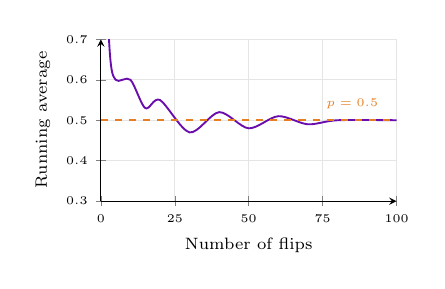
\begin{tikzpicture}[scale=0.85]
        \begin{axis}[
          width=6cm, height=4cm,
          xlabel={\scriptsize Number of flips},
          ylabel={\scriptsize Running average},
          ymin=0.3, ymax=0.7,
          xmin=0, xmax=100,
          ytick={0.3,0.4,0.5,0.6,0.7},
          xtick={0,25,50,75,100},
          grid=major,
          grid style={gray!20},
          axis lines=left,
          tick label style={font=\tiny},
          label style={font=\tiny},
        ]
          % Simulated convergence to 0.5
          \addplot[aiViolet, thick, smooth] coordinates {
            (1,1.0) (3,0.67) (5,0.6) (10,0.6) (15,0.53)
            (20,0.55) (30,0.47) (40,0.52) (50,0.48)
            (60,0.51) (70,0.49) (80,0.50) (100,0.50)
          };
          \draw[dashed, accentOrange, thick] (axis cs:0,0.5) -- (axis cs:100,0.5);
          \node[font=\tiny, accentOrange] at (axis cs:85,0.54) {$p = 0.5$};
        \end{axis}
      \end{tikzpicture}

      \vspace{0.3em}
      \begin{insightbox}
        Why do LLMs improve with more data?
        Bernoulli's law: more data \(\Rightarrow\) learned probabilities
        converge to the true patterns of language.
      \end{insightbox}
    \end{column}
  \end{columns}

  \note{
    ``Flip a coin 10 times: anything could happen.
    Flip it 10 million times: the average WILL be 50\%.''

    LLM connection: LLMs get better with more training data because the
    law of large numbers ensures that the learned word-frequency
    probabilities converge to the true distribution.
  }
\end{frame}

% ----------------------------------------------------------
% Slide 29: Bayes' Theorem -- Updating Beliefs with Evidence
% ----------------------------------------------------------
\begin{frame}{Bayes' Theorem --- Updating Beliefs with Evidence (1763)}

  \begin{columns}[T]
    \begin{column}{0.48\textwidth}
      \begin{personbox}[{Thomas Bayes (c.\,1701--1761)}]{aiViolet}
        \textbf{Origin:} London, England\\[3pt]
        Presbyterian minister and mathematician.
        \emph{Essay towards solving a Problem in the Doctrine of Chances}
        published \textbf{posthumously} (1763) by his friend Richard
        Price.
      \end{personbox}

      \vspace{0.4em}
      % Conceptual recipe
      \begin{tcolorbox}[colback=aiViolet!5, colframe=aiViolet!60,
        fonttitle=\bfseries\small, title={Recipe: Updating Beliefs},
        rounded corners, boxrule=0.5pt, left=3pt, right=3pt, top=2pt, bottom=2pt]
        \footnotesize
        New belief =\\[2pt]
        \(\dfrac{\text{(how likely the evidence if my guess is right)}
          \;\times\; \text{(original guess)}}
          {\text{(how likely the evidence overall)}}\)
      \end{tcolorbox}
    \end{column}

    \begin{column}{0.49\textwidth}
      % Formal inset
      \begin{tcolorbox}[colback=gray!5, colframe=gray!40,
        fonttitle=\bfseries\small, title={Formal},
        rounded corners, boxrule=0.5pt, left=3pt, right=3pt, top=2pt, bottom=2pt]
        \[
          P(A \mid B) = \frac{P(B \mid A)\; P(A)}{P(B)}
        \]
      \end{tcolorbox}

      \vspace{0.3em}
      % Surprising example
      \begin{tcolorbox}[colback=accentOrange!5, colframe=accentOrange!60,
        fonttitle=\bfseries\small, title={Surprise Example},
        rounded corners, boxrule=0.5pt, left=3pt, right=3pt, top=2pt, bottom=2pt]
        \footnotesize
        Test accuracy: 99\%\\
        Disease prevalence: 1 in 10,000\\
        Positive test \(\Rightarrow\) chance you have it?\\[3pt]
        \textbf{Answer: \(\sim\)1\%}\\
        Most positives are \emph{false} positives!
      \end{tcolorbox}

      \vspace{0.3em}
      \begin{insightbox}
        LLMs implicitly learn conditional probabilities:\\
        \(P(\text{next word} \mid \text{previous words})\)
      \end{insightbox}
    \end{column}
  \end{columns}

  \note{
    ``Bayes was a minister, not a professor. He published almost nothing
    in his lifetime. His one big idea --- how to update beliefs from
    evidence --- was published after his death by a friend. It became one
    of the most important ideas in all of science.''

    LLM connection: While LLMs don't explicitly compute Bayes' theorem,
    training causes them to learn conditional probabilities. That IS
    Bayesian reasoning, learned from data.

    \verifytag{Bayes birth year uncertain --- some sources give 1701,
    others 1702.}
  }
\end{frame}

% ----------------------------------------------------------
% Slide 30: Kolmogorov's Axioms [EXTENDED]
% ----------------------------------------------------------
\begin{frame}{Kolmogorov's Axioms --- Probability Made Rigorous (1933)}

  \begin{columns}[T]
    \begin{column}{0.45\textwidth}
      \begin{personbox}[Andrey Kolmogorov (1903--1987)]{aiViolet}
        \textbf{Origin:} Tambov, Russia\\[3pt]
        Published \emph{Grundbegriffe der Wahrscheinlichkeitsrechnung}
        (Foundations of the Theory of Probability, 1933), axiomatizing
        probability using measure theory.
      \end{personbox}

      \vspace{0.3em}
      {\small\itshape This put probability on the same rigorous footing
      as geometry (Euclid) and calculus (Cauchy/Weierstrass).}

      \vspace{0.3em}
      {\footnotesize\textcolor{gray}{[EXTENDED] --- can be cut without
      losing the narrative}}
    \end{column}

    \begin{column}{0.52\textwidth}
      % Three axioms in plain English
      \begin{tcolorbox}[colback=aiViolet!5, colframe=aiViolet,
        fonttitle=\bfseries, title={Kolmogorov's Three Axioms},
        rounded corners, boxrule=1pt, left=4pt, right=4pt, top=3pt, bottom=3pt]
        \begin{enumerate}\setlength\itemsep{6pt}
          \item \textbf{Non-negativity:} Probabilities are between 0 and~1.
          \item \textbf{Certainty:} Something must happen\\
                (total probability = 1).
          \item \textbf{Additivity:} Probabilities of mutually exclusive
                events add up.
        \end{enumerate}
      \end{tcolorbox}

      \vspace{0.4em}
      {\small\centering Three simple rules. Every probability calculation
      in every LLM obeys them.\par}
    \end{column}
  \end{columns}

  \note{
    This slide is marked [EXTENDED] and can be cut if time is short.

    The conceptual point: before Kolmogorov, probability was a collection
    of tricks. After Kolmogorov, it was a branch of mathematics as
    rigorous as geometry.

    \verifytag{Publication year 1933 and German title confirmed in
    standard references.}
  }
\end{frame}

% ----------------------------------------------------------
% Slide 31: Maximum Likelihood -- Finding the Best Fit
% ----------------------------------------------------------
\begin{frame}{Maximum Likelihood --- Finding the Best Fit}

  \begin{columns}[T]
    \begin{column}{0.47\textwidth}
      \begin{personbox}[Ronald A. Fisher (1890--1962)]{aiViolet}
        \textbf{Origin:} London, England\\[3pt]
        Introduced \alert{maximum likelihood estimation} (concept 1912,
        formalized 1922). His 1922 paper ``On the Mathematical
        Foundations of Theoretical Statistics'' established MLE as a
        foundational method.
      \end{personbox}

      \vspace{0.3em}
      % Conceptual recipe
      \begin{tcolorbox}[colback=aiViolet!5, colframe=aiViolet!60,
        fonttitle=\bfseries\small, title={Recipe: Maximum Likelihood},
        rounded corners, boxrule=0.5pt, left=3pt, right=3pt, top=2pt, bottom=2pt]
        \footnotesize
        Given the data I observed, which parameters make
        this data \textbf{most probable}?\\[2pt]
        \(\rightarrow\) Choose the best fit.
      \end{tcolorbox}
    \end{column}

    \begin{column}{0.5\textwidth}
      % Visual: curve fitting
      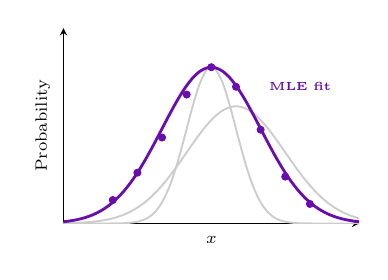
\begin{tikzpicture}[scale=0.85]
        \begin{axis}[
          width=6cm, height=4.5cm,
          axis lines=left,
          xlabel={\scriptsize $x$},
          ylabel={\scriptsize Probability},
          xtick=\empty, ytick=\empty,
          xmin=-3, xmax=3,
          ymin=0, ymax=0.5,
          tick label style={font=\tiny},
          label style={font=\tiny},
        ]
          % Data histogram hint (points)
          \addplot[only marks, mark=*, mark size=1.5pt, aiViolet]
            coordinates {(-2,0.06) (-1.5,0.13) (-1,0.22) (-0.5,0.33)
              (0,0.40) (0.5,0.35) (1,0.24) (1.5,0.12) (2,0.05)};
          % Candidate curves (light)
          \addplot[gray!40, thick, smooth, domain=-3:3, samples=40]
            {0.4*exp(-x*x/0.5)};
          \addplot[gray!40, thick, smooth, domain=-3:3, samples=40]
            {0.3*exp(-(x-0.5)*(x-0.5)/2)};
          % MLE curve (bold)
          \addplot[aiViolet, very thick, smooth, domain=-3:3, samples=40]
            {0.4*exp(-x*x/2)};
          \node[font=\tiny\bfseries, aiViolet] at (axis cs:1.8,0.35)
            {MLE fit};
        \end{axis}
      \end{tikzpicture}

      \vspace{0.2em}
      \begin{insightbox}
        LLM training is MLE at scale: find weights that maximize
        the probability of the training text. Fisher's method from 1922,
        applied to trillions of words.
      \end{insightbox}
    \end{column}
  \end{columns}

  \note{
    ``Fisher introduced the concept in 1912 and formalized it in 1922.
    He was also a pioneering statistician and controversial eugenicist ---
    we mention the math, not the politics.''

    LLM connection: LLM training is essentially maximum likelihood
    estimation: find the model parameters (weights) that maximize the
    probability of the training text.

    \verifytag{Fisher introduced concept in 1912 undergraduate paper,
    formalized in 1922 --- confirm both dates.}
  }
\end{frame}

% ----------------------------------------------------------
% Slide 32: Statistical Language Models -- Shannon's Breakthrough
% ----------------------------------------------------------
\begin{frame}{Statistical Language Models --- Shannon's Breakthrough (1948)}

  \begin{columns}[T]
    \begin{column}{0.45\textwidth}
      \begin{personbox}[Claude Shannon (1916--2001)]{aiViolet}
        \textbf{Origin:} Petoskey, Michigan, USA\\[3pt]
        Published \emph{A Mathematical Theory of Communication} (1948),
        founding information theory. Modeled English as a stochastic
        process and built \textbf{n-gram language models} decades before
        AI.
      \end{personbox}

      \vspace{0.3em}
      % Diagram: Shannon to LLM
      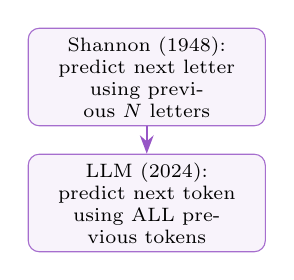
\begin{tikzpicture}[
        box/.style={draw=aiViolet!60, rounded corners, fill=aiViolet!5,
          font=\scriptsize, inner sep=3pt, text width=2.8cm, align=center},
        >=Stealth
      ]
        \node[box] (sh) at (0,0) {Shannon (1948):\\predict next letter\\using previous $N$ letters};
        \node[box] (llm) at (0,-1.6) {LLM (2024):\\predict next token\\using ALL previous tokens};
        \draw[->,thick,aiViolet!70] (sh) -- (llm);
      \end{tikzpicture}
    \end{column}

    \begin{column}{0.52\textwidth}
      % Shannon's text examples
      \begin{tcolorbox}[colback=gray!5, colframe=gray!50,
        fonttitle=\bfseries\small,
        title={Shannon's Approximations to English},
        rounded corners, boxrule=0.5pt, left=3pt, right=3pt, top=2pt, bottom=2pt]
        \scriptsize
        \textbf{0th order} (random letters):\\
        {\ttfamily XFOML RXKHRJFFJUJ}\\[2pt]
        \textbf{1st order} (letter frequencies):\\
        {\ttfamily OCRO HLI RGWR NMIE}\\[2pt]
        \textbf{2nd order} (letter pairs):\\
        {\ttfamily ON IE ANTSOUTINYS}\\[2pt]
        \textbf{Word-level bigram}:\\
        {\ttfamily THE HEAD AND IN FRONTAL ATTACK}\\[3pt]
        \textit{More context \(\Rightarrow\) more readable!}
      \end{tcolorbox}

      \vspace{0.2em}
      \begin{insightbox}
        Shannon was doing language modeling in 1948 --- 70~years
        before GPT. The same core idea, vastly more data.
      \end{insightbox}
    \end{column}
  \end{columns}

  \note{
    ``Shannon showed that language has statistical structure, and that you
    can exploit that structure to predict what comes next. That's exactly
    what every LLM does.''

    Shannon will appear AGAIN in Section 4 (Information Theory, Slide~36)
    for his entropy formula. Flag to students: ``We'll see Shannon again
    very soon --- his 1948 paper is so foundational it contributes to
    multiple sections.''
  }
\end{frame}

% ----------------------------------------------------------
% Slide 33: The Softmax Function -- From Thermodynamics to
%           Token Prediction
% ----------------------------------------------------------
\begin{frame}{The Softmax Function --- From Physics to Token Prediction}

  \begin{columns}[T]
    \begin{column}{0.46\textwidth}
      \begin{personbox}[Ludwig Boltzmann (1844--1906)]{aiViolet}
        \textbf{Origin:} Vienna, Austria\\[3pt]
        His \alert{Boltzmann distribution} (1870s) describes the
        probability of a physical system being in a state based on its
        energy: \(P \propto e^{-E/kT}\).
      \end{personbox}

      \vspace{0.3em}
      {\footnotesize
      \textbf{Lineage:}
      Boltzmann (1870s, physics) \(\to\)
      Gibbs (1900s, statistical mechanics) \(\to\)
      Luce (1959, psychology of choice) \(\to\)
      \textbf{Softmax} (ML)}

      \vspace{0.3em}
      % Conceptual recipe
      \begin{tcolorbox}[colback=aiViolet!5, colframe=aiViolet!60,
        fonttitle=\bfseries\small, title={Recipe: Softmax},
        rounded corners, boxrule=0.5pt, left=3pt, right=3pt, top=2pt, bottom=2pt]
        \footnotesize
        1. Take each raw score, raise $e$ to that power\\
        {\scriptsize\itshape (makes everything positive, magnifies differences)}\\
        2. Add up all the results\\
        3. Divide each by the total\\[2pt]
        \(\Rightarrow\) Now they are probabilities that sum to~1!
      \end{tcolorbox}
    \end{column}

    \begin{column}{0.51\textwidth}
      % Softmax pipeline
      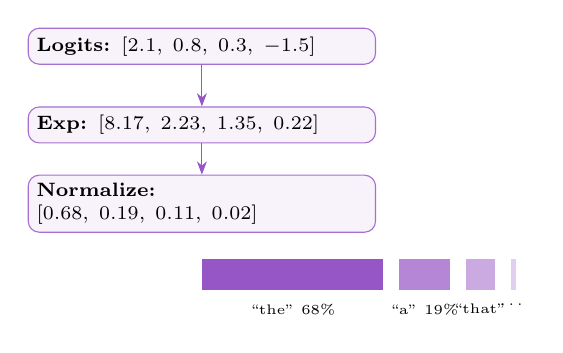
\begin{tikzpicture}[
        softstep/.style={draw=aiViolet!60, rounded corners, fill=aiViolet!5,
          font=\scriptsize, inner sep=3pt, text width=4.2cm, align=left},
        >=Stealth
      ]
        \node[softstep] (s1) at (0, 3.0)
          {\textbf{Logits:} $[2.1,\; 0.8,\; 0.3,\; {-}1.5]$};
        \node[softstep] (s2) at (0, 2.0)
          {\textbf{Exp:} $[8.17,\; 2.23,\; 1.35,\; 0.22]$};
        \node[softstep] (s3) at (0, 1.0)
          {\textbf{Normalize:} $[0.68,\; 0.19,\; 0.11,\; 0.02]$};
        \draw[->,aiViolet!70] (s1.south) -- (s2.north);
        \draw[->,aiViolet!70] (s2.south) -- (s3.north);

        % Bar chart
        \fill[aiViolet!70] (0, -0.1) rectangle (2.3, 0.3);
        \fill[aiViolet!50] (2.5, -0.1) rectangle (3.15, 0.3);
        \fill[aiViolet!35] (3.35, -0.1) rectangle (3.72, 0.3);
        \fill[aiViolet!20] (3.92, -0.1) rectangle (3.99, 0.3);
        \node[font=\tiny,below] at (1.15, -0.15) {``the'' 68\%};
        \node[font=\tiny,below] at (2.82, -0.15) {``a'' 19\%};
        \node[font=\tiny,below] at (3.53, -0.15) {``that''};
        \node[font=\tiny,below] at (3.95, -0.15) {\ldots};
      \end{tikzpicture}

      \vspace{0.3em}
      % Formal inset
      \begin{tcolorbox}[colback=gray!5, colframe=gray!40,
        fonttitle=\bfseries\small, title={Formal},
        rounded corners, boxrule=0.5pt, left=3pt, right=3pt, top=1pt, bottom=1pt]
        \footnotesize
        $\displaystyle \mathrm{softmax}(z_i) = \frac{e^{z_i}}{\sum_j e^{z_j}}$
        \hfill {\scriptsize $\sum$ = ``add up for all $j$''}
      \end{tcolorbox}
    \end{column}
  \end{columns}

  \note{
    ``Boltzmann invented this formula to describe how gas molecules
    distribute among energy states. 150 years later, the exact same
    formula tells an LLM which word to say next.''

    INTERACTIVE MOMENT: Quick poll --- ``What word comes next:
    `The cat sat on the \rule{1cm}{0.15mm}'?'' Collect student answers,
    then show the AI's softmax distribution for the same prompt.

    \verifytag{Boltzmann distribution typically dated to 1870s; ``1868''
    may refer to early papers. R.~Duncan Luce's 1959 book
    \emph{Individual Choice Behavior} --- confirm.}
  }
\end{frame}

% ----------------------------------------------------------
% Slide 34: Convergence Diagram Update -- Probability
% ----------------------------------------------------------
\begin{frame}{Building the Transformer --- Probability \& Statistics}

  \begin{columns}[T]
    \begin{column}{0.45\textwidth}
      % Convergence diagram placeholder
      \visualplaceholder[5cm]{Convergence diagram: Sections 1--2 lit
        (Linear Algebra in blue, Calculus in green). Section~3
        ``Probability \& Statistics'' now lights up in orange/violet.
        Label: ``Softmax = next-token prediction.''}
    \end{column}

    \begin{column}{0.52\textwidth}
      \begin{tcolorbox}[colback=aiViolet!5, colframe=aiViolet,
        fonttitle=\bfseries, title={Section 3 Summary},
        rounded corners, boxrule=1pt, left=4pt, right=4pt, top=3pt, bottom=3pt]
        \footnotesize
        \begin{tabular}{@{}ll@{}}
          \toprule
          \textbf{Who / When} & \textbf{Contribution}\\
          \midrule
          Pascal / Fermat (1654) & Birth of probability\\
          Bernoulli (1713) & Law of large numbers\\
          Bayes (1763) / Laplace & Updating beliefs from evidence\\
          Kolmogorov (1933) & Rigorous axioms\\
          Fisher (1922) & Maximum likelihood estimation\\
          Shannon (1948) & Language as a statistical process\\
          Boltzmann (1870s) & \(\to\) Luce (1959) \(\to\) Softmax\\
          \bottomrule
        \end{tabular}
      \end{tcolorbox}

      \vspace{0.3em}
      \begin{insightbox}
        Every time an LLM generates a word, it computes a softmax
        probability distribution. The math started with a gambling
        question in 1654.
      \end{insightbox}
    \end{column}
  \end{columns}

  \note{
    Connection arrow: ``Every time an LLM generates a word, it computes
    a softmax probability distribution. The math started with a gambling
    question in 1654.''

    Transition: ``The network predicts probabilities. But how do we
    measure whether those probabilities are GOOD? For that, we need
    information theory.''
  }
\end{frame}


% ************************************************************
% SECTION 4: INFORMATION THEORY (Slides 35-41)
% "Measuring Meaning"
% Section color: aiViolet
% ************************************************************
\section{Information Theory}

% ----------------------------------------------------------
% Slide 35: Section Divider
% ----------------------------------------------------------
{
\setbeamercolor{background canvas}{bg=aiViolet}
\begin{frame}[plain]
  \centering
  \vspace{2cm}
  \textcolor{white}{\Huge\bfseries Information Theory}\\[0.5em]
  \textcolor{white}{\Huge\bfseries Measuring Meaning}\\[1em]
  \textcolor{white!80}{\large 1865--1948}\\[1.5em]
  \textcolor{white!60}{\normalsize Clausius \(\cdot\) Boltzmann \(\cdot\) Shannon \(\cdot\) Kullback \(\cdot\) Zipf}

  \note{
    Transition: ``The network predicts probabilities. But how do we
    measure whether those probabilities are GOOD? For that, we need
    information theory.''

    Tagline: How surprised should you be by the next word? Information
    theory measures that.

    This section covers \(\sim\)8 minutes.
  }
\end{frame}
}

% ----------------------------------------------------------
% Slide 36: Entropy -- From Steam Engines to Bits
% ----------------------------------------------------------
\begin{frame}{Entropy --- Invented Three Times}

  \begin{columns}[T]
    \begin{column}{0.32\textwidth}
      % Column 1: Clausius
      \begin{tcolorbox}[colback=aiViolet!5, colframe=aiViolet!60,
        fonttitle=\bfseries\scriptsize, title={Clausius (1865)},
        rounded corners, boxrule=0.5pt, left=2pt, right=2pt, top=2pt, bottom=2pt]
        \scriptsize
        \visualplaceholder[3cm]{Steam engine diagram}
        Entropy as ``energy unavailable for work.''
        Named from Greek \emph{entropia} (transformation).
      \end{tcolorbox}
    \end{column}

    \begin{column}{0.32\textwidth}
      % Column 2: Boltzmann
      \begin{tcolorbox}[colback=aiViolet!5, colframe=aiViolet!60,
        fonttitle=\bfseries\scriptsize, title={Boltzmann (1870s)},
        rounded corners, boxrule=0.5pt, left=2pt, right=2pt, top=2pt, bottom=2pt]
        \scriptsize
        \visualplaceholder[3cm]{Gas molecules in a box; Boltzmann's
          tombstone with $S = k \log W$}
        Entropy as ``number of arrangements.''
        \[S = k \log W\]
      \end{tcolorbox}
    \end{column}

    \begin{column}{0.32\textwidth}
      % Column 3: Shannon
      \begin{tcolorbox}[colback=aiViolet!5, colframe=aiViolet!60,
        fonttitle=\bfseries\scriptsize, title={Shannon (1948)},
        rounded corners, boxrule=0.5pt, left=2pt, right=2pt, top=2pt, bottom=2pt]
        \scriptsize
        \visualplaceholder[3cm]{Fair coin vs loaded coin; entropy
          formula diagram}
        Entropy as ``average surprise.''
        \[H = -\!\sum_i p_i \log p_i\]
        {\tiny $\sum$ = ``add up for every outcome $i$''}
      \end{tcolorbox}
    \end{column}
  \end{columns}

  \vspace{0.3em}
  {\small\centering\itshape The same formula. Three completely different domains.\par}

  \note{
    CROSS-REFERENCE: Shannon appears again! We saw him in Section~3
    (statistical language models, Slide~32). His 1948 paper is so
    foundational that it contributes to BOTH the probability and
    information theory sections. He modeled language statistically AND
    created the measure for how good that model is.

    Conceptual recipe for Shannon's formula: ``For each possible outcome,
    multiply its probability by the `surprise' (the logarithm of how
    unexpected it is). Add them all up. The result is the average
    surprise.''

    Anecdote: ``Shannon supposedly asked von Neumann what to call his new
    quantity. Von Neumann said: `Call it entropy. Nobody knows what
    entropy really is, so in a debate you will always have the
    advantage.'\,'' (May be apocryphal.)

    \verifytag{Clausius coined ``entropy'' in 1865 but the concept appears
    in his earlier 1850s work. Shannon--von Neumann anecdote is widely
    attributed but may be apocryphal.}
  }
\end{frame}

% ----------------------------------------------------------
% Slide 37: Cross-Entropy -- The Loss Function of LLMs
% ----------------------------------------------------------
\begin{frame}{Cross-Entropy --- THE Loss Function of LLMs}

  \begin{columns}[T]
    \begin{column}{0.46\textwidth}
      % Conceptual recipe
      \begin{tcolorbox}[colback=aiViolet!5, colframe=aiViolet!60,
        fonttitle=\bfseries\small, title={Recipe: Cross-Entropy Loss},
        rounded corners, boxrule=0.5pt, left=3pt, right=3pt, top=3pt, bottom=3pt]
        \footnotesize
        1. The true answer is one specific word.\\
        2. Look at the probability your model gave that word.\\
        3. Take the logarithm.\\
        4. Negate it.\\[3pt]
        High confidence in right answer \(\Rightarrow\) low loss.\\
        Low confidence in right answer \(\Rightarrow\) high loss.
      \end{tcolorbox}

      \vspace{0.3em}
      % Formal inset
      \begin{tcolorbox}[colback=gray!5, colframe=gray!40,
        fonttitle=\bfseries\small, title={Formal},
        rounded corners, boxrule=0.5pt, left=3pt, right=3pt, top=1pt, bottom=1pt]
        \footnotesize
        \[\text{Loss} = -\log\bigl(p_{\text{model}}(\text{correct token})\bigr)\]
        {\scriptsize Full form uses $\sum$ over all tokens, but since
        only one is correct, it simplifies to this.}
      \end{tcolorbox}
    \end{column}

    \begin{column}{0.51\textwidth}
      % Concrete example
      {\footnotesize ``The cat sat on the \rule{0.8cm}{0.4pt}''}

      \vspace{0.3em}
      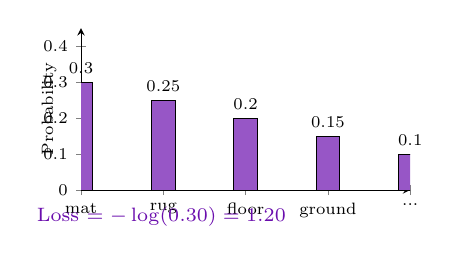
\begin{tikzpicture}[scale=0.85]
        \begin{axis}[
          width=6.5cm, height=4cm,
          ybar,
          bar width=10pt,
          ylabel={\scriptsize Probability},
          ylabel style={at={(axis description cs:-0.05,0.5)}},
          symbolic x coords={mat, rug, floor, ground, ...},
          xtick=data,
          tick label style={font=\scriptsize},
          label style={font=\scriptsize},
          ymin=0, ymax=0.45,
          ytick={0,0.1,0.2,0.3,0.4},
          axis lines=left,
          nodes near coords={\scriptsize\pgfmathprintnumber\pgfplotspointmeta},
          every node near coord/.append style={font=\tiny},
        ]
          \addplot[fill=aiViolet!70] coordinates
            {(mat,0.30) (rug,0.25) (floor,0.20) (ground,0.15) (...,0.10)};
        \end{axis}
        \node[font=\scriptsize,aiViolet] at (1.2,-0.4)
          {Loss $= -\log(0.30) = 1.20$};
      \end{tikzpicture}

      \vspace{0.1em}
      {\scriptsize If model improves to 80\% for ``mat'':
       loss $= -\log(0.80) = 0.22$}

      \vspace{0.2em}
      \begin{insightbox}
        Training an LLM = minimizing cross-entropy = making the model
        more confident about the RIGHT next word.
      \end{insightbox}
    \end{column}
  \end{columns}

  \note{
    ``Every time an LLM gets a training example, it predicts the next
    token, checks how wrong it was using cross-entropy, then uses
    backpropagation (Section~2!) to improve. Cross-entropy is the bridge
    between information theory and gradient descent.''

    Bridge to earlier sections: Softmax (Section~3) produces the
    probabilities. Cross-entropy measures how good they are.
    Backpropagation (Section~2) improves them.
  }
\end{frame}

% ----------------------------------------------------------
% Slide 38: Surprisal and Perplexity
% ----------------------------------------------------------
\begin{frame}{Surprisal and Perplexity --- How We Evaluate LLMs}

  \begin{columns}[T]
    \begin{column}{0.47\textwidth}
      \begin{tcolorbox}[colback=aiViolet!5, colframe=aiViolet!60,
        fonttitle=\bfseries\small, title={Surprisal},
        rounded corners, boxrule=0.5pt, left=3pt, right=3pt, top=3pt, bottom=3pt]
        \footnotesize
        $\text{Surprisal} = -\log\bigl(p(\text{word})\bigr)$\\[3pt]
        High probability \(\Rightarrow\) low surprisal\\
        Low probability \(\Rightarrow\) high surprisal
      \end{tcolorbox}

      \vspace{0.3em}
      \begin{tcolorbox}[colback=aiViolet!5, colframe=aiViolet!60,
        fonttitle=\bfseries\small, title={Perplexity},
        rounded corners, boxrule=0.5pt, left=3pt, right=3pt, top=3pt, bottom=3pt]
        \footnotesize
        Average surprisal, exponentiated.\\[3pt]
        Lower perplexity = better model.\\[3pt]
        {\scriptsize ``GPT-4 has lower perplexity than GPT-3'' means
        it's less surprised by real text.}
      \end{tcolorbox}

      \vspace{0.3em}
      \begin{insightbox}
        A good language model is rarely surprised by real text.
        Shannon would have understood this immediately.
      \end{insightbox}
    \end{column}

    \begin{column}{0.5\textwidth}
      % Surprisal example
      {\footnotesize ``The cat sat on the \rule{0.8cm}{0.4pt}''}

      \vspace{0.4em}
      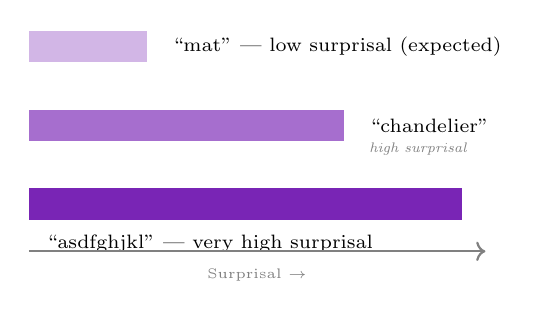
\begin{tikzpicture}[
        bar/.style={draw=none, rounded corners=1pt},
        lbl/.style={font=\scriptsize, anchor=west},
      ]
        % mat -- low surprisal
        \fill[aiViolet!30] (0, 2.4) rectangle (1.5, 2.8);
        \node[lbl] at (1.7, 2.6) {``mat'' --- low surprisal (expected)};

        % chandelier -- high surprisal
        \fill[aiViolet!60] (0, 1.4) rectangle (4.0, 1.8);
        \node[lbl] at (4.2, 1.6) {``chandelier''};
        \node[font=\tiny\itshape,gray,anchor=west] at (4.2,1.3) {high surprisal};

        % asdfghjkl -- very high
        \fill[aiViolet!90] (0, 0.4) rectangle (5.5, 0.8);
        \node[lbl] at (0.1, 0.1) {``asdfghjkl'' --- very high surprisal};

        % Arrow label
        \draw[->,thick,gray] (0,0.0) -- (5.8,0.0);
        \node[font=\tiny,gray,anchor=north] at (2.9,-0.1) {Surprisal \(\to\)};
      \end{tikzpicture}
    \end{column}
  \end{columns}

  \note{
    ``When researchers say GPT-4 has `lower perplexity' than GPT-3, they
    mean it's less surprised by real text --- it predicts better.
    Shannon would have understood this immediately.''

    Perplexity is the standard evaluation metric for language models. It
    connects directly to Shannon's information-theoretic framework.
  }
\end{frame}

% ----------------------------------------------------------
% Slide 39: KL Divergence [EXTENDED]
% ----------------------------------------------------------
\begin{frame}{KL Divergence --- Measuring the Gap Between Distributions}

  \begin{columns}[T]
    \begin{column}{0.47\textwidth}
      {\footnotesize
      \textbf{Solomon Kullback} (1907--1994) \&
      \textbf{Richard Leibler} (1914--2003), USA.\\
      Published KL divergence in 1951.}

      \vspace{0.3em}
      % Conceptual recipe
      \begin{tcolorbox}[colback=aiViolet!5, colframe=aiViolet!60,
        fonttitle=\bfseries\small, title={Recipe: KL Divergence},
        rounded corners, boxrule=0.5pt, left=3pt, right=3pt, top=2pt, bottom=2pt]
        \footnotesize
        For each possible outcome, ask:\\
        ``How much more surprising is this under model $Q$ compared to
        truth $P$?''\\[3pt]
        Average over all outcomes.\\[3pt]
        If $Q$ matches $P$ perfectly $\Rightarrow$ KL $= 0$.
      \end{tcolorbox}

      \vspace{0.3em}
      \begin{insightbox}
        In RLHF (the technique that makes ChatGPT helpful), KL divergence
        prevents the model from changing too much during fine-tuning.
      \end{insightbox}

      \vspace{0.2em}
      {\footnotesize\textcolor{gray}{[EXTENDED] --- can be cut without
      losing the narrative}}
    \end{column}

    \begin{column}{0.5\textwidth}
      % Two overlapping distributions
      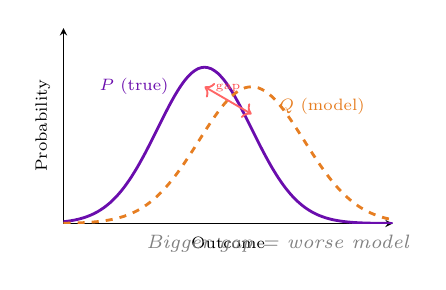
\begin{tikzpicture}[scale=0.85]
        \begin{axis}[
          width=6.5cm, height=4.5cm,
          axis lines=left,
          xlabel={\scriptsize Outcome},
          ylabel={\scriptsize Probability},
          xtick=\empty, ytick=\empty,
          xmin=-3, xmax=4,
          ymin=0, ymax=0.5,
          tick label style={font=\tiny},
          label style={font=\tiny},
        ]
          % P (true)
          \addplot[aiViolet, very thick, smooth, domain=-3:4, samples=50]
            {0.4*exp(-x*x/2)};
          % Q (model)
          \addplot[accentOrange, very thick, smooth, dashed, domain=-3:4, samples=50]
            {0.35*exp(-(x-1)*(x-1)/2.5)};
          % Gap annotation
          \draw[<->, thick, red!60] (axis cs:0,0.35) -- (axis cs:1,0.28)
            node[midway, above, font=\tiny, text=red!70] {gap};
          \node[font=\scriptsize, aiViolet] at (axis cs:-1.5,0.35) {$P$ (true)};
          \node[font=\scriptsize, accentOrange] at (axis cs:2.5,0.3) {$Q$ (model)};
        \end{axis}
        \node[font=\scriptsize\itshape,gray] at (3.2,-0.3)
          {Bigger gap = worse model};
      \end{tikzpicture}

      \vspace{0.3em}
      % Formal
      \begin{tcolorbox}[colback=gray!5, colframe=gray!40,
        fonttitle=\bfseries\small, title={Formal},
        rounded corners, boxrule=0.5pt, left=3pt, right=3pt, top=1pt, bottom=1pt]
        \footnotesize
        $\displaystyle D_{\text{KL}}(P \| Q) = \sum_i P(i)\,\log\frac{P(i)}{Q(i)}$
      \end{tcolorbox}
    \end{column}
  \end{columns}

  \note{
    This slide is marked [EXTENDED] and can be cut if time is short.

    ``In RLHF (Reinforcement Learning from Human Feedback), KL divergence
    is used to prevent the model from diverging too far from its base
    behavior during fine-tuning.''

    \verifytag{Kullback--Leibler 1951 paper ``On Information and
    Sufficiency'' --- confirm title and year.}
  }
\end{frame}

% ----------------------------------------------------------
% Slide 40: Tokenization -- Carving Language into Pieces
% ----------------------------------------------------------
\begin{frame}{Tokenization --- Carving Language into Pieces}

  \begin{columns}[T]
    \begin{column}{0.46\textwidth}
      {\footnotesize
      \textbf{George Kingsley Zipf} (1902--1950, USA).\\
      \alert{Zipf's law} (1935/1949): word frequency is inversely
      proportional to its rank. ``The'' is \#1, ``of'' is \#2, \ldots}

      \vspace{0.3em}
      {\footnotesize
      \textbf{Rico Sennrich}, \textbf{Barry Haddow},
      \textbf{Alexandra Birch} (Edinburgh, 2016).\\
      Adapted \alert{Byte Pair Encoding} (BPE) for neural machine
      translation. BPE is the tokenization method used by GPT and most
      modern LLMs.}

      \vspace{0.3em}
      \begin{insightbox}
        The AI doesn't see words --- it sees tokens. BPE gives short
        tokens to common patterns (Zipf's law!) and splits rare words
        into pieces.
      \end{insightbox}
    \end{column}

    \begin{column}{0.51\textwidth}
      % Tokenization example
      \begin{tcolorbox}[colback=aiViolet!5, colframe=aiViolet!60,
        fonttitle=\bfseries\small, title={BPE Tokenization Example},
        rounded corners, boxrule=0.5pt, left=3pt, right=3pt, top=3pt, bottom=3pt]
        \footnotesize
        \textbf{Input:}\\
        {\ttfamily The mathematician calculated the eigenvalue}\\[4pt]
        \textbf{Tokens:}\\
        \colorbox{aiViolet!15}{\ttfamily The}\;
        \colorbox{aiViolet!25}{\ttfamily\, mathematic}\,%
        \colorbox{aiViolet!35}{\ttfamily ian}\;
        \colorbox{aiViolet!15}{\ttfamily\, calculated}\;
        \colorbox{aiViolet!15}{\ttfamily\, the}\;
        \colorbox{aiViolet!25}{\ttfamily\, eigen}\,%
        \colorbox{aiViolet!35}{\ttfamily value}\\[4pt]
        {\scriptsize Common words \(\to\) single token\\
        Rare words \(\to\) split into pieces}
      \end{tcolorbox}

      \vspace{0.3em}
      % Zipf's law sketch
      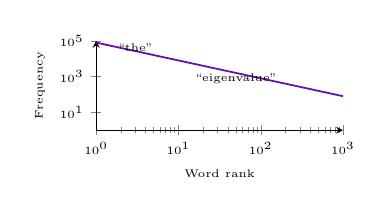
\begin{tikzpicture}[scale=0.8]
        \begin{axis}[
          width=5.5cm, height=3cm,
          axis lines=left,
          xlabel={\tiny Word rank},
          ylabel={\tiny Frequency},
          xtick={1,10,100,1000},
          xmode=log,
          ymode=log,
          ymin=1, ymax=100000,
          tick label style={font=\tiny},
          label style={font=\tiny},
        ]
          \addplot[aiViolet, thick, domain=1:1000, samples=30] {80000/x};
          \node[font=\tiny] at (axis cs:3,40000) {``the''};
          \node[font=\tiny] at (axis cs:50,800) {``eigenvalue''};
        \end{axis}
      \end{tikzpicture}
    \end{column}
  \end{columns}

  \note{
    ``Common words like `the' get one token. Uncommon words like
    `eigenvalue' get split into `eigen' + `value.' This encoding scheme
    is deeply connected to information theory: give short codes to
    frequent patterns.''

    Historical lineage: Philip Gage published BPE as a compression
    algorithm in 1994. Sennrich et al.\ adapted it for NLP in 2016.

    \verifytag{Zipf's law appears in his 1935 book and more fully in his
    1949 book. Sennrich et al.\ 2016 ACL paper --- confirm venue.}
  }
\end{frame}

% ----------------------------------------------------------
% Slide 41: Convergence Diagram Update -- Information Theory
% ----------------------------------------------------------
\begin{frame}{Building the Transformer --- Information Theory}

  \begin{columns}[T]
    \begin{column}{0.45\textwidth}
      % Convergence diagram placeholder
      \visualplaceholder[5cm]{Convergence diagram: Sections 1--3 lit
        (Linear Algebra, Calculus, Probability). Section~4
        ``Information Theory'' now lights up in red.
        Label: ``Cross-entropy = the loss function.''}
    \end{column}

    \begin{column}{0.52\textwidth}
      \begin{tcolorbox}[colback=aiViolet!5, colframe=aiViolet,
        fonttitle=\bfseries, title={Section 4 Summary},
        rounded corners, boxrule=1pt, left=4pt, right=4pt, top=3pt, bottom=3pt]
        \footnotesize
        \begin{tabular}{@{}ll@{}}
          \toprule
          \textbf{Who / When} & \textbf{Contribution}\\
          \midrule
          Clausius (1865) & Thermodynamic entropy\\
          Boltzmann (1870s) & Statistical entropy, $S = k\log W$\\
          Shannon (1948) & Information entropy, the ``bit''\\
          Kullback--Leibler (1951) & Divergence between distributions\\
          Zipf (1935/1949) & Word frequency laws\\
          Sennrich et al.\ (2016) & BPE tokenization\\
          \bottomrule
        \end{tabular}
      \end{tcolorbox}

      \vspace{0.3em}
      \begin{insightbox}
        LLMs are trained by minimizing cross-entropy loss.
        Shannon's 1948 formula is literally the objective function.
      \end{insightbox}
    \end{column}
  \end{columns}

  \note{
    Connection arrow: ``LLMs are trained by minimizing cross-entropy
    loss. Shannon's 1948 formula is literally the objective function.''

    Transition: ``We have the math for learning and the math for
    measuring. But we need something to run it on. Enter: logic and
    computation.''
  }
\end{frame}


% ************************************************************
% SECTION 5: LOGIC & COMPUTATION (Slides 42-48)
% "The Substrate"
% Section color: aiViolet
%
% NARRATIVE TENSION: Logicians dreamed of mechanical reasoning.
% They proved it was impossible. Then neural networks did it
% anyway.
% ************************************************************
\section{Logic \& Computation}

% ----------------------------------------------------------
% Slide 42: Section Divider
% ----------------------------------------------------------
{
\setbeamercolor{background canvas}{bg=aiViolet}
\begin{frame}[plain]
  \centering
  \vspace{2cm}
  \textcolor{white}{\Huge\bfseries Logic \& Computation}\\[0.5em]
  \textcolor{white}{\Huge\bfseries The Substrate}\\[1em]
  \textcolor{white!80}{\large 1854--1970s}\\[1.5em]
  \textcolor{white!60}{\normalsize Boole \(\cdot\) Frege \(\cdot\) G\"odel \(\cdot\) Turing \(\cdot\) von Neumann}\\[1em]
  \textcolor{white!70}{\itshape\normalsize ``Logicians dreamed of mechanical thought.\\
    They proved it was impossible.\\
    Then neural networks did it anyway.''}

  \note{
    Transition: ``We have the math for learning and the math for
    measuring. But we need something to run it on.''

    This section is structured around a paradox: logicians tried to
    reduce all reasoning to mechanical rules, Turing and G\"odel proved
    that's impossible, and yet neural networks learned to do things
    formal logic cannot: translate, write poetry, reason by analogy.

    The machines that logic built transcended the limitations that logic
    discovered.

    This section covers \(\sim\)8 minutes.
  }
\end{frame}
}

% ----------------------------------------------------------
% Slide 43: Boolean Algebra -- The Language of Computers
% ----------------------------------------------------------
\begin{frame}{Boolean Algebra --- The Language of Computers (1854)}

  \begin{columns}[T]
    \begin{column}{0.45\textwidth}
      \begin{personbox}[George Boole (1815--1864)]{aiViolet}
        \textbf{Origin:} Lincoln, England; worked at Queen's College
        Cork, Ireland\\[3pt]
        Published \emph{An Investigation of the Laws of Thought} (1854).
        Self-taught mathematician who showed that \textbf{logical
        reasoning} could be expressed as \textbf{algebra}: variables
        take values 0 (false) or 1 (true).
      \end{personbox}

      \vspace{0.3em}
      \begin{insightbox}
        Boole was a self-taught son of a shoemaker who became a
        university professor. His algebra is now the foundation of every
        digital device on Earth.
      \end{insightbox}
    \end{column}

    \begin{column}{0.52\textwidth}
      % Boolean logic gates
      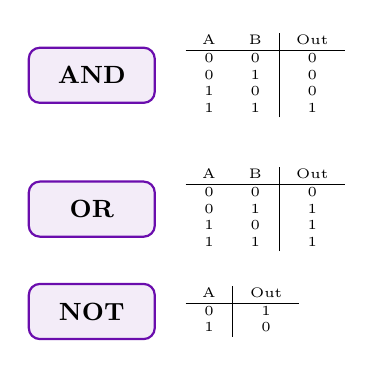
\begin{tikzpicture}[
        gate/.style={draw=aiViolet, thick, rounded corners, fill=aiViolet!8,
          minimum width=1.6cm, minimum height=0.7cm, font=\small\bfseries,
          align=center},
        tbl/.style={font=\tiny, inner sep=2pt},
        >=Stealth
      ]
        % AND gate
        \node[gate] (and) at (0, 2.5) {AND};
        \node[tbl,right=0.3cm of and] {%
          \begin{tabular}{cc|c}
            A & B & Out\\ \hline
            0 & 0 & 0\\
            0 & 1 & 0\\
            1 & 0 & 0\\
            1 & 1 & 1
          \end{tabular}
        };

        % OR gate
        \node[gate] (or) at (0, 0.8) {OR};
        \node[tbl,right=0.3cm of or] {%
          \begin{tabular}{cc|c}
            A & B & Out\\ \hline
            0 & 0 & 0\\
            0 & 1 & 1\\
            1 & 0 & 1\\
            1 & 1 & 1
          \end{tabular}
        };

        % NOT gate
        \node[gate] (not) at (0, -0.5) {NOT};
        \node[tbl,right=0.3cm of not] {%
          \begin{tabular}{c|c}
            A & Out\\ \hline
            0 & 1\\
            1 & 0
          \end{tabular}
        };
      \end{tikzpicture}

      \vspace{0.3em}
      {\small\centering Every GPU in every AI data center is made of
      \emph{billions} of these gates.\par}
    \end{column}
  \end{columns}

  \note{
    ``Boolean algebra reduced logical reasoning to symbols and rules.
    Every digital computer --- from your phone to a data center full of
    GPUs --- is built from AND, OR, and NOT gates. Billions of them.''

    Boole's work was abstract and philosophical. He had no idea it would
    become the foundation of hardware.
  }
\end{frame}

% ----------------------------------------------------------
% Slide 44: The Dream and Its Limits -- Frege to Godel to Turing
% ----------------------------------------------------------
\begin{frame}{The Dream and Its Limits --- From Frege to Turing}

  {\small After Boole, logicians dreamed of reducing ALL reasoning to
  mechanical symbol manipulation. They almost succeeded --- and then
  proved it was \textbf{impossible}.}

  \vspace{0.3em}
  % Timeline
  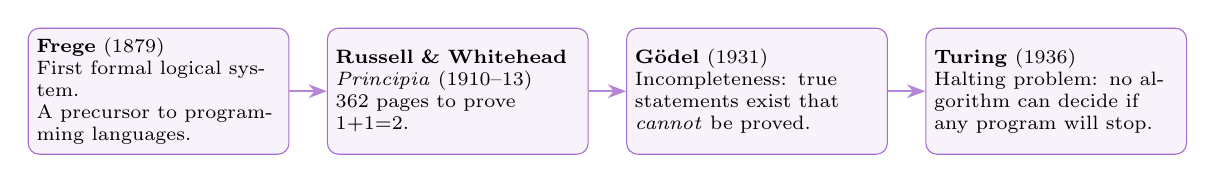
\begin{tikzpicture}[
    person/.style={draw=aiViolet!60, rounded corners, fill=aiViolet!5,
      font=\scriptsize, inner sep=3pt, text width=3.1cm, align=left,
      minimum height=1.6cm},
    arr/.style={-Stealth, thick, aiViolet!50},
  ]
    \node[person] (frege) at (0, 0) {%
      \textbf{Frege} (1879)\\
      First formal logical system.\\
      A precursor to programming languages.};
    \node[person] (rw) at (3.8, 0) {%
      \textbf{Russell \& Whitehead}\\
      \emph{Principia} (1910--13)\\
      362 pages to prove $1{+}1{=}2$.};
    \node[person] (godel) at (7.6, 0) {%
      \textbf{G\"odel} (1931)\\
      \alert{Incompleteness:} true statements exist that \emph{cannot}
      be proved.};
    \node[person] (turing) at (11.4, 0) {%
      \textbf{Turing} (1936)\\
      \alert{Halting problem:} no algorithm can decide if any program
      will stop.};

    \draw[arr] (frege.east) -- (rw.west);
    \draw[arr] (rw.east) -- (godel.west);
    \draw[arr] (godel.east) -- (turing.west);
  \end{tikzpicture}

  \vspace{0.3em}
  \begin{insightbox}
    The irony: neural networks, built from Boole's logic gates, learned
    to translate, reason, and create --- not by following rules, but by
    learning patterns from data. The machines that logic built went
    beyond what logic can do.
  \end{insightbox}

  \note{
    Key persons (brief):
    \begin{itemize}\setlength\itemsep{1pt}
      \item \textbf{Gottlob Frege} (1848--1925, Wismar, Germany).
        Created the first formal logic powerful enough to express math
        (\emph{Begriffsschrift}, 1879).
      \item \textbf{Bertrand Russell} (1872--1970) \&
        \textbf{Alfred North Whitehead} (1861--1947).
        \emph{Principia Mathematica} (1910--1913): derive ALL math from
        logical axioms.
      \item \textbf{Kurt G\"odel} (1906--1978, Brno / Princeton).
        Incompleteness theorems (1931).
      \item \textbf{Alan Turing} (1912--1954, London). ``On Computable
        Numbers'' (1936): the Turing machine and the halting problem.
    \end{itemize}

    ``They tried to reduce all reasoning to logic. G\"odel proved some
    truths escape any formal system. Turing proved some questions can't
    be answered by any algorithm. And yet --- neural networks, built from
    Boole's logic gates, learned to translate, reason, and create.''

    \verifytag{Page number 362 for 1+1=2 in Principia is commonly cited
    but may be approximate.}
  }
\end{frame}

% ----------------------------------------------------------
% Slide 45: Von Neumann Architecture [EXTENDED]
% ----------------------------------------------------------
\begin{frame}{Von Neumann Architecture --- The Hardware Blueprint (1945)}

  \begin{columns}[T]
    \begin{column}{0.45\textwidth}
      \begin{personbox}[John von Neumann (1903--1957)]{aiViolet}
        \textbf{Born:} Neumann J\'anos Lajos\\
        \textbf{Origin:} Budapest, Hungary; worked at Princeton, USA\\[3pt]
        Published \emph{First Draft of a Report on the EDVAC} (1945),
        describing the \alert{stored-program architecture}: instructions
        and data share the same memory.
      \end{personbox}

      \vspace{0.3em}
      {\footnotesize\textcolor{gray}{[EXTENDED] --- can be cut;
      summarize verbally}}

      \vspace{0.2em}
      {\small\itshape LLM inference runs on this architecture. But
      training requires massively parallel hardware. Enter the GPU.}
    \end{column}

    \begin{column}{0.52\textwidth}
      % Von Neumann architecture diagram
      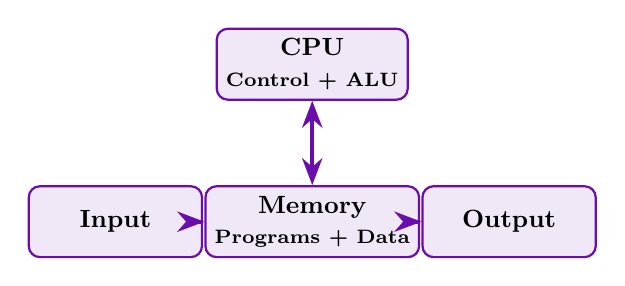
\begin{tikzpicture}[
        comp/.style={draw=aiViolet, thick, rounded corners=4pt,
          fill=aiViolet!10, minimum width=2.2cm, minimum height=0.9cm,
          font=\small\bfseries, align=center},
        bus/.style={draw=aiViolet, thick, -Stealth, line width=1.5pt},
        dbus/.style={draw=aiViolet, thick, Stealth-Stealth, line width=1.5pt},
      ]
        \node[comp] (cpu) at (0, 2) {CPU\\{\scriptsize Control + ALU}};
        \node[comp] (mem) at (0, 0) {Memory\\{\scriptsize Programs + Data}};
        \node[comp] (inp) at (-2.5, 0) {Input};
        \node[comp] (out) at (2.5, 0) {Output};

        \draw[dbus] (cpu) -- (mem);
        \draw[bus] (inp) -- (mem);
        \draw[bus] (mem) -- (out);
      \end{tikzpicture}

      \vspace{0.4em}
      {\small\centering This basic design has powered nearly every
      computer for 80~years.\par}
    \end{column}
  \end{columns}

  \note{
    ``The stored-program concept: keep both the program and its data in
    the same memory. Nearly every computer follows this design.''

    Note: the 1945 draft was controversial --- it was circulated under
    von Neumann's name alone, but was based on collaborative work by
    Eckert and Mauchly. We present the architecture concept, not the
    priority dispute.

    \verifytag{First Draft of a Report on the EDVAC, 1945 --- confirm
    attribution context.}
  }
\end{frame}

% ----------------------------------------------------------
% Slide 46: Floating Point Arithmetic
% ----------------------------------------------------------
\begin{frame}{Floating Point --- How Computers Handle Real Numbers}

  \begin{columns}[T]
    \begin{column}{0.48\textwidth}
      {\footnotesize
      \textbf{Konrad Zuse} (1910--1995, Berlin, Germany).\\
      Built the \alert{Z3} (1941), the first programmable computer using
      floating-point arithmetic.}

      \vspace{0.3em}
      % Floating-point layout
      \begin{tcolorbox}[colback=aiViolet!5, colframe=aiViolet!60,
        fonttitle=\bfseries\small, title={How 3.14159 is stored},
        rounded corners, boxrule=0.5pt, left=3pt, right=3pt, top=3pt, bottom=3pt]
        \footnotesize
        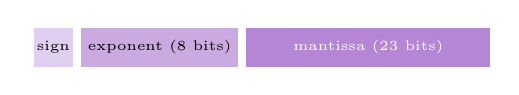
\begin{tikzpicture}
          \fill[aiViolet!20] (0,0) rectangle (0.5,0.5);
          \node[font=\tiny] at (0.25,0.25) {sign};
          \fill[aiViolet!35] (0.6,0) rectangle (2.6,0.5);
          \node[font=\tiny] at (1.6,0.25) {exponent (8 bits)};
          \fill[aiViolet!50] (2.7,0) rectangle (5.8,0.5);
          \node[font=\tiny,white] at (4.25,0.25) {mantissa (23 bits)};
        \end{tikzpicture}

        \vspace{2pt}
        {\scriptsize IEEE 754 standard (1985)}
      \end{tcolorbox}

      \vspace{0.3em}
      \begin{insightbox}
        Every weight in an LLM is a floating-point number. Large models
        have hundreds of billions of them.
      \end{insightbox}
    \end{column}

    \begin{column}{0.49\textwidth}
      % Precision comparison
      \begin{tcolorbox}[colback=gray!5, colframe=gray!50,
        fonttitle=\bfseries\small,
        title={Precision vs.\ Speed Trade-off},
        rounded corners, boxrule=0.5pt, left=3pt, right=3pt, top=3pt, bottom=3pt]
        \footnotesize
        \begin{tabular}{@{}lcc@{}}
          \toprule
          \textbf{Format} & \textbf{Bits} & \textbf{Use}\\
          \midrule
          FP32 & 32 & Traditional training\\
          FP16 / BF16 & 16 & Modern LLM training\\
          INT8 & 8 & Fast inference\\
          INT4 & 4 & Aggressive compression\\
          \bottomrule
        \end{tabular}

        \vspace{4pt}
        {\scriptsize Fewer bits = less precise but faster and smaller.\\
        Modern LLMs accept small rounding errors in exchange for fitting
        bigger models.}
      \end{tcolorbox}

      \vspace{0.3em}
      {\small\centering\itshape From Zuse's Z3 (1941) to today's
      GPU clusters: the same fundamental idea, vastly more scale.\par}
    \end{column}
  \end{columns}

  \note{
    ``Modern LLMs use reduced-precision floating point (16-bit or even
    8-bit instead of 32-bit) to save memory and speed up computation.
    This means accepting small rounding errors in exchange for being able
    to fit a bigger model.''

    \verifytag{Z3 as first floating-point computer is standard but note
    it was electromechanical, not electronic.}
  }
\end{frame}

% ----------------------------------------------------------
% Slide 47: GPU Computing -- Why Matrix Multiplication Won
% ----------------------------------------------------------
\begin{frame}{GPU Computing --- Why Matrix Multiplication Won}

  \begin{columns}[T]
    \begin{column}{0.47\textwidth}
      {\footnotesize
      \textbf{NVIDIA} released \alert{CUDA} (2007): general-purpose
      computing on GPUs.}

      \vspace{0.2em}
      {\footnotesize
      \textbf{Alex Krizhevsky}, \textbf{Ilya Sutskever},
      \textbf{Geoffrey Hinton} --- \alert{AlexNet} (2012): GPUs could
      train deep neural networks dramatically faster, launching the deep
      learning era.}

      \vspace{0.3em}
      \begin{insightbox}
        Without GPUs, deep learning would still be a curiosity.
        Video game hardware accidentally enabled AI.
      \end{insightbox}

      \vspace{0.3em}
      {\small\itshape ``AlexNet showed GPUs could train networks
      10--100$\times$ faster than CPUs. That single result changed the
      trajectory of AI.''}
    \end{column}

    \begin{column}{0.5\textwidth}
      \visualplaceholder[5cm]{CPU vs GPU comparison:\\CPU: 4--16 powerful cores\\GPU: 5,000--16,000 simple cores\\Neural networks = parallel matrix math = perfect for GPU}

      \vspace{0.3em}
      {\small\centering Neural network training: millions of
      \emph{independent} matrix multiplications\\
      \(\Rightarrow\) perfect for GPU.\par}
    \end{column}
  \end{columns}

  \note{
    ``Without GPUs, deep learning would still be a curiosity. The
    AlexNet result in 2012 showed that GPUs could train networks
    10--100$\times$ faster than CPUs. That single result changed the
    trajectory of AI.''

    Key insight: GPUs were designed for rendering video game graphics ---
    which is also parallel matrix math. The fit with neural networks was
    accidental and transformative.

    \verifytag{AlexNet: Krizhevsky et al., NeurIPS (then NIPS) 2012 ---
    confirm venue.}
  }
\end{frame}

% ----------------------------------------------------------
% Slide 48: Convergence Diagram Update -- Logic & Computation
% ----------------------------------------------------------
\begin{frame}{Building the Transformer --- Logic \& Computation}

  \begin{columns}[T]
    \begin{column}{0.45\textwidth}
      % Convergence diagram placeholder
      \visualplaceholder[5cm]{Convergence diagram: Sections 1--4 lit
        (Linear Algebra, Calculus, Probability, Information Theory).
        Section~5 ``Logic \& Computation'' now lights up in gray/steel.
        Label: ``GPUs = the hardware.''}

      \vspace{0.3em}
      \begin{insightbox}
        Boolean logic built the hardware. Turing defined computation.
        GPUs made deep learning possible. And neural networks surpassed
        what formal logic can do.
      \end{insightbox}
    \end{column}

    \begin{column}{0.52\textwidth}
      \begin{tcolorbox}[colback=aiViolet!5, colframe=aiViolet,
        fonttitle=\bfseries, title={Section 5 Summary},
        rounded corners, boxrule=1pt, left=4pt, right=4pt, top=3pt, bottom=3pt]
        \footnotesize
        \begin{tabular}{@{}ll@{}}
          \toprule
          \textbf{Who / When} & \textbf{Contribution}\\
          \midrule
          Boole (1854) & Boolean algebra\\
          Frege (1879) & Formal logic\\
          Russell/Whitehead (1910--13) & \emph{Principia Mathematica}\\
          G\"odel (1931) & Incompleteness theorems\\
          Turing (1936) & Computability, Turing machine\\
          Von Neumann (1945) & Stored-program architecture\\
          Zuse (1941) & Floating-point computation\\
          CUDA (2007) + AlexNet (2012) & GPU revolution\\
          \bottomrule
        \end{tabular}
      \end{tcolorbox}
    \end{column}
  \end{columns}

  \note{
    Connection arrow: ``Boolean logic built the hardware. Turing defined
    computation. GPUs made deep learning possible. And neural networks
    surpassed what formal logic can do.''

    Transition: ``We have math AND hardware. But here's a deep question:
    WHY should a pile of matrix multiplications be able to learn
    ANYTHING? For the answer, we need the theory of function
    approximation.''

    This marks the natural end of Session~2 (Slides 26--48,
    \(\sim\)26 minutes). Natural break line: ``We have the math and the
    hardware. But can we actually build a brain?''
  }
\end{frame}


% --- SESSION 2 BREAK (after Slide 48) ---
\sessionbreak{Session 2 Complete}{``We have the math and the hardware. But can we actually build a brain?''}

% ---- Part 3: Function Approximation + Neuron + Sequence + Transformer + Scaling ----
% ============================================================
% Part 3: Function Approximation, The Neuron & Depth,
%         Sequence Modeling, The Transformer, Scaling to LLMs
% Sections 6--10 (Slides 49--78)
% Session 3 -- The Payoff: Everything Converges
% ============================================================


% ============================================================
% SECTION 6: FUNCTION APPROXIMATION (Slides 49--53)
% "Why Neural Networks Work at All"
% Timeline: 1807--1991
% ============================================================
\section{Function Approximation}

% ----------------------------------------------------------
% Slide 49: Section Divider
% ----------------------------------------------------------
{
\setbeamercolor{background canvas}{bg=aiViolet}
\begin{frame}[plain]
  \centering
  \vspace{1.8cm}
  \textcolor{white}{\Huge\bfseries Function Approximation}\\[0.5em]
  \textcolor{white}{\Large Why Neural Networks Work at All}\\[1em]
  \textcolor{white!80}{\large 1807--1991}\\[1.5em]
  \textcolor{white!60}{\normalsize Fourier \(\cdot\) Weierstrass \(\cdot\) Cybenko \(\cdot\) Hornik}\\[1em]
  \textcolor{white!50}{\small A neural network can approximate \emph{any} function.\\
  Here is why that is remarkable.}

  \note{
    Session 3 opens here. Recap: ``We have the math (Sections 1--4) and the
    hardware (Section 5). But here is a deep question: WHY should a pile of
    matrix multiplications be able to learn ANYTHING? For the answer, we need
    the theory of function approximation.''

    Convergence diagram: Section 6 node pulsing.
  }
\end{frame}
}

% ----------------------------------------------------------
% Slide 50: Fourier Series
% ----------------------------------------------------------
\begin{frame}{Joseph Fourier --- Any Function as a Sum of Waves}

  \begin{columns}[T]
    \begin{column}{0.52\textwidth}
      \begin{personbox}[Jean-Baptiste Joseph Fourier (1768--1830)]{aiViolet}
        \textbf{Origin:} Auxerre, France\\[3pt]
        \textbf{Key work:} \emph{Th\'eorie analytique de la chaleur}
        (1822, based on work from 1807). To solve the heat equation,
        Fourier claimed that \alert{any function} could be decomposed
        into sines and cosines.\\[3pt]
        Lagrange objected. The claim was initially controversial ---
        and proved enormously fertile.
      \end{personbox}

      \vspace{0.4em}
      \begin{insightbox}
        \textbf{LLM preview:} Positional encoding in the transformer
        uses sine and cosine functions at different frequencies ---
        directly inspired by Fourier's idea. We will see this in
        Section~9.
      \end{insightbox}
    \end{column}

    \begin{column}{0.45\textwidth}
      \visualplaceholder[5.5cm]{Fourier approximation of a square wave:
      1~sine (rough), 3~sines (better), 10~sines (close),
      100~sines (nearly perfect). Caption: ``Any function = a sum
      of simple waves. Fourier, 1807.''}
    \end{column}
  \end{columns}

  \note{
    ``Fourier wanted to solve the heat equation. To do it, he made a claim
    so bold that other mathematicians did not believe him: any function can
    be written as a sum of sines. He was essentially right, and the idea
    became one of the most powerful tools in all of mathematics.''

    This slide previews positional encoding (Slide 74). Plant the seed now.
    \verifytag{Fourier's 1807 memoir date vs.\ 1822 publication date.}
  }
\end{frame}

% ----------------------------------------------------------
% Slide 51: Weierstrass Approximation [EXTENDED]
% ----------------------------------------------------------
\begin{frame}{Karl Weierstrass --- Polynomials Can Do It Too \hfill\small\textcolor{gray}{[EXTENDED]}}

  \begin{columns}[T]
    \begin{column}{0.52\textwidth}
      \begin{personbox}[Karl Weierstrass (1815--1897)]{aiViolet}
        \textbf{Origin:} Ostenfelde, Westphalia, Germany\\[3pt]
        \textbf{Key result (1885):} For any continuous function $f$ on
        a closed interval and any desired accuracy $\varepsilon > 0$,
        there exists a polynomial $P$ that stays within $\varepsilon$
        of $f$ everywhere on that interval.
      \end{personbox}

      \vspace{0.4em}
      \begin{insightbox}
        Polynomials are \textbf{universal approximators} for continuous
        functions. A century later, Cybenko would prove the same thing
        for \emph{neural networks}.
      \end{insightbox}
    \end{column}

    \begin{column}{0.45\textwidth}
      \visualplaceholder[5.5cm]{A wiggly continuous function with polynomial
      approximations of increasing degree overlaid. The polynomials get
      closer and closer. Caption: ``Any continuous function can be
      approximated as closely as you want by a polynomial.''}
    \end{column}
  \end{columns}

  \note{
    ``Weierstrass proved that polynomials are universal approximators for
    continuous functions. A century later, Cybenko would prove the same
    thing for neural networks.''

    This slide is marked EXTENDED and can be cut if short on time.
  }
\end{frame}

% ----------------------------------------------------------
% Slide 52: Universal Approximation Theorem
% ----------------------------------------------------------
\begin{frame}{The Universal Approximation Theorem}

  \begin{columns}[T]
    \begin{column}{0.55\textwidth}
      \begin{personbox}[{George Cybenko (b.\,c.\,1952)}]{aiViolet}
        \textbf{Origin:} Canada/USA\\[3pt]
        \textbf{Key result (1989):} A feedforward network with a single
        hidden layer of sigmoidal neurons can approximate \emph{any}
        continuous function to any desired accuracy.\\[3pt]
        \emph{``Approximation by Superpositions of a Sigmoidal Function''}
      \end{personbox}

      \vspace{0.3em}

      \begin{personbox}[{Kurt Hornik (b.\,c.\,1963)}]{aiViolet}
        \textbf{Origin:} Austria\\[3pt]
        \textbf{Key result (1991):} Generalized Cybenko's theorem to a
        wider class of activation functions. The universality is not
        about sigmoid --- it is about the \emph{architecture}.
      \end{personbox}
    \end{column}

    \begin{column}{0.42\textwidth}
      \visualplaceholder[5cm]{A simple neural network with one hidden layer.
      As hidden neurons increase (5, 20, 100, 1000), the function it
      represents gets more complex and accurate.
      Caption: ``More neurons = better approximation. Cybenko, 1989.''}

      \vspace{0.3em}
      \begin{tcolorbox}[colback=aiViolet!8,colframe=aiViolet!60,
        boxrule=0.5pt,rounded corners,left=3pt,right=3pt,top=2pt,bottom=2pt]
        \small A neural network \textbf{can} learn any continuous function,
        given enough neurons. This is not an analogy. It is a
        \emph{mathematical theorem}.
      \end{tcolorbox}
    \end{column}
  \end{columns}

  \note{
    ``This theorem is why people bet on neural networks. It is not that
    they are the BEST approximators --- it is that they are GUARANTEED
    to work, at least in principle. The practical challenge is training
    them, which is where all the other building blocks come in.''

    Be clear: the theorem says a network CAN approximate any function,
    not that gradient descent will FIND the right weights. The gap between
    existence and constructive algorithm is important.

    \verifytag{Cybenko birth year c.\,1952. Hornik birth year c.\,1963.}
  }
\end{frame}

% ----------------------------------------------------------
% Slide 53: Convergence Diagram Update -- Function Approximation
% ----------------------------------------------------------
\begin{frame}{Convergence Diagram --- Function Approximation Lights Up}

  \visualplaceholder[10cm]{Convergence diagram: ``Function Approximation''
  node now lit in purple. 6 of 10 nodes active.
  Label: ``Universal approximation = why it works.''}

  \vspace{0.3em}
  \begin{columns}[T]
    \begin{column}{0.48\textwidth}
      \begin{tcolorbox}[colback=aiViolet!5,colframe=aiViolet,
        fonttitle=\bfseries\small,title={Section 6 Summary},
        rounded corners,boxrule=0.8pt,left=3pt,right=3pt,top=3pt,bottom=3pt]
        \scriptsize
        \begin{tabular}{@{}ll@{}}
          Fourier (1807/1822) & Any function as waves\\
          Weierstrass (1885)  & Polynomial approximation\\
          Cybenko (1989)      & Neural net universality\\
          Hornik (1991)       & Generalized activation
        \end{tabular}
      \end{tcolorbox}
    \end{column}

    \begin{column}{0.48\textwidth}
      \begin{tcolorbox}[colback=accentOrange!8,colframe=accentOrange,
        fonttitle=\bfseries\small,
        title={\faArrowRight\ Connection to the Transformer},
        rounded corners,boxrule=0.8pt,left=3pt,right=3pt,top=3pt,bottom=3pt]
        \scriptsize
        The universal approximation theorem guarantees that neural networks
        can represent any continuous function. The LLM's ability to model
        language is a specific case.
      \end{tcolorbox}
    \end{column}
  \end{columns}

  \note{
    Transition: ``We know neural networks CAN learn anything. But what IS
    a `neural network'? Where did the idea come from?''
  }
\end{frame}


% ============================================================
% SECTION 7: THE NEURON & DEPTH (Slides 54--62)
% "From Biology to Mathematics to Deep Networks"
% Timeline: 1943--2016
% ============================================================
\section{The Neuron \& Depth}

% ----------------------------------------------------------
% Slide 54: Section Divider
% ----------------------------------------------------------
{
\setbeamercolor{background canvas}{bg=aiViolet}
\begin{frame}[plain]
  \centering
  \vspace{1.8cm}
  \textcolor{white}{\Huge\bfseries The Neuron \& Depth}\\[0.5em]
  \textcolor{white}{\Large From Biology to Deep Networks}\\[1em]
  \textcolor{white!80}{\large 1943--2016}\\[1.5em]
  \textcolor{white!60}{\normalsize McCulloch \& Pitts \(\cdot\) Rosenblatt
    \(\cdot\) Minsky \(\cdot\) Hinton \(\cdot\) He}\\[1em]
  \textcolor{white!50}{\small A real neuron fires or does not.
  A mathematical neuron does the same thing,\\with an equation.
  But stacking them deep required more invention.}

  \note{
    This section contains the most dramatic narrative arc: Perceptron hype
    $\to$ XOR crash $\to$ AI winter $\to$ backprop comeback $\to$ deep
    learning breakthroughs. Build the drama.

    Convergence diagram: Section 7 node pulsing.
  }
\end{frame}
}

% ----------------------------------------------------------
% Slide 55: The McCulloch-Pitts Neuron
% ----------------------------------------------------------
\begin{frame}{McCulloch \& Pitts --- The First Mathematical Brain Cell}

  \begin{columns}[T]
    \begin{column}{0.52\textwidth}
      \begin{personbox}[Warren McCulloch (1898--1969)]{aiViolet}
        \textbf{Origin:} Orange, New Jersey, USA\\[3pt]
        Neurophysiologist who sought to understand the brain
        in logical terms.
      \end{personbox}

      \vspace{0.3em}

      \begin{personbox}[Walter Pitts (1923--1969)]{aiViolet}
        \textbf{Origin:} Detroit, Michigan, USA\\[3pt]
        Self-taught logician. A troubled prodigy who ran away from
        home and ended up working with McCulloch.\\[3pt]
        Together they published \emph{``A Logical Calculus of the Ideas
        Immanent in Nervous Activity''} (1943).
      \end{personbox}
    \end{column}

    \begin{column}{0.45\textwidth}
      \visualplaceholder[5.5cm]{The McCulloch-Pitts neuron: inputs $x_1,
      x_2, x_3$ with weights $w_1, w_2, w_3$. Sum $=
      w_1 x_1 + w_2 x_2 + w_3 x_3$. If Sum $>$ threshold,
      output $= 1$, else output $= 0$. Biological neuron shown alongside
      for comparison.}
    \end{column}
  \end{columns}

  \note{
    ``A neurophysiologist and a teenage runaway created the mathematical
    neuron. McCulloch was in his 40s; Pitts was about 20 and had no degree.
    Their paper launched neural network research.''

    \verifytag{Pitts ``ran away at 15'' --- commonly stated but details vary.}
  }
\end{frame}

% ----------------------------------------------------------
% Slide 56: The Perceptron -- HYPE
% ----------------------------------------------------------
\begin{frame}{Frank Rosenblatt --- The Perceptron: A Machine That Learns}

  \begin{columns}[T]
    \begin{column}{0.52\textwidth}
      \begin{personbox}[Frank Rosenblatt (1928--1971)]{aiViolet}
        \textbf{Origin:} New Rochelle, New York, USA\\[3pt]
        Built the \textbf{Mark~I Perceptron} (1957--1958) at the
        Cornell Aeronautical Laboratory. A physical machine (not a
        simulation) that could learn to classify images.\\[3pt]
        The \emph{New York Times} reported it as a machine that could
        ``walk, talk, see, write, reproduce itself, and be conscious
        of its existence.''
      \end{personbox}

      \vspace{0.3em}
      \begin{insightbox}
        The perceptron learning algorithm is gradient descent
        on a single neuron. Rosenblatt's machine could \emph{learn}.
        The hype was enormous.
      \end{insightbox}
    \end{column}

    \begin{column}{0.45\textwidth}
      \visualplaceholder[5.5cm]{Photo of the Mark I Perceptron hardware:
      a large machine with photocells. Below: the perceptron learning
      algorithm --- present an example, compare output to desired output,
      adjust weights.}
    \end{column}
  \end{columns}

  \note{
    ``The press said it would think like a human. Then came the crash.''

    Build anticipation here. The next slide is the fall.

    \verifytag{Exact NYT quote and date --- commonly cited as a 1958 article.}
  }
\end{frame}

% ----------------------------------------------------------
% Slide 57: The XOR Problem and AI Winter
% ----------------------------------------------------------
\begin{frame}{The XOR Problem --- The Crash That Froze AI}

  \begin{columns}[T]
    \begin{column}{0.52\textwidth}
      \begin{personbox}[Minsky (1927--2016) \& Papert (1928--2016)]{aiViolet}
        \textbf{Marvin Minsky:} New York City, USA\\
        \textbf{Seymour Papert:} Pretoria, South Africa / USA\\[3pt]
        Published \emph{Perceptrons} (1969): a rigorous mathematical
        analysis proving that a single-layer perceptron
        \alert{cannot learn XOR}.\\[3pt]
        The math was correct. But the field interpreted it as:
        neural networks are a dead end.
      \end{personbox}

      \vspace{0.3em}
      \begin{tcolorbox}[colback=red!5,colframe=red!70,
        fonttitle=\bfseries\small,title={The AI Winter (\raisebox{0pt}{\small$\sim$}1969--1986)},
        rounded corners,boxrule=0.8pt,left=3pt,right=3pt,top=3pt,bottom=3pt]
        \small Funding dried up. Neural network research became
        unfashionable. Nearly two decades of stagnation.
        \emph{The solution was right there: add more layers.}
      \end{tcolorbox}
    \end{column}

    \begin{column}{0.45\textwidth}
      \visualplaceholder[5.5cm]{Top: XOR truth table and scatter plot showing
      XOR is not linearly separable. ``A single line cannot separate the 1s
      from the 0s. A perceptron can only draw a single line.''
      Bottom: Timeline of the AI Winter, 1969--1986.}
    \end{column}
  \end{columns}

  \note{
    ``Minsky and Papert's math was correct. But the conclusion the field
    drew --- that neural networks are a dead end --- was WRONG.
    The solution was right there: add more layers.''

    This is the dramatic low point. Pause before the next slide (the comeback).
  }
\end{frame}

% ----------------------------------------------------------
% Slide 58: Multi-Layer Networks -- The Comeback
% ----------------------------------------------------------
\begin{frame}{Multi-Layer Networks --- The Comeback}

  \begin{columns}[T]
    \begin{column}{0.55\textwidth}

      % The key point
      \begin{tcolorbox}[colback=green!5,colframe=green!60!black,
        fonttitle=\bfseries,title={1986: The Revival},
        rounded corners,boxrule=1pt,left=4pt,right=4pt,top=4pt,bottom=4pt]
        \textbf{Rumelhart, Hinton \& Williams} (Slide~22) demonstrated
        that \alert{backpropagation} could train multi-layer networks.

        \medskip
        Multi-layer perceptrons CAN learn XOR --- and much more.
        A hidden layer creates a \emph{nonlinear} decision boundary.
      \end{tcolorbox}

      \vspace{0.3em}
      \begin{insightbox}
        It took \textbf{17~years} for the field to recover from
        \emph{Perceptrons}. The AI winter was caused by stopping
        \textbf{one layer too soon}.
      \end{insightbox}
    \end{column}

    \begin{column}{0.42\textwidth}
      \visualplaceholder[5cm]{A multi-layer network solving XOR:
      input layer $\to$ hidden layer $\to$ output layer.
      The hidden layer creates a nonlinear boundary.
      Caption: ``Two layers CAN separate XOR.''}

      \vspace{0.3em}

      % Simple timeline of the drama arc
      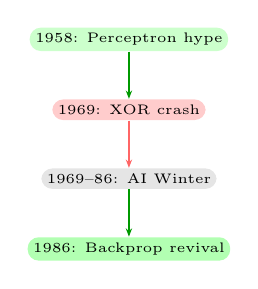
\begin{tikzpicture}[font=\tiny, node distance=0.6cm]
        \node[fill=green!20, rounded corners, inner sep=2pt]
          (hype) {1958: Perceptron hype};
        \node[fill=red!20, rounded corners, inner sep=2pt, below=of hype]
          (crash) {1969: XOR crash};
        \node[fill=gray!20, rounded corners, inner sep=2pt, below=of crash]
          (winter) {1969--86: AI Winter};
        \node[fill=green!30, rounded corners, inner sep=2pt, below=of winter]
          (back) {1986: Backprop revival};
        \draw[-{Stealth[length=3pt]}, thick, green!60!black]
          (hype) -- (crash);
        \draw[-{Stealth[length=3pt]}, thick, red!60]
          (crash) -- (winter);
        \draw[-{Stealth[length=3pt]}, thick, green!60!black]
          (winter) -- (back);
      \end{tikzpicture}
    \end{column}
  \end{columns}

  \note{
    ``When backpropagation showed that multi-layer networks could learn,
    neural networks came roaring back.''

    The Rumelhart/Hinton/Williams 1986 paper was already covered in Slide~22
    (Section~2, Calculus). Cross-reference explicitly: ``Remember the chain
    rule? This is where it saved an entire field.''
  }
\end{frame}

% ----------------------------------------------------------
% Slide 59: Activation Functions
% ----------------------------------------------------------
\begin{frame}{Activation Functions --- The Spice That Makes It Work}

  \begin{columns}[T]
    \begin{column}{0.55\textwidth}
      \begin{insightbox}
        Without a nonlinear activation function, a multi-layer network
        collapses to a single layer. Activation functions give neural
        networks their power.
      \end{insightbox}

      \vspace{0.2em}
      {\small
      \textbf{Sigmoid} --- $\displaystyle\frac{1}{1+e^{-x}}$\par
      \begin{itemize}\setlength\itemsep{1pt}
        \item Smooth S-curve, used 1980s--2000s
        \item Related to the logistic function of
              \textbf{Pierre Fran\c{c}ois Verhulst} (1804--1849,
              Brussels), who modelled population growth (1838)
      \end{itemize}

      \textbf{ReLU} --- $\max(0, x)$\par
      \begin{itemize}\setlength\itemsep{1pt}
        \item Popularised by \textbf{Nair \& Hinton} (2010)
        \item Simpler, faster, avoids vanishing gradients
      \end{itemize}

      \textbf{GELU} --- used in GPT and BERT\par
      \begin{itemize}\setlength\itemsep{1pt}
        \item Introduced by \textbf{Hendrycks \& Gimpel} (2016)
        \item Smooth version of ReLU; used in modern transformers
      \end{itemize}
      }
    \end{column}

    \begin{column}{0.42\textwidth}
      \visualplaceholder[5cm]{Three activation function curves plotted
      side by side: Sigmoid (smooth S-curve, labelled ``1980s--2000s''),
      ReLU (hockey stick, labelled ``2010s''), GELU (smooth ReLU,
      labelled ``2016--present, used in GPT'').
      Caption: ``These simple curves make neural networks nonlinear
      --- and therefore powerful.''}
    \end{column}
  \end{columns}

  \note{
    ``Without activation functions, stacking 100 layers of matrix
    multiplication would be the same as one layer. The activation function
    adds the nonlinearity. It is a small thing that makes everything
    else work.''

    \verifytag{Verhulst logistic function dates --- 1838 or 1845 or both?}
    \verifytag{Nair/Hinton 2010 ICML paper as key popularisation; ReLU-like
    functions appeared earlier (Hahnloser et al.\ 2000).}
    \verifytag{Hendrycks/Gimpel 2016 GELU paper.}
  }
\end{frame}

% ----------------------------------------------------------
% Slide 60: Residual Connections (ResNet)
% ----------------------------------------------------------
\begin{frame}{Residual Connections --- The Trick That Enabled Depth}

  \begin{columns}[T]
    \begin{column}{0.52\textwidth}
      \begin{personbox}[{Kaiming He et al.\ (b.\,c.\,1984)}]{aiViolet}
        \textbf{Origin:} China / USA\\[3pt]
        \textbf{Key paper (2015):} \emph{``Deep Residual Learning for
        Image Recognition''} (ResNet).\\[3pt]
        Instead of each layer computing a completely new output,
        it computes a \alert{change} to the input:
        \[ \text{output} = \text{input} + \text{layer}(\text{input}) \]
        This simple idea allowed networks to grow from
        $\sim$20~layers to 152~layers --- and beyond.
      \end{personbox}

      \vspace{0.3em}
      \begin{insightbox}
        The ``\textbf{Add}'' in the transformer's ``Add \& Norm'' block
        IS He's residual connection from 2015.
        Without it, transformers could not be deep.
      \end{insightbox}
    \end{column}

    \begin{column}{0.45\textwidth}
      \visualplaceholder[5.5cm]{Side-by-side comparison: Left --- standard
      deep network with signal fading layer by layer (fading colour).
      Right --- ResNet with skip connections; an arrow skips over each block,
      carrying the original signal forward.
      Below: residual formula as diagram: input $\to$ [layer] $\to$
      ADD input back $\to$ output.}
    \end{column}
  \end{columns}

  \note{
    ``He's insight was deceptively simple: instead of asking each layer to
    compute the full answer, ask it to compute the DIFFERENCE from the
    input. If a layer has nothing useful to add, it can output zero and
    the input passes through unchanged.''

    LLM connection: ``Every transformer block has a residual connection.''
  }
\end{frame}

% ----------------------------------------------------------
% Slide 61: Layer Normalization and Dropout
% ----------------------------------------------------------
\begin{frame}{Layer Normalization \& Dropout --- Stabilising Deep Networks}

  \begin{columns}[T]
    \begin{column}{0.52\textwidth}
      \begin{personbox}[Ba/Kiros/Hinton -- Layer Norm (2016)]{aiViolet}
        Adjusts the outputs of each layer so they have a consistent
        mean and variance. Stabilises training and speeds convergence.
      \end{personbox}

      \vspace{0.3em}

      \begin{personbox}[Srivastava/Hinton et al. -- Dropout (2014)]{aiViolet}
        Randomly deactivates neurons during training, forcing the network
        to learn robust features rather than memorising.\\[3pt]
        \emph{Like studying for an exam by covering random notes --- you
        learn the material, not the page layout.}
      \end{personbox}

      \vspace{0.3em}
      {\small\textbf{Layer Norm recipe:}
        (1)~Compute the average of all neuron outputs in a layer.
        (2)~Compute how spread out they are.
        (3)~Subtract the average and divide by the spread.
        Now they are centred at zero with consistent scale.}
    \end{column}

    \begin{column}{0.45\textwidth}
      \visualplaceholder[5.5cm]{Top: Layer normalisation --- a row of neuron
      activations before (wildly varying) and after normalisation (centred,
      consistent). Caption: ``Layer Norm = rescale so nothing explodes.''
      Bottom: Dropout --- a network with some neurons crossed out.
      Caption: ``Dropout = randomly disable neurons during training.''}

      \vspace{0.3em}
      \begin{tcolorbox}[colback=aiViolet!5,colframe=aiViolet!60,
        boxrule=0.5pt,rounded corners,left=3pt,right=3pt,top=2pt,bottom=2pt]
        \small In the transformer's ``Add \& Norm'':\\
        \textbf{Add} = He's residual connection (Slide~60)\\
        \textbf{Norm} = Ba's layer normalisation
      \end{tcolorbox}
    \end{column}
  \end{columns}

  \note{
    ``Layer normalisation is the `Norm' in the transformer's `Add \& Norm.'
    Dropout is used during training. Both are invisible to the user but
    essential for making deep networks work.''

    \verifytag{Ba et al.\ 2016 --- arXiv preprint, not initially peer-reviewed.}
    \verifytag{Srivastava et al.\ 2014 JMLR as definitive paper; Hinton
    proposed the idea earlier in 2012.}
  }
\end{frame}

% ----------------------------------------------------------
% Slide 62: Convergence Diagram Update -- The Neuron & Depth
% ----------------------------------------------------------
\begin{frame}{Convergence Diagram --- The Neuron \& Depth Lights Up}

  \visualplaceholder[10cm]{Convergence diagram: ``The Neuron \& Depth'' node
  now lit in yellow/gold. 7 of 10 nodes active.
  Label: ``Activation + normalisation + residuals = deep networks.''}

  \vspace{0.3em}
  \begin{columns}[T]
    \begin{column}{0.48\textwidth}
      \begin{tcolorbox}[colback=aiViolet!5,colframe=aiViolet,
        fonttitle=\bfseries\small,title={Section 7 Summary},
        rounded corners,boxrule=0.8pt,left=3pt,right=3pt,top=3pt,bottom=3pt]
        \scriptsize
        \begin{tabular}{@{}ll@{}}
          McCulloch-Pitts (1943)    & First math neuron\\
          Rosenblatt (1958)         & Perceptron learns\\
          Minsky/Papert (1969)      & XOR, AI winter\\
          Rumelhart/Hinton/W.\ (1986) & Multi-layer revival\\
          Verhulst (1838) $\to$ Sigmoid & Population $\to$ activation\\
          Nair/Hinton (2010)        & ReLU\\
          Srivastava et al.\ (2014)  & Dropout\\
          He et al.\ (2015)         & Residual connections\\
          Ba et al.\ (2016)         & Layer normalisation\\
          Hendrycks/Gimpel (2016)   & GELU
        \end{tabular}
      \end{tcolorbox}
    \end{column}

    \begin{column}{0.48\textwidth}
      \begin{tcolorbox}[colback=accentOrange!8,colframe=accentOrange,
        fonttitle=\bfseries\small,
        title={\faArrowRight\ Connection to the Transformer},
        rounded corners,boxrule=0.8pt,left=3pt,right=3pt,top=3pt,bottom=3pt]
        \scriptsize
        The artificial neuron, with its activation function, is the basic
        unit. Residual connections, layer normalisation, and dropout allow
        transformers to be DEEP. There are billions of neurons in GPT,
        stacked 96+ layers.
      \end{tcolorbox}
    \end{column}
  \end{columns}

  \note{
    Transition: ``We can build neurons, stack them into deep layers, and
    train them. But language is SEQUENTIAL --- word order matters.
    How do you process a sequence? That took another set of inventions.''
  }
\end{frame}


% ============================================================
% SECTION 8: SEQUENCE MODELING (Slides 63--68)
% "The Path to Language"
% Timeline: 1906--2014
% ============================================================
\section{Sequence Modeling}

% ----------------------------------------------------------
% Slide 63: Section Divider
% ----------------------------------------------------------
{
\setbeamercolor{background canvas}{bg=aiViolet}
\begin{frame}[plain]
  \centering
  \vspace{1.8cm}
  \textcolor{white}{\Huge\bfseries Sequence Modeling}\\[0.5em]
  \textcolor{white}{\Large The Path to Language}\\[1em]
  \textcolor{white!80}{\large 1906--2014}\\[1.5em]
  \textcolor{white!60}{\normalsize Markov \(\cdot\) Baum \(\cdot\) Elman
    \(\cdot\) Hochreiter \& Schmidhuber \(\cdot\) Bahdanau}\\[1em]
  \textcolor{white!50}{\small Language is a sequence.
  Modeling sequences required 100 years of invention.}

  \note{
    Convergence diagram: Section 8 node pulsing.

    ``Language is sequential --- word order matters. `Dog bites man' is
    very different from `Man bites dog.' How do you process a sequence?''
  }
\end{frame}
}

% ----------------------------------------------------------
% Slide 64: Markov Chains
% ----------------------------------------------------------
\begin{frame}{Andrey Markov --- The Simplest Language Model}

  \begin{columns}[T]
    \begin{column}{0.52\textwidth}
      \begin{personbox}[Andrey Andreyevich Markov (1856--1922)]{aiViolet}
        \textbf{Origin:} Ryazan, Russia\\[3pt]
        Introduced \textbf{Markov chains} (1906) by analysing the
        alternation of vowels and consonants in Pushkin's poem
        \emph{Eugene Onegin}.\\[3pt]
        He was \emph{not} studying language --- he was disproving a
        claim that the law of large numbers required independence.
        But his method became the foundation of all sequence modelling.
      \end{personbox}

      \vspace{0.3em}
      \begin{insightbox}
        A Markov chain predicts the next state based \emph{only} on the
        current state, ignoring all history. Your phone's autocomplete
        is a descendant of this idea.
      \end{insightbox}
    \end{column}

    \begin{column}{0.45\textwidth}
      \visualplaceholder[5.5cm]{Top: State diagram --- states are words
      (``the'', ``cat'', ``sat'', ``on''), arrows labelled with
      transition probabilities.
      Bottom: Text generated by a Markov chain vs.\ text from an LLM.
      Markov text is grammatical locally but incoherent globally.}
    \end{column}
  \end{columns}

  \note{
    ``Markov analysed poetry to prove a point about probability theory.
    His chain model became the ancestor of every language model, including
    the one in your phone's autocomplete.''

    \verifytag{``Eugene Onegin'' analysis dated to 1913 in some sources,
    while the mathematical framework was published 1906. Clarify the
    distinction.}
  }
\end{frame}

% ----------------------------------------------------------
% Slide 65: Hidden Markov Models
% ----------------------------------------------------------
\begin{frame}{Hidden Markov Models --- Adding Depth}

  \begin{columns}[T]
    \begin{column}{0.52\textwidth}
      \begin{personbox}[Leonard Baum et al.\ (1960s--1972)]{aiViolet}
        \textbf{Origin:} USA\\[3pt]
        Developed the mathematical framework for \textbf{Hidden Markov
        Models} (HMMs) and the \textbf{Baum--Welch algorithm} for
        training them.\\[3pt]
        HMMs add a hidden state layer: the observed output depends on
        an unobserved internal state that must be inferred.
      \end{personbox}

      \vspace{0.3em}
      \begin{insightbox}
        Speech recognition used HMMs for 30+ years before deep learning
        replaced them. The idea of ``hidden internal states'' producing
        observable outputs is conceptually similar to the hidden layers
        of a neural network.
      \end{insightbox}
    \end{column}

    \begin{column}{0.45\textwidth}
      \visualplaceholder[5.5cm]{HMM diagram: hidden states on top (connected
      by transition arrows), observed outputs below (connected to hidden
      states by emission arrows).
      Caption: ``The hidden states cannot be seen directly --- they must
      be inferred from observations.''}
    \end{column}
  \end{columns}

  \note{
    ``HMMs dominated speech recognition from the 1970s through the 2010s.
    Siri's original speech engine used HMMs.''

    \verifytag{Baum--Welch algorithm dates: key papers 1966, 1970, 1972.
    Baum's full name and dates are surprisingly hard to pin down.}
  }
\end{frame}

% ----------------------------------------------------------
% Slide 66: Recurrent Neural Networks
% ----------------------------------------------------------
\begin{frame}{Recurrent Neural Networks --- Memory in a Loop}

  \begin{columns}[T]
    \begin{column}{0.52\textwidth}
      \begin{personbox}[Michael Jordan -- Jordan Network (1986)]{aiViolet}
        \textbf{Origin:} USA\\[3pt]
        An early form of recurrent neural network.\\
        \emph{Yes, the field has its own Michael Jordan.}
      \end{personbox}

      \vspace{0.2em}

      \begin{personbox}[Jeffrey Elman (1948--2018) --- Elman Network (1990)]{aiViolet}
        \textbf{Origin:} USA\\[3pt]
        The hidden state at time $t$ is fed back as input at time $t{+}1$.
        This is the standard form of RNN.
      \end{personbox}

      \vspace{0.2em}
      \begin{tcolorbox}[colback=red!5,colframe=red!60,
        boxrule=0.5pt,rounded corners,left=3pt,right=3pt,top=2pt,bottom=2pt]
        \small\textbf{Fatal flaw:} The hidden state gets overwritten
        at each step. After 50~words, the memory of word~1 has been
        washed away. This is the \alert{vanishing gradient problem}.
      \end{tcolorbox}
    \end{column}

    \begin{column}{0.45\textwidth}
      \visualplaceholder[5.5cm]{An RNN unrolled across time steps: the same
      network processing word 1, then word 2, then word 3, with the
      hidden state carried forward like a ``memory'' arrow.
      Caption: ``The hidden state is the RNN's memory. But it is a
      very leaky memory.''}
    \end{column}
  \end{columns}

  \note{
    ``RNNs have a fatal flaw: the hidden state gets overwritten at each step.
    By the time you have read 50 words, the memory of word 1 has been
    washed away. This is the vanishing gradient problem.''

    \verifytag{Jordan 1986 --- sometimes cited as 1986 technical report.}
  }
\end{frame}

% ----------------------------------------------------------
% Slide 67: LSTM [EXTENDED]
% ----------------------------------------------------------
\begin{frame}{LSTM --- Long Short-Term Memory
  \hfill\small\textcolor{gray}{[EXTENDED]}}

  \begin{columns}[T]
    \begin{column}{0.52\textwidth}
      \begin{personbox}[Hochreiter \& Schmidhuber]{aiViolet}
        \textbf{Sepp Hochreiter:} Austria\\
        \textbf{J\"urgen Schmidhuber:} Munich, Germany\\[3pt]
        Published \emph{``Long Short-Term Memory''} (1997).\\[3pt]
        Hochreiter's diploma thesis (1991, supervised by Schmidhuber)
        identified the vanishing gradient problem. The 1997 LSTM paper
        provided the solution: explicit \textbf{memory cells} with
        \textbf{gates} that control what to remember and what to forget.
      \end{personbox}

      \vspace{0.3em}
      \begin{insightbox}
        LSTM dominated language tasks from the late 1990s through 2017.
        Google Translate used LSTMs. But LSTMs process words
        \emph{one at a time} --- you cannot parallelise them.
        This bottleneck led to \alert{attention}.
      \end{insightbox}
    \end{column}

    \begin{column}{0.45\textwidth}
      \visualplaceholder[5.5cm]{Simplified LSTM cell: input gate, forget
      gate, output gate, cell state. Caption: ``The forget gate decides
      what to remember. The input gate decides what is new. The output
      gate decides what to reveal.''}
    \end{column}
  \end{columns}

  \note{
    ``LSTM solved the memory problem. But it introduced a new bottleneck:
    sequential processing. You cannot parallelise an LSTM --- each word
    must wait for the previous one. For long documents, this is painfully
    slow. The key idea that changed everything: attention.''

    This slide is EXTENDED --- can cut if short on time. Mention LSTM
    en route to attention if skipping.

    \verifytag{Hochreiter 1991 diploma thesis as vanishing gradient analysis.}
  }
\end{frame}

% ----------------------------------------------------------
% Slide 68: The Attention Mechanism -- KEY BREAKTHROUGH
% ----------------------------------------------------------
\begin{frame}{The Attention Mechanism --- The Bridge to Transformers}

  \begin{columns}[T]
    \begin{column}{0.52\textwidth}
      \begin{personbox}[Bahdanau/Cho/Bengio (2014)]{aiViolet}
        \textbf{Dzmitry Bahdanau:} Belarus/Canada\\
        \textbf{Kyunghyun Cho:} South Korea/Canada\\
        \textbf{Yoshua Bengio:} France/Canada\\[3pt]
        Published \emph{``Neural Machine Translation by Jointly Learning
        to Align and Translate''} (2014 arXiv; 2015 ICLR).\\[3pt]
        \textbf{Key insight:} Instead of compressing the entire input
        into a fixed-size vector, let the model \alert{look back}
        at all previous positions and decide which ones are relevant.
      \end{personbox}

      \vspace{0.3em}
      \begin{tcolorbox}[colback=aiViolet!8,colframe=aiViolet,
        fonttitle=\bfseries,title={The Breakthrough},
        rounded corners,boxrule=1pt,left=4pt,right=4pt,top=3pt,bottom=3pt]
        \small \textbf{Attention} = the ability to look back and focus.\\[3pt]
        Without this 2014 paper, there would be no GPT,
        no Claude, no ChatGPT.
      \end{tcolorbox}
    \end{column}

    \begin{column}{0.45\textwidth}
      \visualplaceholder[5.5cm]{Top: Attention diagram --- translating
      ``Le chat est sur le tapis.'' When generating ``cat,'' the model
      attends strongly to ``chat.'' When generating ``mat,'' it attends
      to ``tapis.'' Colour-coded attention weights shown as lines of
      varying thickness.
      Bottom: Comparison --- RNN (compresses everything into one vector)
      vs.\ Attention (can look back at everything).}
    \end{column}
  \end{columns}

  \note{
    ``Bahdanau's insight was simple but transformative: why compress
    everything into one vector when you can look back at the whole input?
    This idea --- attention --- became the core of the transformer.''

    Give this slide weight. It is the key intellectual bridge.

    Convergence diagram update: ``Sequence Modeling'' node lit in teal.
    Label: ``Attention = context.''

    Transition: ``We now have ALL the building blocks. It is time to
    put them together.''
  }
\end{frame}


% ============================================================
% SECTION 9: THE TRANSFORMER (Slides 69--74)
% "Where Everything Converges"
% Timeline: 2017
% ============================================================
\section{The Transformer}

% ----------------------------------------------------------
% Slide 69: Section Divider
% ----------------------------------------------------------
{
\setbeamercolor{background canvas}{bg=aiViolet}
\begin{frame}[plain]
  \centering
  \vspace{1.6cm}
  \textcolor{white}{\Huge\bfseries The Transformer}\\[0.5em]
  \textcolor{white}{\Large Where Everything Converges}\\[1em]
  \textcolor{white!80}{\large 2017}\\[1.5em]
  \textcolor{white!60}{\normalsize Vaswani \(\cdot\) Shazeer \(\cdot\)
    Parmar \(\cdot\) Uszkoreit \(\cdot\) Jones}\\[0.2em]
  \textcolor{white!60}{\normalsize Gomez \(\cdot\) Kaiser \(\cdot\)
    Polosukhin}\\[1em]
  \textcolor{white!50}{\small Eight branches of mathematics meet
  in one architecture.}\\[0.3em]
  \textcolor{white!40}{\footnotesize\itshape ``Attention Is All You Need.''}

  \note{
    Convergence diagram: 8 of 10 nodes lit. Section 9 pulsing.

    ``2017: Eight branches of mathematics, developed over more than two
    millennia, all converge in one architecture.''
  }
\end{frame}
}

% ----------------------------------------------------------
% Slide 70: "Attention Is All You Need"
% ----------------------------------------------------------
\begin{frame}{``Attention Is All You Need'' --- The Paper That Changed AI}

  \begin{columns}[T]
    \begin{column}{0.55\textwidth}
      {\small In 2017, a team at Google published a paper proposing an
      architecture that used \textbf{only attention} --- no recurrence,
      no convolution. It was simpler, faster, and better.}

      \vspace{0.4em}

      \begin{personbox}[The Eight Authors (2017 NeurIPS)]{aiViolet}
        \textbf{Ashish Vaswani}, \textbf{Noam Shazeer},
        \textbf{Niki Parmar}, \textbf{Jakob Uszkoreit},
        \textbf{Llion Jones}, \textbf{Aidan Gomez},
        \textbf{{\L}ukasz Kaiser}, \textbf{Illia Polosukhin}\\[3pt]
        Most in their 20s and 30s. Several have since founded major AI
        companies (Cohere, Character.AI).
      \end{personbox}

      \vspace{0.3em}
      \begin{insightbox}
        Eight researchers. One paper. The architecture that powers
        \emph{every} major LLM.
      \end{insightbox}
    \end{column}

    \begin{column}{0.42\textwidth}
      \visualplaceholder[5cm]{Top: The first page of ``Attention Is All You
      Need'' with title highlighted.
      Bottom: Stylised portraits or photos of the eight authors.
      Caption: ``Eight researchers. One paper. One architecture.''}
    \end{column}
  \end{columns}

  \note{
    ``The title is bold: `Attention Is All You Need.' They were right.
    This single architecture --- the transformer --- is the foundation of
    GPT, Claude, Gemini, and virtually every LLM in existence.''

    \verifytag{Gomez founded Cohere; Jones and Shazeer co-founded
    Character.AI. Confirm details.}
  }
\end{frame}

% ----------------------------------------------------------
% Slide 71: Self-Attention -- The Core Mechanism
% ----------------------------------------------------------
\begin{frame}{Self-Attention --- The Core Mechanism}

  {\small Each token generates three vectors: a \textbf{Query}
  (``what am I looking for?''), a \textbf{Key} (``what do I contain?''),
  and a \textbf{Value} (``what information do I carry?'').}

  \vspace{0.3em}

  % Step-by-step with back-references
  \begin{tcolorbox}[colback=aiViolet!5,colframe=aiViolet,
    fonttitle=\bfseries,title={Self-Attention Step by Step},
    rounded corners,boxrule=0.8pt,left=4pt,right=4pt,top=4pt,bottom=4pt]
    \small
    \begin{enumerate}\setlength\itemsep{2pt}
      \item Compute attention scores: \textbf{dot product} of each Query
            with each Key \hfill\textcolor{gray}{\scriptsize(Gibbs, Slide~10)}
      \item Scale scores: divide by $\sqrt{d}$ to keep numbers
            manageable \hfill\textcolor{gray}{\scriptsize(cosine-like scaling, Slide~11)}
      \item Normalise with \textbf{softmax}: scores become
            probabilities \hfill\textcolor{gray}{\scriptsize(Boltzmann, Slide~33)}
      \item Output = weighted sum of Values via
            \textbf{matrix multiplication}
            \hfill\textcolor{gray}{\scriptsize(Cayley, Slide~9)}
    \end{enumerate}
  \end{tcolorbox}

  \vspace{0.2em}

  % Formal inset
  \begin{columns}[T]
    \begin{column}{0.48\textwidth}
      \begin{tcolorbox}[colback=gray!5,colframe=gray!40,
        boxrule=0.5pt,rounded corners,left=3pt,right=3pt,top=2pt,bottom=2pt]
        {\scriptsize\textbf{Formal notation (small inset):}
        \[
          \text{Attention}(Q,K,V)
            = \text{softmax}\!\left(\frac{Q K^{\!\top}}{\sqrt{d_k}}\right) V
        \]
        $K^{\!\top}$ means ``flip the matrix on its side'' (transpose).}
      \end{tcolorbox}
    \end{column}
    \begin{column}{0.48\textwidth}
      {\small\textbf{Concrete example:} In ``The cat sat on the mat because
      \emph{it} was tired,'' the word ``it'' attends most strongly to
      ``cat.'' Self-attention learns that ``it'' refers to ``cat.''}
    \end{column}
  \end{columns}

  \note{
    ``Self-attention is the convergence point. Linear algebra, probability,
    and information theory, all in one equation.''

    Walk through the concrete ``it'' $\to$ ``cat'' example. This is how
    the model resolves references across a sentence.
  }
\end{frame}

% ----------------------------------------------------------
% Slide 72: Feed-Forward Block and Multi-Head Attention
% ----------------------------------------------------------
\begin{frame}{Multi-Head Attention \& Feed-Forward Networks}

  \begin{columns}[T]
    \begin{column}{0.52\textwidth}
      \textbf{Multi-Head Attention}\\[3pt]
      {\small Instead of one set of Q/K/V, the transformer uses multiple
      ``heads'' (8, 12, or more) in parallel. Each head learns different
      relationships: syntax, semantics, position, etc.
      Results are concatenated and projected back.}

      \vspace{0.5em}
      \textbf{Feed-Forward Network (FFN)}\\[3pt]
      {\small Two matrix multiplications with a GELU activation in between.
      This is the universal approximation theorem
      (Cybenko, Slide~52) applied within each transformer layer ---
      the FFN provides the raw computational power.}

      \vspace{0.5em}
      \begin{insightbox}
        \small One transformer layer = Attention + FFN + two rounds of
        ``Add \& Norm.'' Stack 96 of these and you have GPT-4.
      \end{insightbox}
    \end{column}

    \begin{column}{0.45\textwidth}
      \visualplaceholder[5.5cm]{A single transformer block, annotated:
      Multi-Head Attention sub-block $\to$ Add \& Norm
      (residual + layer norm, Slides 60--61) $\to$
      Feed-Forward Network sub-block $\to$ Add \& Norm.
      Every component labelled with its origin section.}
    \end{column}
  \end{columns}

  \note{
    ``One transformer layer = attention + feed-forward + two rounds of
    `add and normalise.' Stack 96 of these layers and you have GPT-4.
    Every component was taught in an earlier section of this lecture.''
  }
\end{frame}

% ----------------------------------------------------------
% Slide 73: THE CLIMAX -- Full Annotated Transformer Diagram
% ----------------------------------------------------------
\begin{frame}{The Full Transformer --- Annotated with 2,000+ Years of Math}

  % Large placeholder -- THIS IS THE LECTURE'S CLIMAX
  \visualplaceholder[13cm]{%
    \textbf{CLIMAX DIAGRAM --- Full decoder-only transformer architecture}\\[4pt]
    Annotated components (back-references to earlier slides):\\
    \textbullet\ \textbf{Input Embedding:} Words $\to$ Vectors
      (Grassmann 1844, Mikolov 2013, Slide~14)\\
    \textbullet\ \textbf{Positional Encoding:} Sine/cosine
      (Fourier 1807, Slide~50)\\
    \textbullet\ \textbf{Multi-Head Self-Attention:} Dot product + softmax
      + matrix mult.\ (Gibbs 1880s Slide~10, Boltzmann 1870s Slide~33,
      Cayley 1858 Slide~9, Bahdanau 2014 Slide~68)\\
    \textbullet\ \textbf{Add \& Norm:} Residual + Layer Norm
      (He 2015 Slide~60, Ba 2016 Slide~61)\\
    \textbullet\ \textbf{FFN:} Matrix mult.\ + GELU
      (Cybenko 1989 Slide~52, Hendrycks 2016 Slide~59)\\
    \textbullet\ \textbf{Dropout:} (Srivastava/Hinton 2014 Slide~61)\\
    \textbullet\ \textbf{Output Softmax:} Probability over vocabulary
      (Fisher 1922, Boltzmann/Luce Slide~33)\\
    \textbullet\ \textbf{Training:} Cross-entropy + backprop + SGD
      (Shannon 1948, Cauchy 1847, Linnainmaa 1970)\\
    \textbullet\ \textbf{Hardware:} GPU arrays
      (NVIDIA CUDA 2007, AlexNet 2012 Slide~47)%
  }

  \vspace{0.3em}
  \begin{tcolorbox}[colback=accentOrange!10,colframe=accentOrange,
    fonttitle=\bfseries,
    title={\faUsers\ Interactive Moment: ``Count the Building Blocks''},
    rounded corners,boxrule=1pt,left=4pt,right=4pt,top=3pt,bottom=3pt]
    \small Students: look at this diagram and try to identify which of
    the 10~sections each component comes from. How many can you find?
    \hfill\emph{(3~min)}
  \end{tcolorbox}

  \note{
    THIS IS THE CENTRAL THESIS OF THE ENTIRE LECTURE, crystallised in
    one diagram. Let this land. \textbf{Pause.}

    ``Look at this diagram. Every single piece has a history. The sine
    functions come from Fourier in 1807. The matrix multiplications come
    from Cayley in 1858. The softmax comes from Boltzmann in the 1870s.
    The training algorithm uses Cauchy's gradient descent from 1847 and
    Linnainmaa's automatic differentiation from 1970. The residual
    connections come from He in 2015. The layer normalisation from Ba in
    2016. When you talk to an AI, you are talking to 2,000 years of
    mathematics, all running at once.''

    Interactive moment: give students 3 minutes to ``count the building
    blocks'' --- identify which of the 10 sections each component comes
    from.
  }
\end{frame}

% ----------------------------------------------------------
% Slide 74: Positional Encoding -- Fourier Meets Transformers
% ----------------------------------------------------------
\begin{frame}{Positional Encoding --- Fourier Meets Transformers}

  \begin{columns}[T]
    \begin{column}{0.52\textwidth}
      {\small Transformers have no built-in notion of word order (unlike
      RNNs). To fix this, they add \textbf{positional encodings} ---
      sine and cosine functions at different frequencies.
      This is Fourier's idea, applied directly.}

      \vspace{0.4em}

      \textbf{Recipe (CONCEPTUAL):}\\
      {\small For each position in the sentence and each dimension in
      the vector, compute a sine or cosine wave with a specific
      frequency. Different dimensions use different frequencies ---
      just like Fourier's decomposition. Each position gets a unique
      ``fingerprint'' of wave values.}

      \vspace{0.3em}

      % Formal inset
      \begin{tcolorbox}[colback=gray!5,colframe=gray!40,
        boxrule=0.5pt,rounded corners,left=3pt,right=3pt,top=2pt,bottom=2pt]
        {\scriptsize\textbf{Formal:}
        \begin{align*}
          PE(\text{pos}, 2i) &= \sin\!\bigl(\text{pos}\, /\, 10000^{2i/d}\bigr)\\
          PE(\text{pos}, 2i{+}1) &= \cos\!\bigl(\text{pos}\, /\, 10000^{2i/d}\bigr)
        \end{align*}
        The $10000^{2i/d}$ creates a spectrum of frequencies from
        very slow to very fast.}
      \end{tcolorbox}
    \end{column}

    \begin{column}{0.45\textwidth}
      \visualplaceholder[5.5cm]{Heatmap of positional encodings:
      rows = positions (1st word, 2nd word, \ldots, 100th word),
      columns = dimensions. Clear sinusoidal wave patterns visible.
      Caption: ``Fourier's sine and cosine waves, used to tell
      the transformer which word is which.''}

      \vspace{0.3em}
      \begin{insightbox}
        Fourier decomposed heat into waves.
        Vaswani decomposed word position into waves.
        Same math, 210 years apart.
      \end{insightbox}
    \end{column}
  \end{columns}

  \note{
    ``Fourier decomposed heat into waves. Vaswani decomposed word
    position into waves. The same math, 210 years apart, for completely
    different purposes.''

    Convergence diagram update: ALL 10 nodes now lit (Sections 9 and 10).
    Central ``?'' becomes ``TRANSFORMER.'' The full convergence diagram
    is complete.
  }
\end{frame}


% ============================================================
% SECTION 10: SCALING TO LLMs + CLOSING (Slides 75--78)
% "The Final Leap"
% Timeline: 2018--2026
% ============================================================
\section{Scaling to LLMs}

% ----------------------------------------------------------
% Slide 75: The Scaling Leap
% ----------------------------------------------------------
\begin{frame}{The Scaling Leap --- From Transformer to LLM}

  \begin{columns}[T]
    \begin{column}{0.52\textwidth}
      {\small The transformer architecture, scaled up with more parameters,
      more data, and more compute, produces Large Language Models with
      emergent abilities.}

      \vspace{0.3em}

      \begin{tcolorbox}[colback=aiViolet!5,colframe=aiViolet,
        fonttitle=\bfseries\small,title={The GPT Series},
        rounded corners,boxrule=0.8pt,left=3pt,right=3pt,top=3pt,bottom=3pt]
        \scriptsize
        \begin{tabular}{@{}lrl@{}}
          \textbf{GPT-1} (2018) & 117M params & Pre-train + fine-tune\\
          \textbf{GPT-2} (2019) & 1.5B params & Convincing text gen.\\
          \textbf{GPT-3} (2020) & 175B params & Few-shot learning\\
          \textbf{GPT-4} (2023) & undisclosed & Multimodal\\
          \textbf{Claude} (2023--26) & --- & Constitutional AI
        \end{tabular}
      \end{tcolorbox}

      \vspace{0.3em}

      \begin{personbox}[Jared Kaplan et al.\ (2020) --- Scaling Laws]{aiViolet}
        \scriptsize LLM performance scales as a smooth \textbf{power law}
        with compute, data, and parameters. Predictable improvement.
      \end{personbox}
    \end{column}

    \begin{column}{0.45\textwidth}
      \visualplaceholder[5.5cm]{Top: Log-log plot of parameter count vs.\
      year: GPT-1 (2018) $\to$ GPT-2 (2019) $\to$ GPT-3 (2020) $\to$
      PaLM (2022) $\to$ GPT-4 (2023) $\to$ frontier models (2025--26).
      Exponential growth visible.
      Bottom: Timeline of key milestones: RLHF (2017), InstructGPT (2022),
      ChatGPT (Nov 2022), GPT-4 (Mar 2023), Claude~3 (2024), open-source
      explosion (Llama, Mistral).}
    \end{column}
  \end{columns}

  \note{
    ``The transformer is the same architecture from 2017. What changed is
    scale. More parameters, more training data, more compute. And somewhere
    along the way, these models started doing things nobody programmed them
    to do --- reasoning, writing code, translating languages they were
    barely trained on.''

    \verifytag{Kaplan et al.\ 2020 scaling laws paper.}
    \verifytag{ChatGPT launch: November 30, 2022.}
    \verifytag{Christiano et al.\ 2017 for RLHF.}
  }
\end{frame}

% ----------------------------------------------------------
% Slide 76: Return to the Exploded Diagram
% ----------------------------------------------------------
\begin{frame}{Return to the Exploded Diagram --- Now You Understand Every Piece}

  \visualplaceholder[13cm]{%
    \textbf{The SAME exploded transformer diagram from Slide~3},
    now with every label including the mathematician's name, date,
    AND slide number:\\[3pt]
    \textbullet\ Matrix multiplication (Cayley, 1858 --- Slide~9)
    \textbullet\ Dot product (Gibbs, 1880s --- Slide~10)\\
    \textbullet\ Gradient descent (Cauchy, 1847 --- Slide~21)
    \textbullet\ Softmax (Boltzmann, 1870s --- Slide~33)\\
    \textbullet\ Cross-entropy (Shannon, 1948 --- Slide~37)
    \textbullet\ Backpropagation (Linnainmaa 1970, Rumelhart/Hinton/Williams
    1986 --- Slide~22)\\
    \textbullet\ Activation functions (Verhulst 1838, Nair/Hinton 2010
    --- Slide~59)\\
    \textbullet\ Residual connections (He et al.\ 2015 --- Slide~60)
    \textbullet\ Layer norm (Ba et al.\ 2016 --- Slide~61)\\
    \textbullet\ Self-attention (Bahdanau 2014, Vaswani 2017
    --- Slides~68, 71)\\
    \textbullet\ Positional encoding (Fourier 1807 --- Slide~74)
    \textbullet\ GPU computing (NVIDIA CUDA 2007 --- Slide~47)%
  }

  \note{
    ``At the start of this lecture, this diagram was overwhelming.
    Now you can point to each piece and say who invented it, when,
    and why. That is the power of understanding the history.''

    Caption on slide: ``You now know the history of every piece of
    this machine.''
  }
\end{frame}

% ----------------------------------------------------------
% Slide 77: Convergence Diagram -- Final State
% ----------------------------------------------------------
\begin{frame}{Convergence Diagram --- Final State}

  \visualplaceholder[10cm]{The completed convergence diagram. All 10 nodes
  lit. Central ``TRANSFORMER'' node glowing. Each node label includes its
  cumulative date range:\\
  1.\ Linear Algebra (1809--2013) --- blue\\
  2.\ Calculus \& Optimisation (c.\,250 BCE--1986) --- green\\
  3.\ Probability \& Statistics (1654--1959) --- orange\\
  4.\ Information Theory (1865--2016) --- red\\
  5.\ Logic \& Computation (1854--2012) --- grey\\
  6.\ Function Approximation (1807--1991) --- purple\\
  7.\ The Neuron \& Depth (1943--2016) --- yellow\\
  8.\ Sequence Modeling (1906--2014) --- teal\\
  9.\ The Transformer (2017) --- multicolour\\
  10.\ Scaling to LLMs (2018--2026) --- gradient}

  \vspace{0.3em}
  \begin{center}
    {\large\bfseries\color{aiViolet}
    Ten streams of human invention, flowing into one machine.}
  \end{center}

  \note{
    Let the diagram speak. This is the visual summary of the entire lecture.
    All 10 nodes active. All arrows visible. 2,000+ years of mathematics
    converging.
  }
\end{frame}

% ----------------------------------------------------------
% Slide 78: Closing -- The Story Is Not Over
% ----------------------------------------------------------
\begin{frame}{The Story Is Not Over}

  \begin{tcolorbox}[colback=aiViolet!8,colframe=aiViolet,
    fonttitle=\bfseries\Large,
    title={\raisebox{-0.2em}{\faInfinity}\ 2,000+ Years of Mathematics.
    One Machine. Your Turn.},
    rounded corners,boxrule=1.5pt,
    left=6pt,right=6pt,top=6pt,bottom=6pt]

    \begin{itemize}\setlength\itemsep{6pt}
      \item Every component of an LLM was invented by someone, for a
            specific purpose, often centuries before AI existed.

      \item Grassmann imagined abstract vector spaces. Boltzmann studied
            gas molecules. Fourier solved the heat equation. Markov
            analysed poetry. Archimedes approximated circles.
            \textbf{None of them imagined AI.}

      \item The math you learn in school --- algebra, calculus,
            probability --- is the \emph{same math} running inside the
            AI you talk to every day.

      \item The next building block has not been invented yet.
            It might come from pure mathematics, from physics, from
            linguistics, from neuroscience ---
            \textbf{or from someone in this room.}
    \end{itemize}
  \end{tcolorbox}

  \vspace{0.3em}
  \visualplaceholder[10cm]{Reprise of the completed convergence diagram
  from Slide~77 / Exploded diagram from Slide~3.
  Below: ``2,000+ years of mathematics. One machine. Your turn.''}

  \note{
    ``When you talk to an AI, you are talking to the accumulated genius
    of Archimedes, Grassmann, Cayley, Newton, Leibniz, Cauchy, Boltzmann,
    Shannon, Turing, Mikolov, McCulloch, Pitts, Rosenblatt, Hochreiter,
    Schmidhuber, Bahdanau, Vaswani, and dozens of others. Two thousand
    years of human curiosity, all running at once, on hardware that
    Boole's algebra made possible. The next invention is yours.''

    Let the final line resonate. End.
  }
\end{frame}


\end{document}
